%%% demothesis.tex ---
%%
%% Filename: demothesis.tex
%% Description:
%% Author: Ola Leifler
%% Maintainer:
%% Created: Thu Oct 14 12:52:20 2010 (CEST)
%% Version: $Id$
%% Version:
%% Last-Updated: Wed Jun 28 10:57:24 2017 (+0200)
%%           By: Ola Leifler
%%     Update #: 169
%% URL:
%% Keywords:
%% Compatibility:
%%
%%%%%%%%%%%%%%%%%%%%%%%%%%%%%%%%%%%%%%%%%%%%%%%%%%%%%%%%%%%%%%%%%%%%%%
%%
%%% Commentary:
%%
%%
%%
%%%%%%%%%%%%%%%%%%%%%%%%%%%%%%%%%%%%%%%%%%%%%%%%%%%%%%%%%%%%%%%%%%%%%%
%%
%%% Change log:
%%
%%
%% RCS $Log$
%%%%%%%%%%%%%%%%%%%%%%%%%%%%%%%%%%%%%%%%%%%%%%%%%%%%%%%%%%%%%%%%%%%%%%
%%
%%% Code:

\documentclass[bachelor,lith,swedish]{liuthesis}
%% Settings go in settings.tex
%%% settings.tex ---
%%
%% Filename: settings.tex
%% Description:
%% Author: Ola Leifler
%% Maintainer:
%% Created: Tue Oct 19 21:11:31 2010 (CEST)
%% Version: $Id$
%% Version:
%% Last-Updated: Tue Apr 25 08:49:48 2017 (+0200)
%%           By: Ola Leifler
%%     Update #: 43
%% URL:
%% Keywords:
%% Compatibility:
%%
%%%%%%%%%%%%%%%%%%%%%%%%%%%%%%%%%%%%%%%%%%%%%%%%%%%%%%%%%%%%%%%%%%%%%%
%%
%%% Commentary:
%%
%%
%%
%%%%%%%%%%%%%%%%%%%%%%%%%%%%%%%%%%%%%%%%%%%%%%%%%%%%%%%%%%%%%%%%%%%%%%
%%
%%% Change log:
%%
%%
%% RCS $Log$
%%%%%%%%%%%%%%%%%%%%%%%%%%%%%%%%%%%%%%%%%%%%%%%%%%%%%%%%%%%%%%%%%%%%%%
%%
%%% Code:

\usepackage[backend=bibtex,sorting=none,style=numeric,natbib=true]{biblatex}
\usepackage{scrextend}
\usepackage{xifthen}
\usepackage{enumitem}
\usepackage{scrextend}
\newcounter{switchcase}

\newcommand{\ifequals}[3]{\ifthenelse{\equal{#1}{#2}}{\stepcounter{switchcase} #3}{}}
\newcommand{\case}[2]{#1 #2} % Dummy, so \renewcommand has something to overwrite...
\newenvironment{switch}[1]{
  %Executed at \begin{switch}
  \setcounter{switchcase}{0}
  \renewcommand{\case}{\ifequals{#1}}
}{
 % Executed at \end{switch}
\ifthenelse{\equal{\value{switchcase}}{0}}{
  \PackageError{ProjectDefinitions}{Could not find given definition}{}}{}
}

\newcommand{\definition}[1]
{
  \begin{switch}{#1}
    \case{Cachning}{\item [\textbf{#1}]
      Temporär lagning av data för snabb åtkomst.}
    \case{Instans}{\item [\textbf{#1}]
      En spelsession som startas från UI-applikationen och spelare kan gå med i för att spela spelet tillsammans.}
    \case{IoT-backend}{\item [\textbf{#1}]
      Existerande system som kan dirigera data mellan många uppkopplade enheter.}
    \case{Kontroll-applikation}{\item [\textbf{#1}]
      Applikation som körs på en mobil eller surfplatta och tar input från användare.}
    \case{Progressive Web Apps}{\item [\textbf{#1}]
      Förkortat PWA, är ett mellanting mellan en hemsida och en applikation.
      Med en PWA behöver man inte ladda ner en app, men den ger viss funktionalitet som appar har. \cite{bib-pwa}}
    \case{Resurs}{\item [\textbf{#1}]
      Media som används i spelet, t.ex. bilder och ljud.}
    \case{Sensor}{\item [\textbf{#1}]
      En sensor som sitter på kontroll-applikationen och inte är en pekskärm, t.ex. en accelerometer.}
    \case{Server-klient-modell}{\item [\textbf{#1}]
      Struktur på ett system där någon enhet tillhandahåller resurser, information eller tjänster och flera andra enheter interagerar med denna.}
    \case{Spelläge}{\item [\textbf{#1}]
      En utökning av grundspelet som definierar speciella regler och spelmekanik.}
    \case{Spelmekanik}{\item [\textbf{#1}]
      Regler och möjligheter som definierar ett spel.}
    \case{Tunn klient}{\item [\textbf{#1}]
      Specialfall av server-klient-modell där mycket få beräkningar sker på klienten.}
    \case{UI-applikation}{\item [\textbf{#1}]
      Applikationen som kör spelet och visar spelplanen.}
    \case{Use Case Map}{\item [\textbf{#1}]
      Diagram som illustrerar hur olika händelser interagerar med arkitekturen. \cite[p.~30--33]{bib-architecture-primer}}
    \case{Scrum-board}{\item [\textbf{#1}]
      En tavla med post-it lappar som innehåller aktiviteter som ska göras under
      projektet. Detta komplementeras med olika kolumner i tavlan såsom planerad, pågående,
      testning och utgåva. Dessa bestämmer i vilket stadie lapparna befinner sig i.}
    \case{Burndown-chart}{\item [\textbf{#1}]
      En graf som visar hur många timmar medlemmarna har lagt ner i förhållande till vad som krävs för att hinna med projektet.}
    \case{Acceptanstest}{\item [\textbf{#1}]
      Slutgiltiga testet som kund utför för att se att produkten lever upp till förväntningarna.}
    \case{Enhetstest}{\item [\textbf{#1}]
      Testa varje enhet så den fungerar när den är färdig.}
    \case{Integrationstest}{\item [\textbf{#1}]
      Testa att en ny enhet som läggs till i projektet fungerar som den ska tillsammans med de andra enheterna.}
    \case{Kund}{\item [\textbf{#1}]
      Cybercom Sweden.}
    \case{Regressionstest}{\item [\textbf{#1}]
      Testa ny kod enligt gamla parametrar för att säkerställa att ingen funktionalitet försvunnit.}
    \case{Systemtest}{\item [\textbf{#1}]
      Test för att säkerställa att enheten uppfyller kraven för projektet.}
    \case{Cybercom}{\item [\textbf{#1}]
      Kortare variant av Cybercom Sweden, företaget produkten utvecklas åt.}
    \case{Enkäten}{\item [\textbf{#1}]
      Den enkät som ska användas för att utvärdera användarupplevelsen, se avsnitt  3.3 Demo och enkät.}
    \case{Kvalitet}{\item [\textbf{#1}]
        I likhet med IEEE 730 definierar denna rapport kvalitet som konformitet till projektets krav. \cite{ieee730}}
    \case{Projektet}{\item [\textbf{#1}]
        Processen att framställa en produkt åt Cybercom Sweden.}
    \case{Software Quality Asssurance}{\item [\textbf{#1}]
    	Förkortat SQA, är en samling aktiviteter som bedömmer lämpligheten och inger förtroende
    	för utvecklingsmetodiken som används.}
    \case{SQA-process}{\item [\textbf{#1}]
      I likhet med IEEE 730 definieras en SQA-process som aktiviteten att samla underlag för att med säkerhet ta
      beslutet av produkten uppnår sina kvalitetskrav}
    \case{Teamet}{\item [\textbf{#1}]
      Det team av åtta studenter som tillsammans ska utföra projektet}
    \case{Trello}{\item [\textbf{#1}]
      En hemsida för att lägga till och fördela uppgifter bland flera personer, kan liknas till en whiteboard som
      postit lappar fästs på.}
    \case{Speldata}{\item [\textbf{#1}]
      Information om handlingar och status i spelet samt nödvändig teknisk data för
      att upprätthålla kommunikation.}
    \case{Realtidsmultiplayerspel}{\item [\textbf{#1}]
      Spel där flera användares handlingar har en direkt inverkan på spelets tillstånd.}
    \case{Gamemode}{\item [\textbf{#1}]
      En variant av basspelet med eventuellt andra funktioner och regler.}
    \case{Vanliga nätverksförhållanden}{\item [\textbf{#1}]
      En enhet med en stabil internetuppkoppling utan yttre störningar.}
    \case{React}{\item [\textbf{#1}]
      Javascript-bibliotek för att bygga hemsidor och mer avancerade webbsystem.\cite{bib-react}}
    \case{Deep Stream}{\item [\textbf{#1}]
    Kommunikationssystem som tillåter synkronisering av data mellan många enheter i realtid. Tillgängligt i många olika programmeringsspråk, bland annat javascript.\cite{bib-deepstream}}
    \case{Impact Map}{\item [\textbf{#1}]
    Diagram som visar inverkan av händelser under ett mjukvarusystems livstid. Kan visa på effekterna av implementation av ny funktionalitet, fel i systemet eller säkerhetsintrång.\cite[p.~91--93]{bib-architecture-primer}}
    \case{IoT, Internet of things}{\item [\textbf{#1}]
    Internet of things -- Ett begrepp som beskriver den tekniska och samhälleliga utveckling då fler och fler saker blir uppkopplade mot internet.}
    \case{Gitrepo}{\item [\textbf{#1}]
    En datastruktur för att lagra och hantera olika versioner av kod i git.}
    \case{Master-branch}{\item [\textbf{#1}]
    Standardgrenen till ett gitrepo som vanligtvis reflekterar repot i ett fungerande tillstånd.}
	\case{Kursen}{\item [\textbf{#1}]
    Den kurs som detta projekt utförs inom, det vill säga LiTHs kurs ''Kandidatprojekt i programvaruutveckling'' med kurskod TDDD96}
  \case{npm}{\item [\textbf{#1}]
  Node Package Manager -- En pakethanterare för Javascripts ekosystem}
  \case{npm-paket}{\item [\textbf{#1}]
  Ett paket med Javascript-kod som finns tillängligt i npm}


  \end{switch}
}

\setlength\parindent{0pt}
\parskip = \baselineskip

%% To set the font of your thesis, use the \setmainfont{} command,
%% surrounded with \ifxetex if you want to switch between xelatex and pdflatex
\ifxetex
%\setmainfont [Scale=1]{Georgia}
\fi

%%%%%%%%%%%%
%% The VZ43 chapter style, from Memoir contributed chapter styles: ftp://ftp.tex.ac.uk/ctan%3A/info/MemoirChapStyles/MemoirChapStyles.pdf
%%%%%%%%%%%

\setcounter{secnumdepth}{3}

\usepackage{calc,color}
\newif\ifNoChapNumber
\newcommand\Vlines{%
\def\VL{\rule[-2cm]{1pt}{5cm}\hspace{1mm}\relax}
\VL\VL\VL\VL\VL\VL\VL}
\makeatletter
\setlength\midchapskip{0pt}
\makechapterstyle{VZ43}{
\renewcommand\chapternamenum{}
\renewcommand\printchaptername{}
\renewcommand\printchapternum{}

\renewcommand\chapnumfont{\Huge\bfseries\centering}
\renewcommand\chaptitlefont{\Huge\bfseries\raggedright}
\renewcommand\printchaptertitle[1]{%
\Vlines\hspace*{-2em}%
\begin{tabular}{@{}p{1cm} p{\textwidth-3cm}}%
\ifNoChapNumber\relax\else%
\colorbox{black}{\color{white}%
\makebox[.8cm]{\chapnumfont\strut \thechapter}}
\fi
& \chaptitlefont ##1
\end{tabular}
\NoChapNumberfalse
}
\renewcommand\printchapternonum{\NoChapNumbertrue}
}
\makeatother

%% To set bibliography options, refer to the biblatex manual and use
%% the ExecuteBibliographyOptions command below to set your options

\ExecuteBibliographyOptions{maxnames=99}


%% Change this to your appropriate BibTeX reference file (.bib)

\addbibresource{../references.bib}
\addbibresource{individuall/joel_o/joel_o-references.bib}

\usepackage{rotating}
\usepackage{color}
\usepackage{listings}


\lstdefinelanguage{JavaScript}{
  keywords={break, case, catch, continue, debugger, default, delete, do, else, finally, for, function, if, in, instanceof, new, return, switch, this, throw, try, typeof, var, void, while, with},
  morecomment=[l]{//},
  morecomment=[s]{/*}{*/},
  morestring=[b]',
  morestring=[b]",
  sensitive=true
}


% \usepackage{changebar}

\department{Institutionen för datavetenskap}
\departmentenglish{Department of Computer and Information Science}
\departmentshort{IDA}
% If this is a thesis at the cognitive science study programme, use
% the "area" command to generate a proper (?) ISRN
% \area{KOGVET-A}

% Include an external supervisor on the cover page
% \externalsupervisor{Min företagshandledare}
\supervisor{Carl Brage}
\examiner{Kristian Sandahl}
\titleenglish{Realtime Multiplayer Game on IoT-Backend}
%\subtitleenglish{}
\titleswedish{Realtidsmultiplayerspel på\\IoT-Backend}
\thesissubject{Datateknik}

\publicationyear{2018}
\currentyearthesisnumber{001}
\dateofpublication{2015-05-08}

%\author{Författaren}
\author{\parbox{\textwidth}{Joel Almqvist\\
   Björn Detterfelt\\
   Tim Håkansson\\
   David Kjellström\\
   Axel Löjdquist\\
   Joel Oskarsson\\
   Lieth Wahid\\
   Alexander Wilkens}}

% Two authors
% \author{\parbox{\textwidth}{Ola Leifler\\
%   Alexander Sanner}}

\begin{document}

\chapterstyle{VZ43}

%Place holder layout för definitioner
% Definitionerna finns i ../projectdefinition.tex om man vill lägga till flera eller se vilka som finns.
\chapter*{Definitioner}
\label{sec:definitions}
\begin{enumerate}[leftmargin=5cm]
	\definition{IoT, Internet of things}
	\definition{Teamet}
	\definition{Cybercom}
	\definition{Projektet}
	\definition{Gitrepo}
	\definition{Master-branch}
	\definition{Trello}
	\definition{Scrum-board}
	\definition{Burndown-chart}
  \definition{Kursen}
  \definition{NPM}
  \definition{NPM-paket}
  
\end{enumerate}
\chapter{Introduktion}
\label{cha:introduction}

Detta projekt utfördes som en del av kursen ''Kandidatprojekt i Programvaruutveckling'' på LiTH våren 2018. Det genomfördes av en grupp studenter som går civilingenjör i datateknik samt civilingenjör i mjukvaruteknik.
Denna introduktion är uppdelad i fyra delar som tillsammans framför vad denna rapport kommer att gå igenom.

\section{Motivering}
\label{sec:motivation}
Trenden Internet of Things (IoT) har blivit mer populär den senaste tiden\cite{IoT-ecosystem}, och fler aktörer har möjligheten att koppla upp sin verksamhet till internet. Utrustning kan kopplas till IoT av många olika anledningar, till exempel kan fabriker använda sig av IoT för att få en bättre överblick av slitaget på sina maskiner. För privatpersonen kan produkter kopplas till IoT såsom ett kylskåp där innehållet kan ses genom en smarttelefon. En central del i IoT är hur slussandet av data sker, för det måste hamna på rätt ställe samtidigt som det ska gå snabbt. Storleksordningen av dessa egenskaper för ett bra resultat är dock inte genomskinligt för en person som inte är insatt i området. Därför gavs gruppen uppdraget att skapa ett interaktivt system för att demonstrera responsiviteten hos Cybercoms IoT-system. Detta system är ett realtidsspel där spelarens handlingar omgående påverkar dennes pjäs på spelplanen, samtidigt som datan går igenom Cybercoms IoT-servrar.


\section{Frågeställning}

\begin{enumerate}
	\item \label{fs:fs_1} Hur kan ett realtidsspel som använder sig av Cybercoms backend implementeras så att man skapar värde för kunden?
	\item \label{fs:fs_2} Vilka erfarenheter kan dokumenteras från programvaruprojektet som kan vara intressanta för framtida projekt?
	\item \label{fs:fs_3} Vilket stöd kan man få genom att skapa och följa upp en systemanatomi?
	\item \label{fs:fs_4} Hur kan kontinuerliga användardemonstrationer användas i utvecklingsfasen för att förbättra ett spels kvalitet?

\end{enumerate}

\section{Syfte}
\label{sec:aim}
Syftet med denna rapport är att dokumentera erfarenheter som teamet har fått genom processen av produktens utveckling, samt projektets utförande. Dessutom så
 har rapporten som syfte att utreda hur utvecklingen av ett realtidsmultiplayerspel skapar värde för kunden, och eventuellt möta deras behov av att testa hastigheten samt skalbarheten hos kundens backend.


Projektets syfte är att skapa ett realtidsmultiplayerspel för att demonstrera hastigheten, responsiviteten, och skalbarheten på Cybercom IoT-backend vilket görs på deras begäran.
\section{Avgränsning}
\label{sec:delimitations}

Projektet utförs som en del av kursen ''Kandidatprojekt i Programvaruutveckling''. Detta innebär att projektet har en begränsad tidsbudget på 400 timmar
per gruppmedlem, det vill säga 3200 timmar totalt. Kursen innefattar obligatoriska seminarier, föreläsningar, workshops och dokumentskrivning som också är inräknade i tidsbugeten.
Projektet utför en testning av Cybercoms backend och därför är projektet direkt beroende av backendens funktionalitet.

\chapter{Bakgrund}
\label{cha:background}
Projektet som har utförts har varit en del i kursen ``Kandidatprojekt i programvaruutveckling'' som ges för studenter vid programmen civilingenjör i datateknik och civilingenjör i mjukvaruteknik vid Linköpings universitet.\cite{tddd96} Projektet har utförts på uppdrag av företaget Cybercom.

\section{Kundens syfte}
\label{sec:customer-aim}
Cybercom är ett nordiskt IT-konsultbolag som arbetar inom hela kedjan av uppkopplade lösningar. Företaget har ca 1200 anställda som arbetar mot både lokala och globala marknader.\cite{cybercomgroup} Projektet ``Realtidsmultiplayerspel på IoT-backend'' har drivits mot Cybercoms kontor i Linköping.

Ett av Cybercoms arbetsområden är Internet of Things. De arbetar med både rådgivning, etablering och drift av system med IoT-lösningar.\cite{cybercomiot} I Linköping finns ett team som arbetar med en egenutvecklad IoT-backend. Detta är ett system som tillåter sammankoppling mellan uppkopplade enheter, server-tjänster och externa tjänster från andra leverantörer.

Cybercoms motivation till projektet är att skapa ett verktyg för att demonstrera denna IoT-lösning. Med just ett spel i realtid vill man visa på effektivitet och responsitivitet i sin lösning. Spelet ska kunna användas för att demonstrera systemets realtidskapacitet för kunder. Då Cybercom befinner sig på mässor vill man även kunna låta besökare vid sin monter testa spelet för att ge en mer minnesvärd upplevelse av företaget. Med detta vill man locka både potentiella kunder och nya anställda.

\section{Gruppens tidigare erfarenheter}
\label{sec:earlier-experience}
Samtliga gruppmedlemmar har erfarenhet från kursen ``Programutvecklingsmetodik teori'' som ger en god inblick i storskalig programvaruutveckling i projektform. Från denna kurs har gruppmedlemmarna fått med sig kunskap om kravhantering, arbetsprocesser, design, testning och mjukvarukvalitet.\cite{tddc93} Dessa kunskaper har under projektet legat som grund för vidare utbildning inom både generella och rollspecifika områden.

Studenter i projektgruppen som läser programmet civilingenjör i datateknik har praktisk erfarenhet från projektkursen ``Konstruktion med mikrodatorer, projektkurs''.\cite{tsea29} I denna kurs finns kunskap om planering och strukturering av projekt samt om arbete med dokumentation i större projekt. Projektet som utförs i ``Konstruktion med mikrodatorer, projektkurs'' följer projektmodellen Lips\cite{lips}, som ej är framtagen specifikt för mjukvaruutveckling. Fokuset i projektet från denna kurs är en kombination av hård- och mjukvara och följer till skillnad från det projekt denna rapport berör inte en iterativ arbetsprocess.

Studenter i projektgruppen som läser programmet civilingenjör i mjukvaruteknik har istället erfarenheter av mjukvaruprojekt från kursen ``Artificiell intelligens - projekt''.\cite{tddd92} Från denna kurs har det erfarits kunskaper om planering och rapportskrivning. Projektet utfördes i en större grupp bestående av sex personer. Målet med projektet var att undersöka och applicera tekniker inom området av artificiell intelligens. Då det saknades kund användes en arbetsprocess som efterliknade vattenfallsmetoden.

Inom de tekniska områden och tekniker som projektet berör har gruppen ingen direkt erfarenhet från tidigare kurser i utbildningen. Däremot har samtliga medlemmar en god programmeringsvana som låtit dem snabbt ta till sig nödvändiga kunskaper för projektet. Vissa gruppmedlemmar har även erfarenhet av webbprogrammering genom projekt utanför utbildningen.

Från tidigare projekt har gruppens medlemmar tagit med sig positiva och konstruktiva erfarenheter som tillämpats under det genomförda projektet. Att arbeta i mindre grupper på samma plats var något som flera lyfte som en bra arbetsmetod. Detta ansågs ge mindre missförstånd inom gruppen. För att samordna gruppens arbete hade flera positiva erfarenheter med gemensamma scheman, vilket togs med in i detta projekt.

Projektgruppen har också erfarenheter som har varit problematiska i tidigare projekt och därför har förbättrats denna gång. Från projekt utan iterativ utveckling tyckte projektmedlemmarna att många problem och därmed mycket extraarbete uppkom i slutskedet av utvecklingen. Detta ansågs kunna lösas genom att fokusera på att hålla utvecklingen iterativ och inkrementell. En annan viktig erfarenhet var att inte skriva all dokumentation som ett sista steg av utvecklingsprocessen. Istället har dokumentation producerats tillsammans med koden kontinuerligt genom projektet. Från tidigare grupparbeten fanns också idéer om hur gruppdynamik och kommunikation kan förbättras. En viktig aspekt som togs upp var att lyfta samarbetsproblem och irritationsmoment tidigt och ordentligt diskutera igenom dessa för att kunna lösa dem.

\chapter{Teori}
\label{cha:theory}
I detta avsnitt beskrivs grundläggande teoretiska begrepp och ramverk som följdes under projektets gång. Här beskrivs de essentiella programmeringsverktyg och ramverk för projektet samt utvecklingsmetoden Scrum. 
\section{Utvecklingsverktyg för produkt}
Det här avsnittet redovisar vilka verktyg projektgruppen har använt för att utveckla produkten samt hur projektgruppen har använt sig av dessa verktyg.

\subsection*{React}
Ramverket React användes för att utveckla UI-applikationen samt kontroller-applikationen. Ett krav från kunden var att produkten skulle skrivas i JavaScript. React är ett Javascript bibliotek som bidrar med mycket funktionallitet vilket underlättar utvecklandet av användargränssnittet.  Detta bestämdes tidigt i projektet då vissa projektmedlemmar hade tidigare erfarenheter med React ramverket \cite{ReactAJa67:online}.

\subsection*{Yarn}
Yarn är ett Javascript bibliotek. Biblioteket fungerar som en pakethanterare som skapar beroende mellan paket och underhåller dessa. Detta gör det enklare att lägga till och ta bort bibliotek till ett projekt \cite{GettingS85:online}.

\subsection*{Prettier}
Prettier är ett verktyg för att formatera kod på ett standardiserat och lättläsigt sätt\cite{prettier}. Prettier går igenom koden och lägger till eller tar bort blanksteg och nya rader enligt förutbestämda regler. Syntaktiskt blir koden samma före och efter att Prettier körts, men läsbarheten lär ha förändrats. Prettier tar även bort stilpreferenser som olika kodskribenter då den alltid formaterar koden enligt samma regler.


\subsection*{Eslint}
Eslint är ett \textit{open source} program som definerar stilregler för hur Javascriptkod skrivs. Dessa stilregler handlar  om hur kod ska formateras och att följa bra programmeringspraxis. Eslint söker sen igenom koden för rader som bryter mot de satta reglerna och påpekar alla fall som deta sker. Oftast så integreras Eslint in till programet där koden skrivs för att få Eslints varningar direkt när koden skrivs. De regler Eslint efterföljer är bra praxis för kodning i Javascript och de går att ändra på efter behov.


\subsection*{Node.js}
Node.js är en exekveringsmiljö för Javascript. Nodes.js ger funktionallitet att emulera en server med sin applikation på lokalt på sin dator \cite{Nodejs11:online}. Att Node.js skulle användas var ett krav från kunden.

\subsection*{PIXI}
PIXI är ett kraftfullt \textit{opensource} renderingsbiblotek för Javascript\cite{PixiJSv473:online}. Den erbjuder funktioner som att rendera geometriska former och bilder samt en uppdateringsloop varje gång ett objekt ritas ut igen. PIXI är väldigt populärt och används av många stora företag såsom Google, Ubisoft och Spotify. 

\subsection*{Scrum}
Scrum är en populär agil utvecklingsmetodik inom mjukvaruutveckling. Metoden är anpassad för en mindre grupp på 5-9 medlemmar. Scrum använder ett iterativt, inkrementellt tillvägagångssätt som är relevant för detta projekt då den tillåter ändringar att ske när det behövs\cite{TheScrum81:online}. I Scrum delas arbetet i mindre iterationer kallas för \textit{sprint}. En sprint kan vara 1-4 veckor lång. Varje sprint planeras vid dess början och då bestäms mål som ska vara färdiga vid sprintensslut. Efter en sprint så utvärderas hur väl arbetet gick under denna sprint samt vad som bör göras annorlunda till nästa sprint. Scrum har många inslag som är typiska för just Scrum, de som tas upp i denna rapport är följande:

\begin{itemize}
	\item \textit{Scrum-bräde} är ett bräde med alla uppgifter som ska göras under en sprint, varje medlem kan sedan ta en egen uppgift och flytta den till rätt kategori beroende på hur det går i arbetet med den. Vanliga kategorier är: att göras, pågående, testing, färdig.
	
	\item \textit{Burndown chart} är en graf som visar kvarstående arbetet. Grafen hjälper teamet att ta reda på om de ligger bra eller dåligt till för att leverera dem uppgifter som de har åtagit sig. 
	
	\item \textit{Produkt-backlog}: En lista av prioriterade önskemål som visar vad kundens önskemål vid slutprodukten.
	
	\item \textit{Sprint-backlog} nedbrutna uppgifter ifrån produkt-backlogen som teamet åtar sig att leverera under en sprint. 	
	
\end{itemize}

\subsection*{Trello}
Trello är en hemsida för att skapa och fördela uppgifter bland flera personer. Det kan liknas till en anslagstavla där lappar med uppgifter kan klistras på. Anslagstavlan i sig är uppdelad i kategorier som användarna själva kan skapa och modifiera. Oftast så har dessa kategorier namn som att ''att göra'', ''pågående'' och ''färdigt''. Lappar fästs sen vid den första kategorien ''att göra'' och flyttas sedan till de andra när det anses passande. Varje lapp har sedan möjlighet att innehålla extra information bland annat: vem som arbetar med den, en beskrivning av lappen samt en tidsuppskattning. Alla fält på en lapp bortsett dess namn är friviliga, och därav så kan en Trello-lapp innehålla väldigt mycket, eller väldigt lite, information.

\subsection{Git}
Ett opensource projekt som används för versionhantering av kod \cite{Git52:online}.
\begin{itemize}
	\item \textit{Push}: Skickar utvecklingsfiler från det lokala repot som man utvecklar i till Gitrepot.
	\item \textit{Pull request}: En begäran som skickas när en utvecklare laddar ner en kod från Git, modiferar den och vill \textit{pusha} tillbaka den. När en pull request är gjord intresserade partier kan se över modifieringar som har gjorts och sammanfoga den i huvudgrenen, begära ytterligare modifieringar, eller pushar egna modifieringar. 
	\item \textit{Gren}: En oberoende utvecklingslinje som en utvecklare kan uttnytjan när hen vill lägga till nya funktionalitet. 
\end{itemize}

\subsection*{Github}
Github är en hemsida som integrerar Git och tillåter användare att lägga upp sin kod där gratis förutsatt att den är offentlig. Github erbjuder även en visualisering av många av Gits funktionaliteter såsom en grafisk vy över hur koden förändrats över tid eller skillnaderna mellan två versioner. Github erbjuder även verktyg för att strukturera ett projekt såsom möjligheten att enkelt bjuda in medlemmar och ändra hur vilka rättigheter de ska ha. Dessa rättigheter kan vara allt mellan att inte ha tillgång till någon förändring till att få ändra all kod i alla grenar. Github möjliggör också för integration med Travis på sin plattform. Dess primära funktionen är dock en att tillhandahålla ett Gitrepo på en server för att minimera risken av förlorat arbete vid en krash.

\subsection*{Travis}
Ett opensource testningstjänst som erbjudst av gratis Github på deras plattform. Travis används i kontinuerlig integration för att köra tester på alla grenar innan de kan mergeas in i huvudgrenen.

\subsection*{Slack}
Slack är ett kommunikationsverktyg som ofta används proffesionelt inom IT och mjukvaruutveckling. Funktionsmässigt är det ett chatprogram för datorer och mobila enheter.

\subsection*{Latex}
Latex är ett gratis verktyg som kombinerat med en latex-editor används för att skapa artiklar och rapporter av olika slag. Det är ett väldigt kraftigt verktyg som med många formateringsmmöjligheter och tillskillnad ifrån många andra text-editors så separerar Latex mellan det du skriver och slutprodukten som ska läsas.

%%% lorem.tex ---
%%
%% Filename: lorem.tex
%% Description:
%% Author: Ola Leifler
%% Maintainer:
%% Created: Wed Nov 10 09:59:23 2010 (CET)
%% Version: $Id$
%% Version:
%% Last-Updated: Wed Nov 10 09:59:47 2010 (CET)
%%           By: Ola Leifler
%%     Update #: 2
%% URL:
%% Keywords:
%% Compatibility:
%%
%%%%%%%%%%%%%%%%%%%%%%%%%%%%%%%%%%%%%%%%%%%%%%%%%%%%%%%%%%%%%%%%%%%%%%
%%
%%% Commentary:
%%
%%
%%
%%%%%%%%%%%%%%%%%%%%%%%%%%%%%%%%%%%%%%%%%%%%%%%%%%%%%%%%%%%%%%%%%%%%%%
%%
%%% Change log:
%%
%%
%% RCS $Log$
%%%%%%%%%%%%%%%%%%%%%%%%%%%%%%%%%%%%%%%%%%%%%%%%%%%%%%%%%%%%%%%%%%%%%%
%%
%%% Code:

\chapter{Method}
\label{cha:method}
Det här kapitlet beskriver hur projektet har utförts samt beskrivningar av de metoder och verktyg som använts för de olika områden projektet omfattar.

\section{Projekt organisation}
Det här avsnittet förklarar hur projektgruppen är strukturerad. Avsnittet beskriver även vilka metoder och verktyg som har använts för att sköta den interna kommunikationen och förklarar utvecklingssmetodiken projektgruppen har följt.

\subsection{Roller}
Projektetgruppen är strukturerad av förbestämda roller. Varje gruppmedlem tilldelades en roll vid projektetsstart efter en intern valprocess. Rollerna är väldefinierade och dess ansvarsområden.

\subsubsection*{Teamledare}
Teamledaren ska se till att samtliga processer som ska utföras under projektets gång följs. Denna person representerar också teamet utåt och har kontakt med handledaren. Om det behövs har teamledaren sista ordet.

\subsubsection*{Kvalitetssamordnare}
Kvalitetssamordnaren ansvarar för arbetsprocesser som ska hålla kvaliten av projektet på en hög nivå. Samordnaren gör en budget av vad kvalitet får kosta, samtidigt som han ansvarar för kvalitetsplanen.

\subsubsection*{Dokumentansvarig}
Dokumentansvarig ser till att ansvara för samtliga dokument som teamet ska producera. Även ansvarig för gruppens logotyp och dokumentmallar.

\subsubsection*{Arkitekt}
Arkitekten ansvarar för arkitekturen av den tekniska delen av projektet. Gör övergripande teknikval och har det sista ordet på tekniska beslut.

\subsubsection*{Utvecklingsledare}
Utvecklingsledaren ansvarar för den mer detaljerade designen av den tekniska produkten. Leder utvecklingsarbetet och ser till att resten av teamet har något att arbeta med.

\subsubsection*{Analysansvarig}
Analysansvarig ansvarar för majoriteten av kundkontakt och jobbar ständigt med att ta reda på kundens verkliga behov. Har huvudansvar för kravspecifikationen.

\subsubsection*{Testledare}
Testledaren beslutar systemets status genom att arbeta tillsammans med kvalitetssamordnaren för att testa så systemet uppnår kraven. Skriver testplan och testrapport.

\subsubsection*{Konfigurationsansvarig}
Konfigurationsansvarig ansvarar för generell versionshantering i projektet. Arbetar mycket med utvecklingledaren och dokumentansvarig för att bestämma vilka arbetsprodukter som ska ingå i en utgåva.

\section{Utvecklingsmetodik}

\subsection{Projektfaser}
Projektet uppdelades i 4 iterationer.

\subsubsection*{Förestudier}
\subsubsection*{Utveckling}
\subsubsection*{???}
\subsubsection*{???}

\subsection{Sprint}
Trello användes för att organisera varje sprint i projektet. Ett trello-board för en sprint bestod av kolumerna TODO, currently doable, in progress, stalled och done. Under TODO hamnade alla aktiviteter projektgruppen kunde producera, aktiviteter kunde läggas till denna kolumn under en pågående sprint. TODO kolumnen kan liknas med en product backlog i Scrum. I kolumnen currently doable hamnade alla aktiviter som förväntades bli klara till en sprints slut. Varje aktivitet bestod av två attribut, prioritet och tidsestimering. Dessa attribut sattes när en sprint planerades och hjälpte gruppen att belasta varje sprint med en bra mängd aktiviteter. Under rubriken in progress hamnade alla aktiviteter som en eller flera projektmedlemmar arbetade med. I stalled kolumnen hamnade alla aktiviterer som påbörjats men pausats på grund av andra prioriteringar. I Done kolumnen hamnade alla aktiviteter som blvit avklarade. Kolumnen användes för att utvärdera sprinten och fungerade som en log över vad som hade gjorts.

\subsection{Testning}


\subsection{Möten}
En gemensam Google kalender skapades där alla möten samt viktiga moment lades till.

\subsection{Utbildning}

\subsection{Kommunikation}
Kommunikationen mellan externa parter och projektgruppen gick i huvudsak genom rollerna team ledare och analysansvarig. Slack användes för både den interna- och externa kommunikationen under projektetsgång. En Slack arbetsplats skapades, där enbart projektgruppen var medverkande i, skedde majoriteten av all den interna kommunikationen. Olika kanaler skapades på denna Slack arbetsplats för att diskutera olika ärenden och hålla kommunikationen strukturerad. Det fanns ytterligare en slack arbetsplats där både projektgruppen och kunden medverkade i, på denna arbetsplats skedde majoriteten av den externa kommunikationen med kunden. Även denna arbetsplats var uppdelad i olika kanaler, frågor och allmänt. Tanken bakom frågor kanalen var att projektgruppen kunde fylla kanalen med frågor rörande utvecklingen och kunden kunde bearbeta frågorna när de hade tid. Allmänt kanalen användes för all övrig kommunikation.

\subsection{Versionshantering}

\section{Dokumentation}
Det här avsnittet beskriver vilka verktyg som har använts för att dokumentera projektgruppens arbete samt vilka dokument som har producerats och dess syften.

\subsubsection*{Projektplan}
Projektplan består av en beskrivning utav projektet, 
resurser som teamet har tillgång till, processer som kommer användas och risker inom projektet.
Dessutom beskrivs en aktivitetsplan som översiktligt tar upp alla aktiviteter som kommer att
göras under projektet.

\subsubsection*{Kravspecifikation}
Kravspecifikationen förtydligar vad som förväntas vara klart vid projektets slut. Dokumentet fungerar som överenskommelse mellan kunden och projektgruppen. Kraven specificerar vilken funktionallitet, kvalitet och design produkten ska uppfylla. Dokumentet utgör grunden för hur hela projektet ska struktureras och utformas. Kraven är framtagna efter kundens önskemål och formulerade för att ligga till stöd för projektgruppensarbete.

\subsubsection*{Kvalitetsplan}
Kvalitetsplanen definierar processer vars syften är att säkerställa att produkten håller en hög kvalitet. Kvaliteterna som är i huvudfokus är definerade i kravspecifikationen och är baserade på kundens önskemål.

\subsubsection*{Statusrapport}
Statusrapporten är som en mindre projektplan för
de olika iterationerna. Rapporten reflekterar över hur allt förarbete har gått, vad som kommer
hända till nästa iteration samt vilka risker projektgruppen står inför.

\subsubsection*{Systemanatomi}
Anatomin för systemet beskriver hur systemet är uppbyggt på olika nivåer, såsom funktioner, 
mjukvara, hårdvara. Anatomin ger en större bild för hur systemet fungerar och beskriver vilken miljö den kommer
befinna sig i.

\subsubsection*{Arkitekturbeskrivning}
Arkitekturbeskrivningen detaljerar arkitekturen för systemet samt beskriver hur olika submoduler hänger ihop. Arkitekturens fördelar, nackdelar och möjliga utökningar förklaras även i dokumentet.

\subsubsection*{Testplan}
Testplanen beskriver hur de olika delarna av produkten ska testas och även hur man ska följa upp på testerna.

\subsubsection*{Gruppkontrakt}
Projektgruppen producerade och undertecknade ett gruppkontrakt[gruppkontrakt] som skrevs vid ett tidigt stadie för att förtydliga vad som förväntades av varje gruppmedlem.

\subsubsection*{Tidrapport}
Tidrapporteringen under projektet skedde i ett excelblad där varje teammedlem rapporterade den tid de har spenderat under en dag. Tiderna som skrevs in fick inte överstiga två timmar och arbetspass som varade längre skrevs som två olika arbetstillfällen. I och med detta kunde även ett burndown-chart genereras för att få en bättre uppfattning om hur teamet ligger till i tidsåtgång.

\subsubsection*{Mötesprotokoll}
Under projektet hölls olika möten för att diskutera saker som har kommit upp. Dessa behövdes dokumenteras vilket gjordes med hjälp av en mötesprotokollmall som fylldes ut under varje möten.

\subsection{Dokumentlagring}
Dokumenten som skapades under projektets gång lagrades på Google Drive för att både versionshantera de olika färdiga iterationerna av dokumenten, men även för att enkelt kunna se dokumenten om LaTeX inte finns till hand. Dessutom versionshanterades dokumenten under arbetets gång med hjälp av git genom GitHub. Detta hjälpte dokumentskrivning genom att hantera olika konflikter när olika personer sitter i samma fil och skriver. 

\subsection{Dokumentskrivning}
Själva dokumentskrivningen utfördes genom att skriva i LaTeX, vilket gjorde det lättare att dela upp dokumenten i olika sektioner.   

\section{Metod för att fånga erfarenheter}



%%%%%%%%%%%%%%%%%%%%%%%%%%%%%%%%%%%%%%%%%%%%%%%%%%%%%%%%%%%%%%%%%%%%%%
%%% lorem.tex ends here

%%% Local Variables:
%%% mode: latex
%%% TeX-master: "demothesis"
%%% End:

%%% lorem.tex ---
%%
%% Filename: lorem.tex
%% Description:
%% Author: Ola Leifler
%% Maintainer:
%% Created: Wed Nov 10 09:59:23 2010 (CET)
%% Version: $Id$
%% Version:
%% Last-Updated: Wed Nov 10 09:59:47 2010 (CET)
%%           By: Ola Leifler
%%     Update #: 2
%% URL:
%% Keywords:
%% Compatibility:
%%
%%%%%%%%%%%%%%%%%%%%%%%%%%%%%%%%%%%%%%%%%%%%%%%%%%%%%%%%%%%%%%%%%%%%%%
%%
%%% Commentary:
%%
%%
%%
%%%%%%%%%%%%%%%%%%%%%%%%%%%%%%%%%%%%%%%%%%%%%%%%%%%%%%%%%%%%%%%%%%%%%%
%%
%%% Change log:
%%
%%
%% RCS $Log$
%%%%%%%%%%%%%%%%%%%%%%%%%%%%%%%%%%%%%%%%%%%%%%%%%%%%%%%%%%%%%%%%%%%%%%
%%
%%% Code:

\chapter{Resultat}
\label{cha:results}

Detta kapitel tar upp de resultat som projektgruppen kommit fram till under projektets gång.

\section{Systembeskrivning}

Projektgruppen definierade en tydlig design av applikationen innan implementationen påbörjades. Detta var för att försäkra sig om att applikationen skulle bli av hög kvalitet och eventuella designproblem skulle hittas tidigt i projektet.

\subsection{Systemanatomi}
\label{beskrivning-systemanatomi}
Under iteration ett producerade projektgruppen en systemanatomi av applikationen som skulle utvecklas. Denna producerades utifrån de use-cases och krav kunden hade tillhandahållit. I figur \ref{fig:systemanatomi_graf} visas systemanatomin för hela systemet och i \ref{fig:systemanatomi_spel} visas den för själva spelet.

\begin{figure}[H]
    \centering
    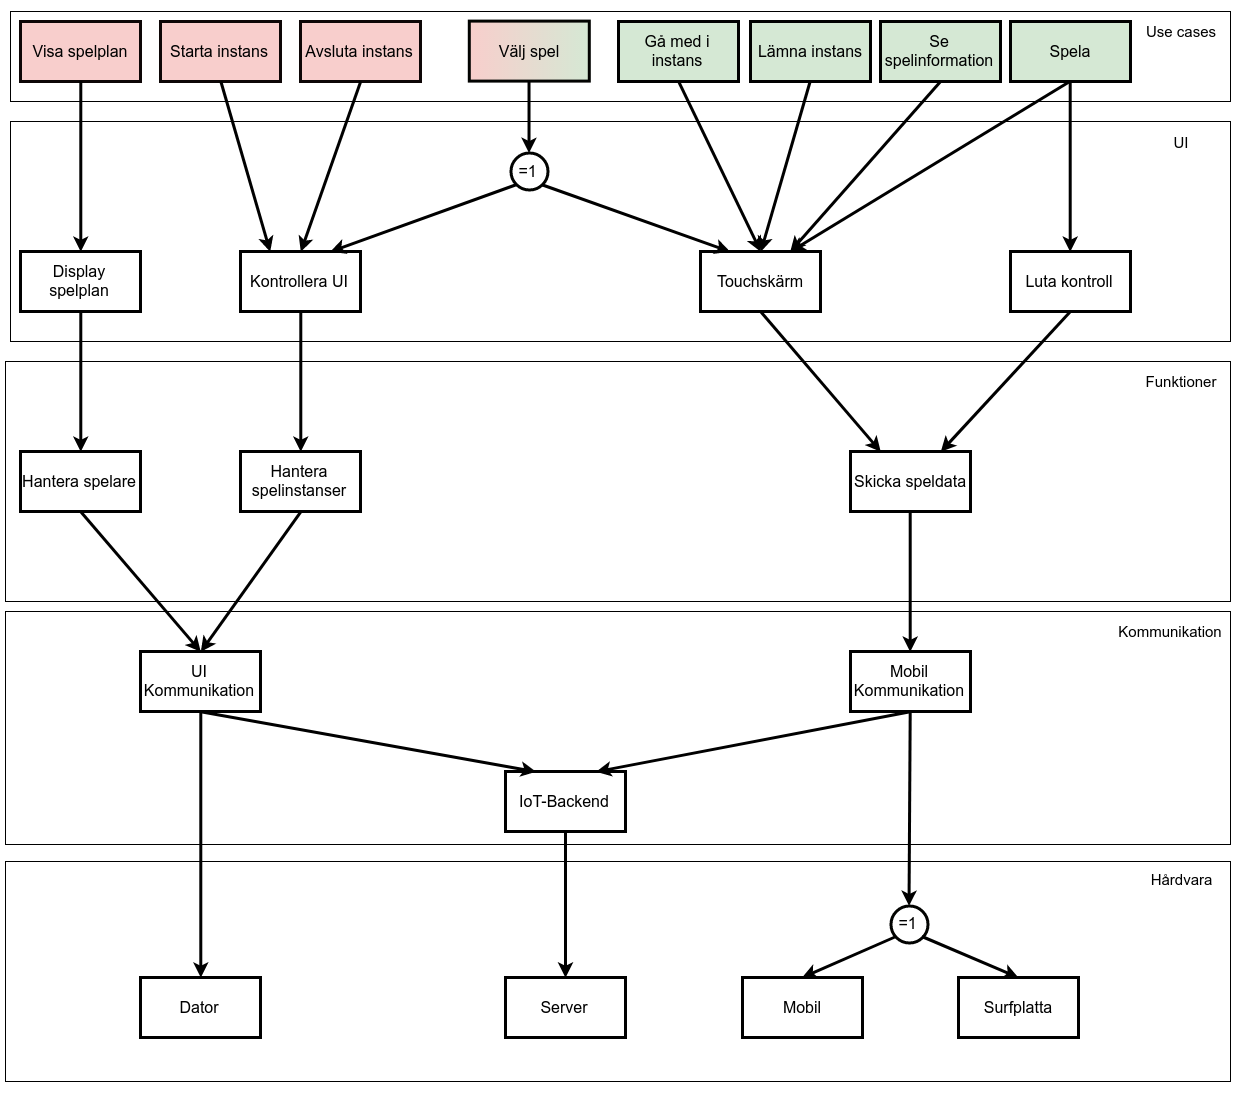
\includegraphics[scale=0.3]{systemanatomi_graf}
    \caption{Överblick av systemanatomin}
    \label{fig:systemanatomi_graf}
\end{figure}

\begin{figure}[H]
    \centering
    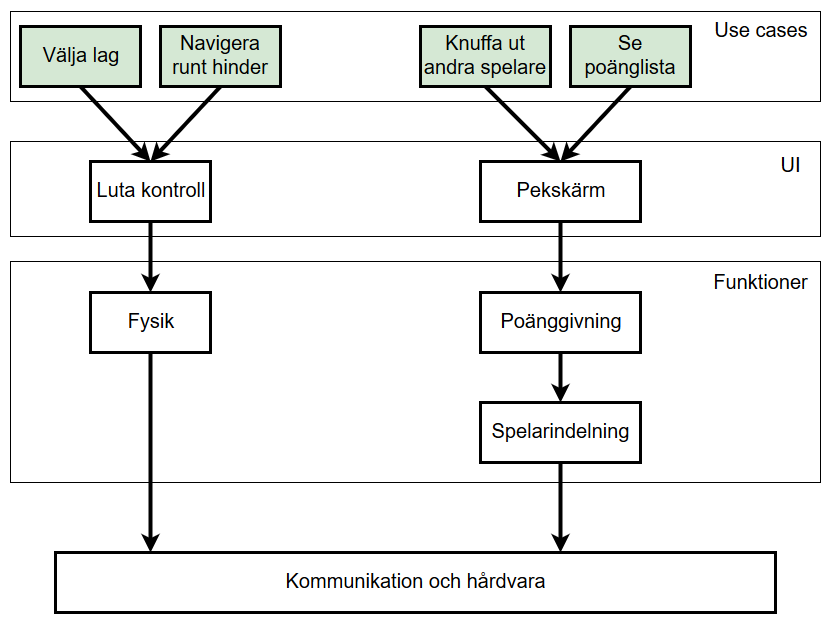
\includegraphics[scale=0.3]{systemanatomi_spel}
    \caption{Överblick av systemanatomin för spelet}
    \label{fig:systemanatomi_spel}
\end{figure}


\pagebreak

\subsection{Moduler}
\label{moduler}
Projektgruppen använde sig av den generella strukturen av systemet, kundens krav och systemanatomin för att skapa en mer detaljerad arkitektur. I figur \ref{fig:konceptarkitektur} kan man se den övergripande strukturen av modulerna som finns i applikationen.

\begin{figure}[h]
    \centering
    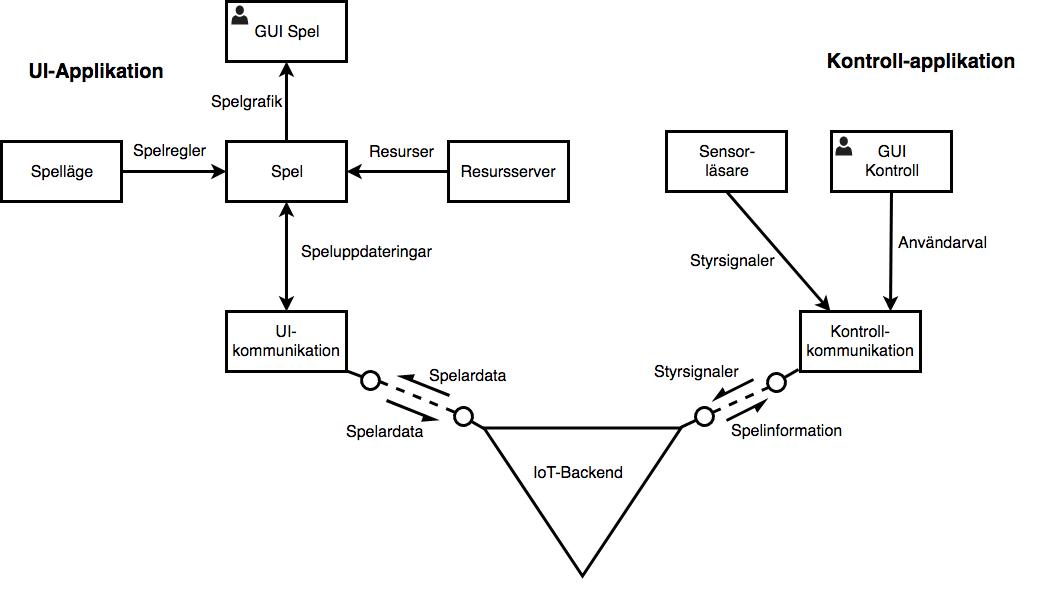
\includegraphics[scale=0.3]{konceptarkitektur}
    \caption{Överblick av systemets moduler}
    \label{fig:konceptarkitektur}
\end{figure}

\pagebreak


\subsubsection*{Ansvarsområden}
Varje modul i systemet har ett eget ansvarsområde. Nedan följer en förtydling på vad varje modul ansvarar för.

\begin{labeling}{\small{\textbf{Kontrollkommunikation}}}
    \item [\small{\textbf{GUI Spel}}]
        \begin{itemize}
            \item Visa upp spelplanen
            \item Visa upp menyer
            \item Starta spel med specifika inställningar
            \newline
        \end{itemize}

    \item [\small{\textbf{Spelläge}}]
        \begin{itemize}
            \item Sätta upp regler för spelet
            \item Avgöra vilka resurser spelet ska innehålla
            \item Avgöra vad som ska ske vid olika tillfällen i spelet
            \newline
        \end{itemize}

    \item [\small{\textbf{Spel}}]
        \begin{itemize}
            \item Hålla koll på de olika spelarna
            \item Tillhandahålla grundläggande spelmekanik
            \newline
        \end{itemize}

    \item [\small{\textbf{Resursserver}}]
        \begin{itemize}
            \item Lagra vilka resurser som finns
            \item Ladda in resurser
            \newline
        \end{itemize}

    \item [\small{\textbf{UI-kommunikation}}]
        \begin{itemize}
            \item Upprätta uppkoppling mot server
            \item Förpacka data för kommunikation
            \newline
        \end{itemize}

    \item [\small{\textbf{Sensorläsare}}]
        \begin{itemize}
            \item Läsa av data från sensor
            \item Abstrahera sensordata till standardiserad form
            \item Konfigurera sensor
            \newline
        \end{itemize}

    \item [\small{\textbf{GUI-kontroll}}]
        \begin{itemize}
            \item Visa menyer för att gå med i spelinstans
            \item Visa spelinformation om det pågående spelet
            \item Tillhandahålla knappar på skärmen
            \newline
        \end{itemize}

    \item [\small{\textbf{Kontrollkommunikation}}]
        \begin{itemize}
            \item Upprätta uppkoppling mot server
            \item Förpacka data för kommunikation
            \newline
        \end{itemize}

    \item [\small{\textbf{IoT-Backend}}]
        \begin{itemize}
            \item Dirigera data mellan olika Kontroll-applikationer och olika instanser av UI-applikationen
            \item Verifiera koder för att gå med i specifika spelinstanser
            \newline
        \end{itemize}
\end{labeling}


\section{Gemensamma erfarenheter}
Denna del tar upp diverse erfarenheter projektgruppen råkat ut för, både innan och under projektets gång.

\subsection{Erfarenheter av systemanatomi}
Systemanatomin som presenterades under \ref{beskrivning-systemanatomi} användes för att ge en enhetlig och helteckande bild över hur det färdiga systemet skulle se ut. Dock var arbetet med att ta fram själva systemanatomin något som tog relativt lång tid, om det vägs mot den nytta gruppen har haft av denna. Den blev mer ett verktyg som kunde användas för att verifiera resterande arkitekturbeskrivningar. Gruppen känner att själva processen att producera anatomin var nyttigare än den resulterande bilden, då det skapade en öppen dialog om systemets helhet.

\subsection{Tidigare erfarenheter}
Alla av projektets medlemmar hade studerat mer än två år på respektive program innan detta projekt startades. På grund av detta hade alla haft möjligheten att medverka i några större projekt och var därför ganska vana vid hur arbetet gick till. Dock var det få som hade erfarenhet med webbutveckling och spelprogrammering, något som hade stort fokus i detta projekt. Detta var dock inget större problem då de mer erfarna kunde hjälpa resten att komma igång.

\subsection{Nya erfarenheter}
Under projektets gång har alla medlemmar fått använda sig av nya verktyg och metoder som de inte haft tidigare erfarenhet av. De projektmedlemmar som tidigare saknade erfarenhet inom webbutveckling och spelprogrammering har fått chansen att sätta sig in i dessa. För att förbättra denna process hjälpte de som redan var erfarna inom ämnet till med att svara på frågor och komma med tips och idéer. Under projektets gång tillkom en del nya paket och ramverk. Ett exempel på detta är PIXI.JS, ramverket UI-applikationen använder för att rita ut spelet. Det var ingen i projektgruppen som hade jobbat med detta ramverk innan, så några i gruppen fick tillsammans sätta sig in i hur det fungerade och utbilda resterande vid behov. Detta gällde även en del av det olika npm-paketen som installerades och användes i projeket.


\subsection{Tidsbrist}
I början av projektet hade gruppen bra tidsplanering och lämnade in första iterationen i god tid för att sedan ta det lugnt. I början av iteration två satsade gruppen i huvudsak på utveckling och lämnade dokumentskrivning till senare, vilket visade sig vara en missbedömning. Detta ledde till att det blev stressigt framåt slutet av iteration två vilket kan ha påverkat dokumentkvaliteten negativt. Gruppen noterade dock detta och tog upp på kommande gruppmöten hur de skulle kunna göra det bättre inför kommande iterationer. Nästa iteration delades upp i en tydligare utvecklingsfas och dokumentfas, vilket tillät en bättre planering och fördelning av tiden.

\subsection{Tekniska erfarenheter}
Projektgruppen utvecklade applikationen i ramverket React som har något som kallas för states. Projektgruppen märkte att det snabbt kunde bli något rörigt när man introducerade flera lager av komponenter. Detta problem löser andra webbapplikationer genom extra verktyg för state-hantering, och gruppen reflekterade över dessa men beslutade emot att använda något liknande. Det visade sig dock i senare delen av projektet att hanteringen av states blev något rörig, då gruppen använt sig av fler komponenter än vad som först uppskattats. Detta ledde till att implementationen av nya komponenter som hamnade mellan redan existerande komponenter blev något jobbig. Detta berodde främst på att data som tidigare skickats från komponent \texttt{A} till \texttt{C} nu behövde skickas från \texttt{A} till \texttt{B} och sen vidare från \texttt{B} till \texttt{C}, när komponenten \texttt{B} introducerades mellan \texttt{A} och \texttt{C}. Detta ledde till att all data som tidigare skickades mellan \texttt{A} och \texttt{C} nu också behövde skickas till \texttt{B}, trots att det kunde vara data \texttt{B} inte använde sig av. En grafisk överblick kan ses i figur \ref{fig:middle_component}

\begin{figure}[H]
    \centering
    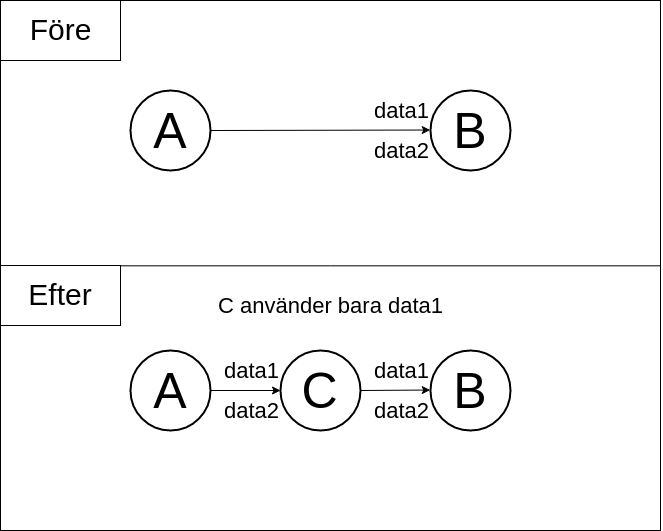
\includegraphics[scale=0.5]{middle_component}
    \caption{Överblick över hur implementation av mittenkomponent kan ge ett ineffektivt dataflöde}
    \label{fig:middle_component}
\end{figure}

\subsection{Erfarenheter med kundkontakt}
Under projekts gång har gruppen haft den stora nyttan av en nära kommunikation med kunden. Tidigt bjöds kunden in i en Slack-kanal med samtliga medlemmar, vilket ledde till en betydligt mer personlig kommunikationen än den som uppnås med mail. Gruppen har också utnyttjat kundens kontor och valt att arbeta där så mycket som möjligt. Då kunden uppmanade till att ställa frågor förtydligades diverse oklarheter snabbt vilket ledde till mer produktivt arbete. Den nära kundkontakten har också lett till en mer öppen dialog kring skapande och verifiering av produktkrav. I projektets början fördes en dialog kring krav tills kravspecifikationen ansågs vara tillräcklig. Under senare delen av projektet har kunden fått flera demonstrationer av produkten för verifiering av att den följer deras krav och vision.



%%%%%%%%%%%%%%%%%%%%%%%%%%%%%%%%%%%%%%%%%%%%%%%%%%%%%%%%%%%%%%%%%%%%%%
%%% lorem.tex ends here

%%% Local Variables:
%%% mode: latex
%%% TeX-master: "demothesis"
%%% End:

\chapter{Diskussion}
\label{cha:discussion}

I följande del presenteras olika tankar och idéer som uppkommit baserat på denna rapports innehåll och det genomförda projektet. De resultat som har uppnåtts väcker flera intressanta tankar och frågor. Det finns möjliga förbättringar till metoden som i efterhand har uppdagats. Arbetet existerar även i en samhällelig och etisk kontext som bör lyftas.

\section{Resultat}
\label{sec:discussion-results}

%Fanns alternativa implementationssätt?
Det fanns i det genomförda projektet många val som kunde leda till annorlunda resultat. Många teknikval har behövt tas för att färdigställa produkten. En stor andel av dessa har tagits enligt önskemål från kunden och det är inte troligt att kundens värde skulle kunna öka om dessa inte följdes. I denna kategori faller användning av React samt att koden skrevs i ren Javascript.

Många av de tekniska val som gruppen har tagit relaterar till speldelen av produkten. Ett stort sådant var att skapa spelet som ett mer allmänt ramverk för olika spellägen istället för ett specifikt spel. Det är troligt att projektet hade förändrats mycket om det andra alternativet hade valts. Då ett av kundens viktigaste önskemål var att enkelt kunna vidareutveckla projektet bedömdes dock det mer generella valet ge mer värde. Val av bibliotek för spelet var också ett viktigt avgörande i projektet. Flera alternativ diskuterades som till olika grad förlitade sig på färdiga paket för fysik, grafik och logik. Den slutgiltiga lösningen med PixiJS har givit stora möjligheter att skapa det system som önskades och gav även mycket stöd i rendering av spelets grafik. Utan färdiga bibliotek hade arbetet troligen tagit alldeles för lång tid. Användning av många stora bibliotek kan istället introducera oönskade begränsningar på projektets struktur.

%Vad återstår för att kunden skall få ut fullt värde av produkten?
Den slutgiltiga produkten innehåller några enkla spellägen som fungerar till fullo. Dessa kräver ingen vidareutveckling från kundens sida utan kan användas som tilltänkt efter leverans. Det är dock troligt att kunden vill introducera fler spellägen. En viss del av produktens värde ligger i hur hög utökningsbarhet som har uppnåtts för att underlätta denna process. Utförlig dokumentation har även skapats för att minimera tiden som krävs för att sätta sig in i systemet. Med detta är förhoppningen att skapandet av nya spellägen ska gå mycket smidigt och inte kräva förståelse för implementationsdetaljer.

%Lyckades ni förbättra/fortsätt något från tidigare projekt?

%Viktigaste lärdomar inför framtiden.

% Övrig mumbo-jumbo :S
Det fanns genom projektet en viss förvirring och osäkerhet gällande arbetet med systemanatomin. Ofta fanns stora skillnader i olika medlemmars uppfattning av hur anatomin skulle vara konstruerad. Det är möjligt att en otillräcklig förståelse för konceptet kan ha lett till att den framtagna modellen tappat mycket värde. Det är möjligt att svaret på frågeställning \ref{fs:fs_3} kunde haft ett större värde om det fanns fler ingående erfarenheter av arbete med systemanatomier. Gruppen diskuterade även huruvida relevansen av detta dokument kan förändras mycket mellan olika typer av projekt och utvecklingsmetodik. Det genomförda projektet befinner sig på en hög abstraktionsnivå med liten hårdvarukoppling. Det är av intresse hur systemanatomins nytta skulle se ut i mer hårdvarunära projekt, men detta har inte undersökts vidare.

Det är mycket troligt att resultat av projekterfarenheter har påverkats av att denna studie av processen har pågått parallellt. Gruppmedlemmarna har haft en medvetenhet om att projektet ligger till grund för detta arbete och även tagit del av seminarier som skapat en djupare reflektion. Detta delade fokus har troligen påverkat projektets utveckling. Det är dock troligt att utförandet av denna undersökningen parallellt är nödvändigt för att ge en tillräcklig insikt i projektet. Även om gruppens erfarenheter är att projektet ej kan anses till fullo representera typisk mjukvaruutveckling bedöms detta inte påverka resultaten i alltför stor utsträckning.

Testningen som gjorts under projektets gång har lämnat en lite önskande efter mer. De flesta test har utförts direkt efter koden som testats skrivits, och utav samma person och därmed inte varit en så utarbetad process man hade kunnat önskat. Detta berodde till stor del på avsaknad av ordentlig struktur från början och okunnighet från gruppens sida då få gruppmedlemmar var vana användare utav automatisk testning.

 En bit in i projektet började testningen komma ifatt och ett antal automatiska tester började formas. Möjligtvis blev testerna inte optimala då tidigare erfarenheter utav testning var bristande. En lärdom dras av detta att påbörja testningen i ett tidigare skede för att verkligen komma igång med det, kanske till och med testdriven utveckling \cite{TDD} vore ett bra alternativ. Om man formar produkten efter testerna blir man tvungen att skriva tester och får som en slags checklista att bocka av när testerna klarar sig. Dock hade det inte fungerat med vår nuvvarande setup då vi har en regel som säger att man inte kan synka med versionhanteringssystemet om test inte går igenom. 

Manuella tester är det som använts flitigast under projektets gång då manuella tester går snabbt och gruppen vet väl sedan tidigare hur de ska genomföras. De flesta har skett inofficiellt utav samma testare vilket kan vara en nackdel men utvecklingen har ändå gått framåt i en bra hastighet. Det finns ett par officiella tester \ref{fig:manual_test} som gjorts för att kolla så produkten lever upp till vad som är utlovat i kravspecifikationen. Dessa har gjorts utav en testare i samband med testledaren för att säkerställa att allting gått rätt till.

Då det ej fanns mycket utav tidigare kompetens inom testning skapade gruppen lite olika tester för att lära sig använda verktyget. Mycket upplärning skedde i början för att veta hur tester definieras och vad de gör. Det skapades olika sorters testning i syfte för att få bredare kunskap och få lärdom över vad de olika testerna faktiskt gjorde. Det användes allt från assertion testing\cite{assertion-testing} till snapshot testing\cite{snapshot-testing}.

Resultatet från den utförda enkätundersökningen uppnåde till stor del de önskade resultaten. Målet av undersökningen var att få ett snitt betyg över sex. Detta uppfylldes på alla frågor utom en, "Jag tycker det var svårt att förstå spelets regler", som fick betyget 5.8. Från att åtgärda detta problem implementerade gruppen en inforuta på både kontrollern och UI:t. Inforutan beskriver reglerna för spelläget som spelas. Enkätundersökningen utfördes inte ytterigare en gång efter inforutan hade implementerats. Detta hade varit intressant för att undersöka inforutans effekt på betyget. När medianen undersökts för de övriga resultaten syns det att detta resultatet är högre än medelvärdet. Detta tyder på att det var en större andel som röstade högt än lågt, men att de som röstade lågt, satte väldigt låga poäng.

% Are there anything in the results that stand out and need be
% analyzed and commented on? How do the results relate to the
% material covered in the theory chapter? What does the theory
% imply about the meaning of the results? For example, what
% does it mean that a certain system got a certain numeric value
% in a usability evaluation; how good or bad is it? Is there
% something in the results that is unexpected based on the
% literature review, or is everything as one would theoretically
% expect?

\section{Metod}
\label{sec:discussion-method}
%Vilka konsekvenser fick de valda metoderna för resultaten?
Den rolluppdelning som har gjorts har troligen påverkat delar av projektet och därmed resultatet. Rollerna har fört med sig dokumentationsbeslut och arbetsprocesser. Vissa ansvarsområden överlappar delvis och det är tänkbart att andra resultat hade nåtts om dessa hade slagits ihop till färre roller. Det finns även specifika roller som inte använts. Exempel på detta är tekniska experter över vissa områden i projektet. Denna sorts roll har i det utförda projektet till viss del uppstått spontant genom personer som är mer insatta i viss teknik. Det är möjligt att resultaten hade sett annorlunda ut om denna uppdelning hade skett i förtid och mer explicit.

%Fanns det alternativ?
Ett alternativ till den iterativa, agila arbetsmetodiken i projektet hade varit en mer traditionell vattenfallsmodell. Detta går dock mot gruppmedlemmarnas tidigare erfarenheter av problem med denna sorts arbetsprocess. Det skulle även finnas organisatoriska problem med detta utifrån planeringen av den kurs projektet ingår i. Denna jämförelse undersöks vidare i individuell rapport \ref{individual:lieth-wahid}. Även inom iterativa arbetsmetoder finns det olika alternativ som har övervägts. Istället för att basera arbetsmetodiken på Scrum skulle exempelvis Kanban\cite{kanban} eller Rational Unified Process\cite{RUP} kunnat användas.

Inom den variant av Scrum som har använts genom projektet finns många valmöjligheter som har förändrat utvecklingsprocessen. Längden på sprints, tid avsatt för vissa möten och uppdelning av arbetsuppgifter är saker som troligen har påverkat arbetet märkbart. Vilka delar av Scrum som har tagits med i projektets utförande har troligen också påverkat mycket. Exkludering av stand-up meetings är ett sådant centralt beslut. I det fallet ansågs det inte effektivt logistiskt. Här hade andra alternativ till daglig kommunikation kunnat övervägts för att uppnå samma effekter.

Arbetet med enkäterna och demonstrationerna påverkade troligen resultatet på helt olika sätt. Enkätundersökningen gjordes under projektets senare skede, under en tid då utvecklingsarbetets fokus var på kvalitet och inte funktioner. Alltså var det svårt för gruppen att använda sig av resultatet från denna undersökning på ett sätt som faktiskt visades i produkten. En möjlig förbättring på denna metod skulle vara att hålla flera enkätundersökningar under projektets gång och i sin tur använda sig av feedbacken i utvecklingsarbetet. Nu användes istället resultatet för att verifiera kvaliteten av en nästan färdigställd produkt. Detta skilde sig dock med demonstrationerna för kund. Denna feedback kom kontinuerligt under utvecklingsfaserna och feedbacken ledde till direkta ändringar av utvecklingen. En eventuell förbättring till denna metoden är att mer formellt dokumentera den feedback som gruppen får, för att senare verifiera dess påverkan på produkten.

%Källkritik.
En del av de använda källorna kommer från dokumentation över produkter skapade av företag. Här finns anledning att tro att ett visst intresse finns för att presentera dessa produkter med viss positiv vinkling. Dock har dessa källor endast används för tekniska specifikationer och i detta anses inte någon möjlig vinkling påverka korrektheten.

% This is where the applied method is discussed and criticized.
% Taking a self-critical stance to the method used is an
% important part of the scientific approach.
%
% A study is rarely perfect. There are almost always things one
% could have done differently if the study could be repeated or
% with extra resources. Go through the most important
% limitations with your method and discuss potential
% consequences for the results. Connect back to the method
% theory presented in the theory chapter. Refer explicitly to
% relevant sources.
%
% The discussion shall also demonstrate an awareness of methodological
% concepts such as replicability, reliability, and validity. The concept
% of replicability has already been discussed in the Method chapter
% (\ref{cha:method}). Reliability is a term for whether one can expect
% to get the same results if a study is repeated with the same method. A
% study with a high degree of reliability has a large probability of
% leading to similar results if repeated. The concept of validity is,
% somewhat simplified, concerned with whether a performed measurement
% actually measures what one thinks is being measured. A study with a
% high degree of validity thus has a high level of credibility. A
% discussion of these concepts must be transferred to the actual context
% of the study.
%
% The method discussion shall also contain a paragraph of
% source criticism. This is where the authors’ point of view on
% the use and selection of sources is described.
%
% In certain contexts it may be the case that the most relevant
% information for the study is not to be found in scientific
% literature but rather with individual software developers and
% open source projects. It must then be clearly stated that
% efforts have been made to gain access to this information,
% e.g. by direct communication with developers and/or through
% discussion forums, etc. Efforts must also be made to indicate
% the lack of relevant research literature. The precise manner
% of such investigations must be clearly specified in a method
% section. The paragraph on source criticism must critically
% discuss these approaches.
%
% Usually however, there are always relevant related research.
% If not about the actual research questions, there is certainly
% important information about the domain under study.

\section{Samhälleliga och etiska aspekter}
\label{sec:work-wider-context}

Projektet som har utvecklats har helt publicerats som open-source under licensen MIT\cite{MIT-license}. Detta är en mycket öppen licens som tillåter fri användning av programvaran för de flesta syften. Genom att dela med sig av all kod kan andra utvecklare välja att använda delar av den producerade koden i egna projekt eller lära sig av de designbeslut som tagits. Denna spridning av information och erfarenheter gör att mängden resurser för liknande framtida projekt ökar. Eftersom projektet är helt öppet och inte dolt bakom någon betaltjänst eller liknande hinder erbjuds alla samma möjlighet att ta del av det.

Projektet som har genomförts har från kundens sida syftet att demonstrera ett system för Internet of Things. Detta gör att projektet till viss del kan anses marknadsföra IoT som koncept. Direkta effekter av den utvecklade produkten på samhälle och miljö anses mycket små. Istället läggs här ett större fokus på indirekt påverkan från den mer uppkopplade värld som slutprodukten bidrar till att demonstrera.

%Samhälleliga
\subsection{Samhälle}
Introduktionen av IoT-koncept innebär stora förändringar av samhället. På en stor skala kan bussar och bilar tänkas vara uppkopplade mot servrar som kan erbjuda många logistiska optimeringsmöjligheter. Även i andra viktiga samhällsinstanser som sjukvård och räddningstjänst kan en mer uppkopplad värld erbjuda många möjligheter. På en mindre skala påverkar IoT varje enskild person och interaktionen mellan människor. Allt fler av objekten i vårt hem kopplas mot internet. Detta påverkar hur vi använder dessa och därmed våra levnadsmönster.

%Miljö
\subsection{Miljö}
Då fler och fler saker kopplas upp mot internet skapas nya behov av nätverk. Både i de uppkopplade apparaterna och i den kringliggande infrastrukturen krävs hårdvara som klarar av större mängder nätverkstrafik. Detta introducerar en ökad energianvändning på flera nivåer i nätverksstrukturen. Små objekt som tidigare innehållit ingen eller endast väldigt enkel elektronik behöver kunna upprätthålla nätverkskommunikation. Även behandling av de stora mängder data som kan skapas är en stor del av IoT-konceptet. Servrar som under lång tid utför tunga dataanalyser kräver stora mängder energi för att utföra sina uppgifter.

IoT erbjuder även många möjligheter för miljöarbete. Insamling av data genom många små sensorer och behandling av denna kan tänkas möjliggöra övervakning av processer som påverkar miljön. IoT tillåter också effektivisering av många industrier, vilket kan tänkas leda till en mer hållbar utveckling. Exempel på en industri med stor miljöpåverkan och möjligheter inom IoT är jordbruk. Här kan olika uppkopplade lösningar optimera resursanvändning och effektivisera processer, vilket ger en positiv miljöpåverkan.\cite{IoT-agriculture}

%Etiska
\subsection{Etik}
Med många små uppkopplade moduler skapas stora mängder data. Denna data har ofta en obetydlig natur i sig självt, men kan få värde i kombination med annan. I de fall denna data beskriver egenskaper hos personer eller deras aktiviteter introducerar detta flera etiska dilemman. Det blir aktuellt att ställa frågor om vem som äger datan och vad den får användas till. Många IoT-lösningar erbjuds som tjänster där all data lagras och hanteras på företags servrar. Det är då förståeligt att användare känner en viss oro för hur den används och sprids. Här läggs ett stort ansvar på företag och organisationer att ta fram riktlinjer för hur man behandlar denna data.

% There must be a section discussing ethical and societal
% aspects related to the work. This is important for the authors
% to demonstrate a professional maturity and also for achieving
% the education goals. If the work, for some reason, completely
% lacks a connection to ethical or societal aspects this must be
% explicitly stated and justified in the section Delimitations in
% the introduction chapter.
%
% In the discussion chapter, one must explicitly refer to sources
% relevant to the discussion.

\chapter{Slutsatser}
\label{cha:slutsatser}

Baserat på de uppnådda resultaten kan frågeställningarna svaras på i stor utsträckning. Det genomförda projektet kan därmed erbjuda vissa intressanta insikter enligt syftet med denna rapport. I följande stycken presenteras de slutsatser som har uppnåtts och arbetets vidare lärdomar.

\section{Frågeställningar}

\subsection*{\ref{fs:fs_1} Hur kan ett realtidsspel som använder sig av Cybercoms backend implementeras så att man skapar värde för kunden?}

Ett system baserat runt Cybercoms backend har implementerats. Systemet består av ett spel med flera olika spellägen. Speciellt arbete har lagts på att försäkra sig om att spelet känns responsivt för användarna. Detta ger kunden värde då det demonstrerar effektiviteten i den existerande backenden.
Med möjligheten att skapa nya spellägen finns stor potential till vidareutveckling av produkten. Detta ger kunden stort värde för framtida användning av systemet.

\subsection*{\ref{fs:fs_2} Vilka erfarenheter kan dokumenteras från programvaruprojektet som kan vara intressanta för framtida projekt?}

En organisatorisk erfarenhet som kan tas med från projektet är hur mjukvaruutveckling och dokumentskrivning kan balanseras. Att arbeta mer kontinuerligt och parallellt med dokument och kod i projekt har visat sig fördelaktigt. På den tekniska sidan finns flera erfarenheter av React-utveckling. En stor sådan är vikten av att organisera lager av komponenter. React har visat sig lätt introducera problem med rörig kod då inga verktyg för state-hantering används.

\subsection*{\ref{fs:fs_3} Vilket stöd kan man få genom att skapa och följa upp en systemanatomi?}

En systemanatomi kan erbjuda viss hjälp med att ge en översiktlig bild över ett system. I en grupp kan den även bidra till en mer gemensam bild av vad som ska skapas och därmed förhindra missförstånd. Att ta fram systemanatomin har dock visat sig vara en svår process. I det utförda projektet upplevdes det svårt att få en gemensam bild över vad systemanatomin representerar. Det är troligt att detta har reducerat det stöd som gruppen har fått av modellen.

\subsection*{\ref{fs:fs_4} Hur kan kontinuerliga användardemonstrationer användas i utvecklingsfasen för att förbättra ett spels kvalitet?}

I det utförda projektet har spelet flera gånger demonstrerats för kunden. Dessa demonstrationer har använts som kontroller över att utvecklingen går i rätt riktning. De har även varit möjligheter för kunden att förtydliga eller justera sina mål med projektet. Idéer till olika lösningar har också kunnat diskuterats öppet.

\section{Måluppfyllelse}

Det genomförda projektet har till stor del lyckats skapa värde för kunden. Det slutgiltiga systemet demonstrerar flera kvalitetsaspekter hos kundens IoT-backend. Spelet erbjuder också goda möjligheter till vidareutveckling genom nya spellägen. Slutprodukten anses därför väsentligen ha uppfyllt de mål som projektet utgått från.

Denna rapport ger en god bild över den utvecklingsprocess som har följts och resultaten från utvecklingsarbetet. Genom erfarenheter och reflektioner från det utförda projektet har de presenterade frågeställningarna kunnat svarats på. Med avseende på projektets storlek anses dessa slutsatser vara av god relevans. För ytterligare generella aspekter av frågeställningarna skulle troligen flera olika projekt behöva studeras, men detta ligger utanför detta arbete.

\section{Viktiga insikter}

Från detta arbete finns flera intressanta insikter om både teknisk implementation och utvecklingsprocessen. Det utförda projektet presenterar en möjlig variant av agil utveckling som kan ge en värdefull slutprodukt. Detta visar att en mer avskalad variant av ett utvecklingsramverk som Scrum kan passa bra för projekt av mindre skala.

Många dokument har producerats i projektet och skapat stöd för gruppmedlemmarna. Dessa dokument har på olika sätt kommit till nytta innan, under och efter utvecklingsarbetet. Värdet hos olika sorters dokument är en nyttig insikt från det utförda projektet. Speciellt har det reflekterats över användning av systemanatomier. Denna typ av dokument, som till viss del skiljer sig från många andra systemmodeller, kan vara ett nyttigt verktyg att ta med sig till framtida projekt.

% This chapter contains a summarization of the purpose and the research
% questions. To what extent has the aim been achieved, and what are the
% answers to the research questions?
%
% The consequences for the target audience (and possibly for researchers
% and practitioners) must also be described. There should be a section
% on future work where ideas for continued work are described. If the
% conclusion chapter contains such a section, the ideas described
% therein must be concrete and well thought through.

\chapter{Översikt över individuella delar}
Projektgruppens medlemmar har utfört mindre undersökningar av specifika aspekter hos projektet. Dessa presenteras som bilagor till denna rapport. Nedan följer korta introduktioner till de olika undersökningarna.

\subsection*{\fullref{individual:joel_a}}
Teamet utförde ett större projekt på 3200 arbetstimmar, under detta projekt så undersöktes många saker för att skapa en så bra produkten som möjligt. Men en aspekt som inte undersöktes var den miljömässiga som inte ställdes som krav av varken kunden eller teamet. Denna rapport försöker uppskatta hur mycket koldioxid som gruppen släppt ut under sin utvecklingsprocess och vad som skulle kunna ha gjorts för att minska denna siffra.

\subsection*{\fullref{individual:bjorn}}
Versionshantering är en viktig del av modern mjukvaruutveckling. Under de senaste tio åren så har det dykit upp många nya verktyg, tjänster och metoder. Borde man ha centraliserad eller decentraliserad? Hur ska man förgrena? Det finns mångra frågor och ännu fler svar. Genom att studera rapporter, artiklar och statistik försöker rapporten sammanställa de populäraste alternativen och dra några slutsatser om när de är lämpligast.

\subsection*{\fullref{individual:tim}}
IoT är ett koncept som har stor utbredning i vårt samhälle idag. Med detta behövs bra algoritmer och strukturer för att skicka och hantera data mellan en stor mängd enheter. Deepstream är en tjänst som erbjuder kommunikation samt hantering av data i realtid. I denna delen av rapporten granskas då denna tjänsten genom att göra en undersökning av hur deepstream serialisera sin data för minska nätverksbelastning och hur detta påverkar rundturstider. Efter att ha undersökt tjänsten så visade det sig att deepstream inte gör någon speciell serialisering utan skickar JSON-objekt i läsbart format. Dessutom såg man att RPC gick något snabbare att exekvera gentemot events, men att båda växer linjärt med datastorleken.

\subsection*{\fullref{individual:david}}
Testning är något som alla vet är ett ont måste. Men måste det vara en utdragen process som man bara behöver få avklarad? Det den här studien kommer gå in djupare på är en undersökning i automatiska tester, speltestning och hur de lite mer knepiga testerna går till. Fördjupningen kommer ligga i Jest då det kommer grundas i många egna erfarenheter, men det kommer dras paralleller mellan olika testverktyg som Jasmine och Mocha. Jämförelser kommer göras som diskuterar skillnader mellan verktyg, vad som är grundläggande inom testvärlden och hur man kan få ut det mesta ur sina tester. De jämförda verktygen visar sig dock inte innehålla några stora skillnader, utan det kommer mer ner till vad man känner sig bekväm med för vilket syntax, där vissa verktyg har lite mer kött på benen gällande vilka bibliotek man använder sig utav i Javascript.

\subsection*{\fullref{individual:axel}}
Utvecklingen av webbapplikationer har genom gått stora förändringar på bara de senaste 10 åren. Flera nya ramverk och bibliotek har introducerats för att underlätta utvecklingsprocessen. En konsekvens av detta är att det har blivit svårare för en utvecklare att bestämma vilket ramverk eller bibliotek lämpar sig bäst för sin webbapplikation. I denna delen av rapporten jämförs de två mest populära verktygen, React och Angular. Rapporten fokuserar på hur lätt det är för en utomstående utvecklare att bidra till ett projekt och jämför även strukturella skillnader. Baserat på erfarenheter som samlats från projektet, diskuteras att React passade bättre för det utförda projektet. Resultaten visar på att React är ett lättare verktyg att lära sig men att Angular har en tydligare struktur för något ska implementeras. Resultatet visar även på att Angular är ett lämpligare verktyg för större project medan React lämpas mer för mindre projekt, då användbarhet sätts i fokus.

\subsection*{\fullref{individual:joel_o}}
Stora ekosystem av färdigskrivna paket med mjukvara har på senare år nått stor popularitet. Det största arkivet av sådana paket är npm för Javascript. I detta arbete undersöks hur beroenden till färdiga paket påverkar utvecklingsprocessen och kvalitet hos slutprodukten för mjukvara skriven i Javascript. En kvantitativ analys av över 6~000 populära Javascript-projekt har utförts för att ta reda på hur utbredd denna praxis är. Resultaten från analysen visar att de undersökta Javascript-projekten i genomsnitt har 6.76 direkta beroenden. Baserat på projekterfarenheter presenteras också hur beroenden kan förändra mjukvaruutvecklingsprocessen. Slutsatser dras även om hur beroenden bör hanteras för att maximera säkerhet och tillförlitlighet hos ett system.

\subsection*{\fullref{individual:alexander}}
Javascript, det primära programmeringsspråket gruppen utvecklat i, är ett dynamiskt typat språk avsätt för webbprogrammering. Den dynamiska typningen språket har leder till en mer uttrycksfull programmeringsupplevelse. Men hur påverkar egentligen den dynamiska typningen utvecklingsarbete i språket, och hur står det sig mot strikt typade alternativ som Facebooks Flow eller Microsofts Typescript? Undersökningen i denna del använder sig av forskning från tidigare studier för att bestämma detta, tillsammans med projektgruppens egna erfarenheter i Javascript. Resultatet från undersökningen pekar mot att utveckling i ett typat alternativ leder till färre publika buggar och reducerad utvecklingstid.

\subsection*{\fullref{individual:lieth-wahid}}
Dagens arbetsmarknad kräver ingenjörer som kan tillämpa teorin som de har lärt sig under sina högskolestudier i praktiken. För att förbereda sådana ingenjörer måste man ha hänsyn till utvecklingsmetodiken som används under studietiden. Vattenfall är det mest använda utvecklingsmetodiken i projektbaserade kurser inom mjukvaruutveckling som ges vid högskolestudier. Scrum, å andra sidan, är ett ramverk som är väldigt populärt inom agil utveckling. Metoden har börjat används vid fler universitet runt om världen. Både metoder har sina för-och nackdelar. Denna undersökning jämför vattenfall arbetsmetoden med Scrum och diskutera vilken är mer fördelaktig för studentprojekt. Undersökning använder sig av rundfrågor samt ett frågeformulär på en studentgrupp som består av åtta studenter. Resultatet från undersökningen visar att en kombination av både metoden skulle vara mer fördelaktig för studentprojekt.

\appendix

\chapter{Tekniker för responsitivitet av Björn Detterfelt}

\section{Introduktion}
\label{sec:bjorn-introduction}

Den här rapportens syfte är att undersöka hur versionshantering kan användas tillsammans med agila uvecklingsmetoder. Rapporten kommer att fokusera till stor del på den information som finns tillgänglig online och de erfarenheter och debatter som går att finna.

\subsection{Motivering}
\label{subsec:motivation}

Versionshantering är inte ett krav för att kunna arbeta agilt men det kan göra det lättare. Det är också ett kraftfullt verktyg för samarbete inom open-source projekt men också för teambaserad produktutveckling. Dock så finns det inte bara ett sätt att versionshantera på, vilket kan ge upphov till oklarheter när det ska versionshanteras. Därför undersöker rapporten populära alternativ och i vilka situationer de kan vara bäst att använda.

\subsection{Syfte}
\label{subsec:reason}
Den här rapportens syfte är att undersöka vilka moderna alternativ som finns för versionshantering med fokus på hur de lämpar sig för agil utveckling.

\subsection{Frågeställning}
\label{subsec:research-questions}

För att uppfylla syftet så kommer rapporten baseras på följande frågeställningar:

\begin{enumerate}
\item Vilka arbetsmetoder finns för att åstadkomma effektiv agil versionshantering?

\item Hur skiljer sig de olika populära versionshanteringssystemen?
\end{enumerate}


%    Does this workflow scale with team size?
%    Is it easy to undo mistakes and errors with this workflow?
%    Does this workflow impose any new unnecessary cognitive overhead to the team?


\subsection{Avgränsningar}
\label{subsec:delimitations}

Undersökningen begränsas till populära metoder till verktygen Git, Subversion och Mercurial samt information som är närliggande i tid.
\section{Bakgrund}
\label{sec:bjorn-background}

Git är ett kraftfullt versionshanterings verktyg som har blivit väldigt populärt att använda inom industrin. Samtidigt har även agila utvecklingsmetoder vuxit fram. Git lämnar stor frihet till utvecklarna att välja hur det ska användas. Den agila filosofin lämnar också stora friheter. Tillsammans ger det upphov till oklarheter om hur Git bäst kan användas till Agila utvecklingsmetoder.

\subsection{Git}

\subsection{Agila filosofin}
\section{Teori}
\label{sec:bjorn-theory}
De grundläggande koncepten för rapporten defineras och förklaras i det här kapitlet.

\subsection{Git}
Git är ett distribuerat versionshanteringsverktyg. Det skapades ursprungligen av Linus Torvalds för att täcka behoven till utvecklingen av Linux efter att deras dåvarande versionshanteringsverktyg BitKeeper tog bort deras gratisklient. Git skapades med krav på att den skulle vara distribuerad och snabb samt ha ett skydd mot korruptering. Git släpptes först i december 2005 och har sedan varit i konstant utveckling och förbättring \ref{linux-google} När Git släpptes var SVN dominerande och Git skiljde sig åt på många sätt, främst genom den distribuerade modellen. Det tog ett par åt innan Git började bli populärt men sedan dess har Git vuxit i popularitet med rasande fart och är idag det populäraste versionshanteringsverktyget. Git används i nuläget för både enorma projekt som Windows och Linux men också för små hobby projekt.\ref{vcs-popularity}
Exempel på de största fördelarna med Git är att det finns starkt stöd för förgrenande utveckling där det bland annat är lätt att sedan kombinera ihop grenar av kodbasen i en så kallad merge. Ett kraftigt verktyg som finns till hjälp där är en så kallad pull-request som tillåter att koden kan granskas och testas innan man utför en merge.\ref{pull-request} En annan fördel som kommer från att den är distribuerad gör så att det blir enklare för utvecklare att utveckla lokalt och ger bättre verktyg för att gå bakåt i historiken eller utföra en merge lättare.

\subsection{Mercurial (hg)}
Mercurial är liksom Git ett distribuerat versionshanteringsverktyg som skapades av samma anledning med tanke att bli det nya versionshanteringssystemet för Linux utveckling. Trots att Git användes istället så fortsattes Mercurial att utvecklas och har sett en del använding inom open-source projekt som Netbeans\ref{netbeans-contribute} men också utav stora företag som Facebook\ref{facebook-mercurial}.
Mercurial är på många sätt väldigt likt Git i hur det fungerar men har fördelar som att kommandon är simplare och har bättre koll på specifik historik för en viss fil. En annan fördel är att den är lättare att utöka med egen funktionalitet.\ref{mercurial-book}

\subsection{Subversion (SVN)}
SVN är ett centraliserat versionshanteringsverktyg. Det skapades år 2000 med syfte av att vara en bättre version av den då populära CVS och det fanns ursprungligen inga tankar på att revolutionera versionshantering. Därmed blev det ett logiskt och simpelt val för användare av CVS att byta över till SVN då SVN fungerade ekvivalent eller bättre. Efter att SVN blev populärt så har den vidareutvecklats och används fortfarande av många företag\ref{vcs-popularity} och open source projekt som The Apache Software Foundation\ref{apache-dev-svn}.\ref{svn-book}

\subsection{Agila utvecklingsmetoder}
Agila utvecklingsmetoder handlar om att värdera flexibilitet och samarbete över de traditionella värdena som planer och processer. De menar inte att de traditionella värdena är meningslösa utan att de är värdefulla, men det är värdefullare att kunna jobba närmare kunden och att våga ändra på planer under projektets gång. Agila utvecklingsmetoder siktar på att produkten utvecklas i kortare perioder där man låter kunden få säga till om vad de vill. Det agila arbetssättet förespråkar att utvecklarna skriver väldigt lite dokumentation och istället mycket kod så att ifall kunden ändrar sig så har man inte lagt tid på att dokumentera onödiga saker. Det kan dock göra det svårare för nya utvecklare att sätta sig in i ett projekt.
Det finns många väl sätt att utveckla agilt på och några populära metoder är Scrum, Kanban och Extreme Programming.
\section{Metod}
\label{sec:bjorn-method}

Det utvecklas hela tiden nya metoder för versionshantering och de metoder som finns vidareutvecklas. Problem som nämns i källor som bara är några år gamla kan vara fixade eller lösta genom nya arbetssätt. Därför läggs större vikt på nya källor för att få en bättre bild av hur versionshantering fungerar i dagsläget. På grund av det finns det ont om relevanta rapporter att studera och en stor del av det studerade materialet blir artiklar och bloggar.
\section{Resultat}
\label{sec:bjorn-results}
Här sammanställs kvalitativ information från de resurser som erfanns.

%Projektet:
%Feature branching, CI, Code reviews, Squashing
%Historik försvinner, svår blame

\subsection{Undersökning}
Enligt Atlassians jämförelse av centraliserade och distribuerade versionshanteringssystem kan man emulera centraliserade system med distribuerade. Genom att välja ett distribuerat system som Mercurial eller Git får man då tillgång till samma arbetsflöden som centraliserade system erbjuder samtidigt som man får de fördelarna som ett distribuerat system ger. Som sammanfattning ger de följande fördelar:
\begin{enumerate}
\item De flesta aktiviteter blir väldigt snabba då de kan utföras lokalt.
\item Det går att lagra ändringar utan bekymmer.
\item Ändringar kan delas, testas och diskuteras utan att skapa problem för andra utvecklare.
\end{enumerate}
Dock så blir man av med de fördelar som kommer av att lagra historiken på en centraliserad server, det vill säga att det kan bli problem med diskutrymme i projekt med väldigt många filer och mycket historik.\cite{central-vs-distributed}

Atlassian rekommenderar arbetsflödet "feature branching" för agila team. Feature branching bygger på att det finns en stabil huvudbranch som fungerar och att all ny funktionalitet utvecklas på egna brancher som utgår från huvudbranchen. Det här arbetsflödet passar bra ihop med popullära agila metoder som Scrum och Kanban genom att man skapar en branch för varje uppgift. Feature branching kombineras också ofta med den agila processen Continuous integration (CI) som innebär att man integrar ny funktionalitet så fort den är redo och använder automatiska tester. Den kombineras också med kodgranskning som ger möjlighet för andra utvecklare att ge feedback. Målet med de processerna är att minimera tiden som måste läggas på att kombinera utvecklingen från två branches och se till att huvudbranchen håller bra kvalité enom att koden granskas och testas.\cite{daly-agile-git, radigan-feature-branch, atlassian-feature-branch}

Martin Fowler tar upp några problem med feature branching och CI i sin webinar. Han beskriver att ofta fungerar det bra så länge det bara byggs nya features. Däremot så kan det uppstå stora problem när det sker stora ändringar utav den existerande koden, till exempel när det har utförts en omfaktorering. När omfaktoreringen ska slås ihop med huvudbranchen måste all kod som hamnat på huvudbranchen medans omfaktoreringen utfördes också omfaktoreras. Det kan vara tidskrävande då det kan vara svårt att hitta all användning av den omfaktorerade koden och det finns inget direkt stöd från versionshanteringssystemen förrutom förmågan att se de ändringar till huvudbranchen som hänt. När det är gjort och omfaktoreringen hamnat på huvudbranchen så blir det problem på alla branches som varit i utveckling parallelt då utvecklarna måste spendera tid på att uppdatera koden i deras branches.
Som en lösning på det här problemet föreslår han en variant av CI som han kallar Promiscuous Integration (PI). Den tar fördel av de distribuerade systemen och innebär att man integrerar mellan brancher direkt när man vet att det kommer ske stora förändringar eller när båda brancher utvecklar liknande funktionalitet så att de kan samarbeta. PI är inte perfekt och kräver att utvecklare pratar med varandra om vad de håller på med. Det ingår det i de flesta agila arbetsmetoder men kan vara problematiskt när man jobbar med utspridda teams. Det kan också göra det rörigt med att hålla koll på vilken funktionalitet som finns på vilken branch men för det mesta kan versionshanteringssystemen effektivt hjälpa till med det.\cite{fowler-feature-branch}

%git workflows:
%centralized - rebase istället för merge gör det lättare att se var buggar kom ifrån
%feature branch! - continous integration, testning
%gitflow
%forking

%korta branches
%enkla reverts
%matcha release cykeln

När kod ska kombineras så sker det oftast inga problem som inte kan lösas automatiskt av versionshanteringsvektygen när ett effektivt arbetsflöde följs. Men det förekommer ändå tillräckligt ofta problem som behöver lösas manuellt för att det ska vara intressant att studera hur de borde lösas. För att effektivast lösa de "merge conflicts" som uppstår när kod från olika brancher ska kombineras så är det viktigt att de som skrivit koden är involverade. Det är också hjälpsamt om koden är förstålig och om de verktyg som används visar bra information.\cite{8094445}

Kodgranskning är en viktig del av de flesta agila utvecklingsmetoderna och versionshanteringsverktygen hjälper genom att visa de förändringar som skett i koden. Moderna kodgranskningar är baserade till stor del på att titta på vad versionshanteringsverktygen visar. Sättet som förändringarna visas på kan påverka kvalitén av kodgranskningen. En nyligen utförd studie fann att den optimala ordningen att visa ändringarna på borde baseras på hur de relaterar till varandra. \cite{8094433}
\section{Diskussion}
\label{sec:bjorn-discussion}

Diskussion om ovanstående.

\subsection{Resultat}
\label{subsec:bjorn-discussion-results}

Analys av resultatet.

\subsection{Metod}
\label{subsec:bjorn-discussion-method}

Diskussion om metoden, kritik till vald metod etc.

\section{Slutsatser}
\label{sec:bjorn-conclusion}



\chapter{Deepstream serialisering och rundturstid av Tim Håkansson}

\section{Introduktion}

Under de senaste åren så har allt fler och fler enheter blivit inkopplade i IoT ekosystemet och än så länge ser det ut att fortsätta frammåt med hela 24 miljarder förväntade enheter uppkopplade\cite{IoT-ecosystem}. För att realisera denna utvecklingen behövs det robusta lösningar som klarar av att hantera, lagra och slussa data i realtid, samtidigt som lösningen behöver vara enormt skalbart. Det är här tjänsten deepstream\cite{deepstream} kommer in i bilden. Tjänsten annonserar sig att vara en snabb, enkel och säker tjänst som sedan 2015 börjat komma upp lite här och där. Deepstream används i ett flertal olika tjänster, med de mest noterbara briteback och ticketmaster\cite{ds-usecases}.

Projektet, som pappret utgår ifrån, utfördes under vårterminen 2018 och använde sig utav deepstream för att skicka, ta emot och hantera data. Anledningen till just deepstream var att våran kund, Cybercom, använde sig av denna tjänsten under sin utveckling av IoT lösningar. Eftersom deepstream annonserar sig att vara en kraftfull server som klarar av att hantera data mellan olika enheter i realtid, så finns det en motivering att undersöka hur väl det anpassar sig in i spelvärlden, där responsivitet för indata är a och o.

\subsection{Syfte}
\label{subsec:tim-aim}
Projektet som har utförts bygger en hel del på att nätverkslösningen som implementerats är snabb och skalbar för att uppnå maximal responsivitet för många användare. För att uppnå detta krävs en djupare förståelse för hur deepstream hanterar data beroende på olika inverkningar i systemet. Inverkningarna som tas upp i detta pappret är belastning, datastorlek och hur biblioteket används (gällande RPC gentemot event).

Genom att då undersöka dessa förhållanden kan teamet ta lärdom av hur data ska hanteras och när och hur data ska skickas.

\subsection{Frågeställning}
\label{subsec:tim-research-questions}
För att göra denna undersökninen krävs några fundementala frågor som behöver besvaras, dessa presenteras nedan:

\begin{enumerate}
\item Hur påverkas responsiviteten i nätverket beroende på datastorleken?  

\item Under vilka förhållanden är det bättre att använda RPC över event och vise versa?

\item Lämpar det sig att använda sig av deepstream för att hantera indata i ett realtidsspel?

\end{enumerate}
\subsection{Avgränsingar}
\label{subsec:tim-delimitations}
Då det inte går att deligera hur mycket tid och resurser som helst på undersökningen behöver vissa avgränsningar göras. Till en början så undersöks inte deepstream i en verklig miljö, dvs undersökningen görs på ett lokalt nätverk. Detta leder till att responstiderna till stor del inte reflektera rundturstiden (RTT) för nätverket då all data skickas på ett lokalt nätverk.

Dessutom så kommer inte responstiderna ta skalbarheten in i beräkningen då resurser för att koppla upp ett stort antal användare inte finns tillgängligt. Så responstiderna är endast med avseende på ett tomt nätverk och därmed handlar det mer om hur snabbt deepstream kan arbeta med datan innan den skicka datan vidare.

I pappret hanteras inte heller deepstreams records då denna strukturen inte är relevant för projektet.

\section{Bakgrund}
\label{sec:tim-background}
När det gäller datakomprimering så finns det andra studier som har gjorts som analyserat serialisering och deserialisering för olika typer av datastrukturer. I ''Performance Evaluation of Object Serialization Libraries inXML, JSON and Binary formats'' skriven av Kazuaki studerades olika data format, JSON, XML och binära format och hur dessa förhåller sig till varandra. Detta gäller datastorlek och hastighet för serialisering och deserialisering. Utöver det så granskas även olika bibliotek för samma format, där alla körs i Java. Detta för att få en bredare syn på hur formatet påverka exekveringstiden och inte hur väloptimerat biblioteket är. Resultatet från studien visar att binär data generellt sätt är snabbare och mer komprimerat i alla fall.

\section{Teori}

\label{sec:tim-theory}
För att göra undersökningen behövs en viss grund av begrepp och teminologier fastställas för att underlätta arbetet i senare skedde.

\subsection{JSON}
JSON\cite{json} är ett dataformat för att lätt kunna hantera data, både för en dator och en användare. Formattet bygger översiktligt på fält med värden, objekt med flera fält och listor med objekt. Men listor kan även finnas i objekt och listor kan också innehålla fält. Formatteringen kan se ut som i figur \ref{fig:jsonformat} där det finns ett objekt med en lista av anställda.

\lstset{language=Java}
\begin{figure}[h]
  \begin{minipage}[c]{5cm}
    \begin{lstlisting}
{
    "name": "John",
    "age": 30,
    "cars": {
        "car1": "Ford",
        "car2": "BMW",
        "car3": "Fiat"
    }
} 
    \end{lstlisting}
  \caption{JSON formattering}
  \label{fig:tim-jsonformat}
  \end{minipage}
\end{figure}

\subsection{Deepstream}
\label{subsec:tim-deepstream}
Deepstream är en Javascript-baserad tjänst med skalbarhet och datahantering i realtid i åtanke. Saker som utmärker detta gränssnitt är dess realtidsdatabaser, autentisering och behöver ingen backend utveckling för att fungera. För att få en fungerande backend behöver man endast starta en deepstream server och sedan är allt igång. Resten av integreringen sker på klientsidan av applikationen, så all datahantering sker utan någon form av serverprogrammering. För att få denna moduläriteten hanteras all data av servern med hjälp av tre enkla koncept. Dessa koncept är records, events och RPCs (Remove Procedure Call) och beskrivs mer ingående nedan. 

\subsubsection{Deepstream record}
Idén med records är att kunna lagra, updatera och ta bort data utan att denna datan försvinner efter körning. Detta samtidigt som att datan ska vara synkroniserad mellan alla uppkopplade enheter. För att uppnå detta använder deepstream en databas server som kan konfigueras till att hantera Postgres, MongoDB, ElasticSearch eller RethinkDB. 

Då detta pappret inte kommer hantera records så kommer ingen mer ingående förklaring ges\cite{ds-storingdata}.

\subsubsection{Deepstream event}
Ett event (även kallad kanal) kan ses som en direkt länk mellan flera publicerare och prenumeranter. En publicerare är helt enkelt en användare som skickar data till deepstream server via en viss kanal som ges av en sträng (vanligtvis med format ''projekt/kanalnamn''). När deepstream servern mottagit datan skickas den vidare till alla användare som prenumerera på samma kanal. 

Datan som skickas är i JSON-format och kommer inte lagras på deepstream servern. Därmed är tanken med events att det ska vara snabbt och enkelt att skicka data. 

\subsubsection{Deepstream RPC}
Utifrån events och records behövs det något enkelt sätt att skicka data samt få ett svar på den skickade datan. Detta kan vara ett enkelt fall då man implementera en addition RPC på en client och anropa den från en annan för att få ett svar på beräkningen. Detta är ett av de mest triviala exemplet, men all form av validering, beräkning eller liknande som man vill göra på en annan klient görs enklast med hjälp utav RPCs.

På samma sätt som i events så skickas datan i ett JSON-format, både för anropp och svaret från RPCn.

\subsection{Rundturstid}
När rundturstid nämns i denna delen av pappret menas tiden det tar att skicka en förfrågan till en annan klient i nätverket och få tillbaka ett svar. Det vill säga tiden det tar att skicka ett meddelande till deepstream servern, få servern att skicka vidare till en annan klient som sedan skicka tillbaka ett svar genom servern. Det betyder \textbf{inte} tiden det tar att få ett direkt svar från deepstream servern då detta inte ger ett relevant värde eftersom att klienter aldrig kommunicera direkt med servern.

\subsection{Wireshark}
Wireshark är ett verktyg för att analysera nätverkstrafik för att se över vad som skickas, över vilket protokol och vem som skicka eller tar emot datan. Detta ger användaren en bra förståelse för hur olika protokol fungera på en lägre nivå.

\subsubsection{Interface}
Utifrån det kan man ställa in vilket interface\cite[p.~364]{networking} man lyssnar på, detta inkluderar generellt bluetooth, ethernet och loopback. I detta pappret kommer loopback interface användas, detta interface är till för att skicka nätverksdata till och från samma dator. Det vill säga den data som inte skickas till en annan dator.

\section{Metod}
\label{sec:tim-method}

För att uppnå ett relevant resultat sattes enklare simulationer upp på olika de olika gränssnitten. Detta gjordes genom att sätta upp en server på en dator som klarar av mer belasning och sedan ansluta flera olika instanser av clienter på några olika datorer. Genom att köra på några olika datorer minskar risken att clienterna kommer vara flaskhalsen i systemet.

\section{Resultat}
\label{sec:tim-results}
Efter att ha följt metoderna från avsnitt \ref{sec:tim-method} beskrivs resultaten för de olika undersökningarna nedan. 

\subsection{Serialisering}
När endast ett objekt skickades kunde man observera att datan som skickades över event såg ut som i figur \ref{fig:tim-eventdata1} som illustrerar en hexdump från Wiresharks applikationslager. Här är den relevanta datan på rad \textit{0020} med start på \textit{\{}. Hexdumparna för RPC och event samt 1-5 objekt finns tillgängliga i appendix \ref{app:hexdumps}. Vad man kan se från resultatet är att deepstream inte gör någon form av komprimering av JSON-objekt för att minimera datan som skickas över nätverket. Dock så tar den bort alla former av blanksteg och tabbar, då dessa inte har någon påverkan på slutresultatet av ett JSON-Objekt. Från att kolla på datan ser vi att deepstream även skickar med lite extra data för att hålla koll på vad för anropp som görs. Det går även att se att antalet bytes som skickas för JSON-objektet är 74 bytes per objekt med 1 byte som kommatecken till att separera alla JSON-objekt. Detta går att läsa av i de olika hexdumparna från appendix \ref{app:hexdumps}. Denna anmärkningen används för resultatdelen av avsnitt \ref{subsec:tim-result-response}.

\subsection{Rundturstid}
\label{subsec:tim-result-response}
Resultatet av rundturstiden från metoden som beskrevs i avsnitt \ref{subsec:tim-method-response} presenteras i figur \ref{fig:tim-response-graph}. Från denna kan det ses att rundturstiden beror linjärt på hur mycket data som skickas. Vad som är intressant är att en RPC är mycket snabbare med att skicka data när det gäller att få ett svar tillbaka, samtidigt som att responstiden varierar mycket mindre. Det går dock inte att se någon speciell skillnad på komplexiteten hos båda då rundturstiderna ser ut att öka med samma hastighet. Notera att skalan är i millisekunder och att skillnaden mellan båda endast är ca 4 ms. I fallet då 990 JSON-objekt skickas det $74*990+989=74249$ bytes med data, vilket är ett extremfall som troligtviss aldrig händer i verkligheten.

\begin{figure}[t]
    \center
    \begin{tikzpicture}
        \begin{axis}[
            xlabel={Antal JSON-objekt},
            ylabel={Medeltid från 100 anropp (ms)},
            ytick={0,2,...,10},
            xtick={0,33,...,99},
            xticklabels={0,330,...,990},
            legend pos=north west,
            ymin=0,
            ymax=10,
            grid style=dashed,
            domain=0:100,
        ]
        \addplot[color=red,]
            table[x expr=\coordindex+1, y index=0]{individuall/tim/data/event_avg.dat};
            \addlegendentry{Event}
        \addplot[color=blue,]
            table[x expr=\coordindex+1, y index=0]{individuall/tim/data/rpc_avg.dat};
            \addlegendentry{RPC}
        \end{axis}
    \end{tikzpicture}
    \caption{Responstiden i jämförelse med antal objekt som skickas.}
    \label{fig:tim-response-graph}
\end{figure}

\section{Diskussion}
\label{sec:tim-discussion}
Under arbetets gång har flera olika resultat uppstått, vilket ger en bra bild av hur storleken på datan över deepstream påverkar tiden det tar att skicka den. För att få en bättre förståelse av resultaten så diskuteras resultat, metod och hur metoden har påverkat resultatet nedan. 

\subsection{Resultat}
\label{subsec:tim-discussion-results}
Från undersökningen har två olika resultat beskrivits där den ena handlar om hur deepstream komprimera data och den andra hur deepstream skalas beroende på datastorleken.

\subsubsection{Serialisering}
När det gäller serialiseringen så gör deepstream inga direkta förbättringar för att minska datastorleken, detta beror troligtvis på att Javascript till stor del bygger på JSON-objekt och i och med det finns det en motivering av att fortsätta arbeta med just det formatet. Då behöver inte mycket göras för att omvandla klasser, datastrukturer eller liknande eftersom allt till stor del bygger på JSON och listor.

Frågan är då om deepstream hade tagit nytta av att göra om datan till ett binärt format, vilket enligt avsnitt \ref{sec:tim-background} skulle ge ett bättre resultat. Problemet här är att den binära serialiseringen bygger på att datastrukturen är upplagd på ett visst sätt, och i fallet med Javascript och Protobuf behövs ett helt nytt objekt med setters användas för att skicka datan. Detta kan då leda till att binärdatan får mer overhead för att ens börja serialiseras. Vilket kan visa sig ta längre tid än JSON-objekt, detta skulle dock behövas undersökas vidare för att få ett mer konkret resultat kring serialiseringshastigheter.

\subsubsection{Rundturstid}
Från resultatet kunde man se att RPC är snabbare än att använda sig av event när det gäller att skicka och ta emot data. Anledningen till detta kan ligga i att ett event måste kolla upp vilka användare som prenumerera på en viss kanal två gånger. RPCs behöver endast göra detta en gång då den inte behöver leta upp vem som frågade efter RPCn eftersom denna skickas med i anropet. Utöver det så kan det tillkomma en hel del overhead med events då flera kan lyssna på samma kanal och mer beräkningar behövs då göras, vilket i sin tur kan ge upphov till att spridningen för events är större än för RPCs. Hur RPCs och events är implementerade kan ses i källkoden för deepstream på GitHub\footnote{\url{https://github.com/deepstreamIO/deepstream.io} \newline commit: 98a2f53b0f7ca984a0f0f2f5a89c225c21467687}. 

\subsection{Metod}
\label{subsec:tim-discussion-method}
Metoden som har använts har givit en bättre insyn om hur de olika funktionerna RPC och event fungera i en djupare nivå, samt om deepstream gör någon form av komprimering av data. För komprimering och analysen i Wireshark, så speglar metoden exakt på hur datan serialiseras då detta varken beror på CPU-hastighet, nätverk eller andra oförutsägbara parametrar. Så det går direkt att säga deepstream inte använder sig av någon form av komprimering.

Om man dock blickar bort mot responstiden så finns det mycket som kan påverka resultatet, till en början spelar datorns processor roll, då en snabbare processor ger bättre värden. Dock så borde detta inte reflektera över att RPC är snabbare än event då detta borde dra ner responstiden lika mycket. Andra saker som spelar större roll är hur Javascripten exekveras, i termer av hur datastrukturer hanteras på olika processorer. Detta kan ge större påverkningar på resultatet eftersom sättet Javascript hanterade datastrukturen på datorn som användes för undersökningen kanske fungerade bättre för RPC än för event och därav gav de resulterande resultaten. Detta är något som borde undersökas vidare mellan olika datorer. 

En annan sak som inte reflekteras i resultatet från metoden är att undersökningen endast kördes från och till en lokal dator, så en responstid på < 10 millisekunder är inget man kommer se i verkligheten. Detta eftersom att tiden det tar att skicka datan över ett nätverk inte är inräknat, vilket leder till att det ser ut som att RPCs har ett stort övertag över events. Men om tiden det tar att skicka data från en punkt till en annan ökar, borde inte skillnaden mellan RPCs och events påverkas, då tiden endast reflekterar serialisering, deserialisering och loopbacktiden i datorn (som kan göra andra former av optimeringar då datan inte skickas över ett nätverk).

\section{Slutsatser}
\label{sec:tim-conclusion}
Här sammanfattas resultaten och diskussionen i formen av att svara på frågeställningarna från avsnitt \ref{subsec:tim-research-questions}.

\subsection*{\ref{tim-fs:1} Hur serialisera deepstream datan som skickas över nätverket?}
Som nämnt tidigare görs ingen direkt komprimering av data när man använder sig av deepstream som server och klient. Data som skickas är i formen av JSON-objekt med blanksteg och tabbar borttagna då detta inte ändrar beteendet hos JSON-objekt.

\subsection*{\ref{tim-fs:2} Under vilka förhållanden är det bättre att använda RPC över event och vice versa?}
Från undersökningen ser det ut som att RPC:s ska användas vid alla lägen eftersom att den tar minst tid att exekvera och därmed ger en kortare responstid. Detta stämmer i fallet då tiden till deepstream servern är väldigt kort och om man vill få ett svar tillbaka, vilket man inte alltid vill. Om användningsområdet är att skicka data till en klient utan att få ett svar, så är svarstiden troligtvis väldigt snarlik. Dessutom kan events skicka data till inte bara en klient utan flera, vilket är något RPC:s inte kan bidra till. En RPC kan endast hanteras av en klient.

Så om man vill skicka data och få ett svar borde RPC användas. Men om man ska skicka data till flera klienter och inte förvänta sig ett svar tillbaka så borde events användas.

\subsection*{\ref{tim-fs:3} Hur påverkas responsiviteten i nätverket beroende på datastorleken?}
När det gäller responsiviteten med avseende på datastorleken så kunde ingen direkt avvikelse ses. Då datamängden ökade så ökade även svarstiden linjärt med den, vilket leder till att responstiden är proportionerlig med datamängden för att JSON-objekt. Vad som kunde ses dock var att svarstiden varierade mycket mer när man körde med events gentemot RPC:s. Vad detta kan bero på behövs mer undersökning i.

\section{Hexdumpar för RPC och events}
\label{sec:tim-hexdumps}
Nedan är hexdumparna som skapades från metoden som beskrivs i avsnitt \ref{subsec:tim-method-serializing}.

\begin{figure}[H]
    \scriptsize
    \center
    \verbatiminput{individuall/tim/data/event_hex_1.hex}
    \caption{Hexdump av event data för ett objekt}
    \label{fig:tim-eventdata1}
\end{figure}

\begin{figure}[H]
    \scriptsize
    \center
    \verbatiminput{individuall/tim/data/event_hex_2.hex}
    \caption{Hexdump av event data för två objekt}
    \label{fig:tim-eventdata2}
\end{figure}

\begin{figure}[H]
    \scriptsize
    \center
    \verbatiminput{individuall/tim/data/event_hex_3.hex}
    \caption{Hexdump av event data för tre objekt}
    \label{fig:tim-eventdata3}
\end{figure}

\begin{figure}[H]
    \scriptsize
    \center
    \verbatiminput{individuall/tim/data/event_hex_4.hex}
    \caption{Hexdump av event data för fyra objekt}
    \label{fig:tim-eventdata4}
\end{figure}

\begin{figure}[H]
    \scriptsize
    \center
    \verbatiminput{individuall/tim/data/event_hex_5.hex}
    \caption{Hexdump av event data för fem objekt}
    \label{fig:tim-eventdata5}
\end{figure}

\begin{figure}[H]
    \scriptsize
    \center
    \verbatiminput{individuall/tim/data/rpc_hex_1.hex}
    \caption{Hexdump av RPC data för ett objekt}
    \label{fig:tim-rpcdata1}
\end{figure}

\begin{figure}[H]
    \scriptsize
    \center
    \verbatiminput{individuall/tim/data/rpc_hex_2.hex}
    \caption{Hexdump av RPC data för två objekt}
    \label{fig:tim-rpcdata2}
\end{figure}

\begin{figure}[H]
    \scriptsize
    \center
    \verbatiminput{individuall/tim/data/rpc_hex_3.hex}
    \caption{Hexdump av RPC data för tre objekt}
    \label{fig:tim-rpcdata3}
\end{figure}

\begin{figure}[H]
    \scriptsize
    \center
    \verbatiminput{individuall/tim/data/rpc_hex_4.hex}
    \caption{Hexdump av RPC data för fyra objekt}
    \label{fig:tim-rpcdata4}
\end{figure}

\begin{figure}[H]
    \scriptsize
    \center
    \verbatiminput{individuall/tim/data/rpc_hex_5.hex}
    \caption{Hexdump av RPC data för fem objekt}
    \label{fig:tim-rpcdata5}
\end{figure}


\chapter{Vikten av automatiska tester under utveckling av David Kjellström}

\section{Introduktion}
\label{sec:david-introduction}

Det sägs att när det kommer till webbutveckling finns det tre språk en utvecklare måste kunna. HTML för att hantera innehållet på webbsidor, CSS för layouten och Javascript för funktionalitet. Javascript är ett gammalt språk med många egenheter som gör att många tycker det är svårt att hantera. Det finns dock få alternativ till Javascript vilket gör att många stödprogram har utvecklats för att underlätta utveckling av Javascript. Det den här undersökningen går igenom kommer huvudsakligen handla om testning, med Jest\cite{bib-jest} i huvudfokus. Hur det fungerar och hur man använder det optimalt för att få ut det mesta ur sina tester.

När man talar om att utveckla en ny mjukvaruprodukt tänker man oftast på de funktioner som ska skrivas och implementeras. Det som få tänker på är att testningen under utvecklingen svarar för runt 25-50\% av tiden nedlagt på ett projekt. Att testa för lite innebär att mjukvaran kan släppas med många buggar, medan att testa för mycket kan vara kostsamt. Här kommer automatiseringen av tester in, om man kan automatisera testning på ett bra sätt kan man spara både tid och pengar.

\subsection{Syfte}
Anledningen till att denna rapport skrivs är att ge läsaren ökad förståelse över hur man kan använda Jest när man utvecklar en produkt, exempelvis ett spel. Vid slutet av denna rapport bör man ha ökad föreståelse om för- och nackdelarna med att använda just Jest till att testa sina produkter. Fokus kommer ligga på spelutvecklingen då många paralleller kommer dras till det projektgruppen utvecklat vilket är ``realtidsmultiplayerspel på IoT-Backend". 




\subsection{Frågeställning}
\label{subsec:david-research-questions}

\begin{enumerate}
\item Hur kan man automatisera speltester?
\item Vad är fördelerna respektive nackdelarna med att använda Jest över andra testverktyg?

\end{enumerate}

\subsection{Avgränsningar}
Arbetet kommer dra paralleller till andra testverktyg och göra jämförelser mot hur andra fungerar för att få en överblick över vad som skiljer de olika verktygen åt. Fokus kommer dock ligga på Jest och spelutvecklingen, så endast korta introduktioner och skillnader kommer göras.

%\nocite{scigen}
%We have included Paper \ref{art:scigen}

%%%%%%%%%%%%%%%%%%%%%%%%%%%%%%%%%%%%%%%%%%%%%%%%%%%%%%%%%%%%%%%%%%%%%%
%%% Intro.tex ends here


%%% Local Variables:
%%% mode: latex
%%% TeX-master: "demothesis"
%%% End:

\section{Bakgrund}
\label{sec:david-background}
Testning har alltid varit lite av en fascination för mig personligen och därför fick jag rollen som testledare tilldelad. Egna erfarenheter kommer därför spela in stor roll på den här rapporten, med mycket information inhämtad från olika undersökningar och skrifter funna på nätet.

\subsection{Jests historia}
Jest är ett testverktyg för Javascript som är utvecklat av samma företag som utvecklat Facebook. Facebook  har även skapat javascriptbiblioteket React\cite{bib-react} som hemsidan Facebook.com bygger på. Jest skapades med filosofin \textit{zero-configuration} vilket menas på att om utvecklaren inte behöver spendera tid på att sätta upp en testplattform kommer de att spendera mer tid på att istället skriva tester. Jest är alltså redo att köras direkt efter installation. Eftersom det även har utvecklats parallellt med React jobbar dessa två väldigt bra tillsammans.

\subsection{Speltestning}
Speltestning har funnits ända sedan de första spelen skapades. I början bestod testning då endast utav utvecklarna själva som testade produkten och såg till att den fungerade som den skulle. Nu för tiden, när spel blivit så stora och komplicerade som de blivit, har testningen grenat ut till olika delar. Utvecklarna tar hand om utvecklingen av produkten och buggfixar, medan QA, quality assurance, står för upptäckten utav buggar\cite{bib-quality-assured}. 
\section{Teori}
\label{sec:david-theory}
För att gå igenom fördelar och nackdelar med Jest kommer jämförelser göras mot andra testverktyg, eftersom det finns så många kommer det i första hand jämföras med de större konkurrerande verktygen som Mocha och Jasmine. I det här kapitlet kommer begrepp redas ut och sammanfattningar om testmetoder och andra testverktyg.

\subsection{Jest}
Jest är som tidigare nämnt ett testverktyg utvecklat för React och är i fokus i denna studie. Det kommer färdigt med paket flera paket installerade så det bara är att starta direkt. 

\subsection{Mocha}
Mocha är så som Jest och Jasmine ett testverktyg för Javascript. Mocha är till skillnad från Jest och Jasmine, ett väldigt modulärt testverktyg. Här kan man inte börja testa direkt, utan man måste själv fixa varje paket man vill ha, till skillnad från till exempel Jest som kommer färdigbyggt. Det blir självklart fördelaktigt att man kan välja ut de paket man behöver för att minimera laddtider, testtider och det inte lika uppsvällt av onödiga saker som inte används. Detta innebär att mocha är ett kraftfullt och flexibelt verktyg, om man använder det på rätt sätt.

\subsection{Jasmine}
Jasmine är som Jest, ett färdigt testverktyg med ett färdigt testverktyg redan implementerat. Jasmine är dock till skillnad från Jest, som är riktat mo React, inte utvecklat för något speciellt Javascript ramverk.

\subsection{React}
I projektet gruppen utvecklade användes 

\subsection{Snapshot}
Snapshot är en testmetod som går ut på att ta en ``snapshot'' av hur till exempel ett UI ser ut. Den sparar ner en kopia över hur det ser ut vid första testet för att sedan jämföra med hur det ser ut vid andra testkörningar. Om någonting har ändrats får man upp en prompt som man får välja om man vill se över sin kod, eller om man vill spara en nya snapshot istället. Ett exempel på ett enkelt snapshot test kan man se i \ref{fig:snapshot-test} nedan där testet tar en snapshot över hur startmenyn för hur UI ser ut. I \ref{fig:snapshot-shot} kan man se hur snapshoten sparas som en fil i projektet.

\lstset{language=JavaScript}
\begin{figure}[h]
  \center
  \begin{minipage}[c]{5cm}
    \begin{lstlisting}
...,
describe('FirstMenu', () => {
  it('matches the snapshot', () => {
    var showAbout = jest.fn();
    var showCreate = jest.fn();
    const tree = renderer.create(<FirstMenu showCreate={showCreate} showAbout={showAbout} />).toJSON();
    expect(tree).toMatchSnapshot();
  });
});
...
    \end{lstlisting}
  \end{minipage}

  \caption{Ett test för att ta en snapshot på startmenyn i projektet}
  \label{fig:snapshot-test}
\end{figure}


\lstset{language=Java}
\begin{figure}[h]
  \center
  \begin{minipage}[c]{5cm}
    \begin{lstlisting}
// Jest Snapshot v1, https://goo.gl/fbAQLP

exports[`FirstMenu matches the snapshot 1`] = `
<div>
  <button
    className="menu-button"
    onClick={[Function]}
  >
    Create Game
  </button>
  <button
    className="menu-button"
    onClick={[Function]}
  >
    About
  </button>
</div>
`;

    \end{lstlisting}
  \end{minipage}

  \caption{Snapshot som skapats av testet i \ref{fig:snapshot-test}}
  \label{fig:snapshot-shot}
\end{figure}

\subsection{Assertion}
Assertion testing är något som används för att kolla att faktiskt värde stämmer överrens med förväntat värde. Ett exempel kan vara att man väljer att skapa en spelarkaraktär, testet kan vara att konfirmera att spelarkaraktären har renderats ordentligt och de värden den förväntas ha. 
\subsection{Spies}
Spies, eller mock function\cite{bib-mock} som det heter i Jest, används vid enhetstestning. Det fungerar som en dummyfunktion där den kan anropas och alltid returnerar undefined. Den kan ersättas med en funktion i kod för att testas, genom att till exempel användas som en \textit{stub}. En stub är en dummyfunktion som används som placeholder för att ge förväntade svar på ett anrop till en funktion som inte existerar. En mock kan även hålla koll på när och hur den anropas för att testa hurvida mycket en funktion används.
\subsection{API}
API

\section{Metod}
\label{sec:david-method}
Detta avsnitt går igenom vilka metoder som använts för att få fram det resultat som studien presenterar.


\subsection{Erfarenheter från projekt}
Egna personliga erfarenheter från projektet är mycket varierande. Gruppen har inte sedan tidigare använt sig av så mycket testning i sina respektive utbildningar, och därför kan det mycket väl vara så att många misstag har begåtts och testningen inte utförts optimalt. Under projektets gång har dock många erfarenheter samlats in vilket ökat kvalitén på testen allt eftersom. Det har lagts mycket fokus på olika varianter utav tester för att få utökad förståelse runt ämnet. Det innebär en bredare kunskap istället för en fördjupning, vilket kommer återspeglas i den här studien.

\subsection{Informationsinsamling}
Den mesta information har funnits med hjälp utav Google, med störst fokus på Google Scholar. Google Scholar har använts till att finna vetenskapliga publikationer och tidsskrifter för exempelvis hur testning bör genomföras korrekt och olika rekommendationer om vilka vinklar man kan angripa olika problem från. Här har funnits ett par böcker som hänvisas till i olika delar av rapporten men som mycket utav texten baseras på. 

Google Scholar är bra till att hitta säkra källor, men mycket utav informationen är inte den allra senaste och därför har ett medvetet beslut tagits om att göra sökningar via sökmotorn Google också. Det gjordes för att få fram de senaste metoderna inom testning och de nya finessera verktygen har att erbjuda. Då ämnet uppdateras kontinuerligt och vetenskapliga artiklar oftast tar lite längre tid att få publicerade valdes Google för att få tag på det senaste från olika bloggar och verktygens egna hemsidor, API:er och dokumentation. Verktygens egna hemsidor är pålitliga källor då de endast beskriver vad de har att erbjuda, medan bloggar ofta kan vara partiska  till de verktyg de själva använder och känner till väl och därför får tas med en nypa salt. Många erfarna testare är dock bra på att peka ut viktiga skillnader mellan verktyg som man sedan kan forska vidare på och verifiera själv.


\section{Resultat}
\label{sec:david-results}
Det här kapitlet går igenom resultatet utav studien.

\subsection{Speltestning}
Det finns många sätt att automatisera speltester på, men många saker som fortfarande kräver mänsklig interaktion. Tester automatiseras till stor del i början av utvecklingsfasen för regressionstestning, ett sätt att testa att det som fungerar i en tidigare utgåva, även fungerar i en senare. Exempel på detta kan vara Snapshot\ref{sec:david-theory}. Mycket när det kommer till spel är själva känslan utav spelet. Det är svårt att kvantifiera och därför brukar större företag släppa tidigare versioner utav spel för att se hur allmänheten tycker om spelet i sig, så kallade beta-versioner. Projektgruppen skapade även en egen beta-version. Där vi under uppsikt av medlemmar lät folk prova på produkten med sina egna mobiler och sedan fylla i ett formulär med frågor om hur de tyckte om produkten. Som testledare tyckte jag att det var intressant att se hur de olika mobilerna folk använde sig utav fick applikationen att se annorlunda ut och gjorde att spelupplevelsen varierade lite på vissa telefoner.

\subsection{Testverktyg}
Tyvärr är det ju så att det inte finns ett perfekt verktyg som alltid är bäst att använda. Däremot finns det fördelar och nackdelar med de olika verktygen så man lättare kan veta när man ska välja vad för verktyg för sina tester. Till exempel, vi valde att utveckla vårt spel i React, och därför var Jest ett bra alternativ då det parallellutvecklades med React. 

Jest är bra för att det är snabbt att komma igång och börja arbeta direkt, till skillnad från flera andra bibliotek har det ett brett API som inte kräver att man inkluderar extra bibliotek om man inte absolut behöver det. Jest utnyttjar även något som kallas för \textit{workers}, de används för att optimera testningen genom att låta test köras parallellt vilket kan öka hastigheten enormt vid större projekt. Jest är baserat på Jasmine och har mycket av dess funktionalitet men med mer funktionalitet. De har till exempel lagt till bättre mock-funktionalitet och förbättrat funktionaliteten så att tester kan köras parallellt. En nackdel med Jest är att det är nyare och inte funnits lika länge som Mocha och skaffat sig samma användarbas. Det påverkar användarskapade bibliotek och kan innebära mindre varierande funktionalitet och potentiellt fler oupptäckta buggar.
\section{Diskussion}
\label{sec:david-discussion}
Testning kan ske på många sätt med många olika verktyg. Det här arbetet har förhoppningsvis givit läsaren en överblick över vilken typ av verktyg som bäst lämpar sig för vilken situation. Med en viss översikt över hur man kan använda Jest kan läsaren själv välja om det är ett bra sätt att testa sina produkter eller om något annat passar bättre. Man kan gå djupare än vad som gjorts i denna rapport, men det här är mer menat som en översikt över hur just Jests olika finesser och vad de stora skillnaderna mellan de olika testverktygen.

\subsection{Testverktyg} 
\label{subsec:david-discussion-jest}
Det är svårt att få med alla olika finesser och skillnader när man jämför verktyg. Förhoppningsvis har vissa inblickar fåtts av vad Jest har att erbjuda och hur man kan testa med hjälp utav det. Den stora frågan blir hur man använder verktygen och hur ens egna preferenser ser ut. För vår grupp var Jest precis det verktyget som behövdes då vi utvecklade en React-app och de fungerar fint med varandra. Det är lite lurigt att sätta sig in i hur man testar om man inte gjort det tidigare, men det ska vara ett av de enklare verktygen ute på marknaden att använda \cite{bib-jest-easy}. När alla verktyg kommer färdigpaketerade är det bara att börja jobba med det direkt vilket sparar en hel del tid på att felsöka varför vissa paket inte fungerar tillsammans och ta reda på vad man saknar. Är man van och har arbetat med det ett tag är antagligen Mocha en favorit, vilket är det troliga fallet då det är väldigt populärt och minimalistiskt, då man inte får onödig extra funktionalitet som man inte använder. 

\subsection{Speltestning}
\label{subsec:david-discussion-speltestning}
Speltestning som gått igenom har till stor del skett på lågnivå, det vill säga att det har inte analyserats till stor del hur större företag har gjort sina tester, utan mest fokuserat på vad man kan göra själv när man utvecklar en applikation och testar den. Det större företag oftast gör är att de har flera testavdelningar endast för att testa olika funktionalitet utav varje aspekt ur sina spel. Det som gåtts igenom i detta arbete har mestadels varit på låg skala, när utvecklarna själva testar sin produkt och hur man får ut det mesta ur sina tester. 
\section{Slutsatser}
\label{sec:david-conclusion}
Detta kapitel går igenom de slutsatser man kan dra av det presenterade resultatet och besvarar frågeställningarna från första kapitlet.
\subsection{Testverktyg}
Det finns många olika testverktyg därute redo att användas för Javascript och den här studien har bara skrapat lite på ytan över hur kraftfulla verktyg kan vara och dess specialitéer. Till viss del handlar det inte om att ett visst testverktyg är bättre än andra, utan det handlar i stor sak om smak, arbetssätt och användningsområde. Viss funktionalitet skiljer sig, Mocha och Jasmine har funnits längre på marknaden vilket innebär större användarbas och mer användarskapad funktionalitet, medan Jest är ett yngre verktyg som uppdateras kontinuerligt. Förhoppningsvis har läsaren blivit lite mer insatt i vad Jest har att erbjuda kontra andra testverktyg, lite rekommendationer för hur man kan göra olika tester och hur just Jest skiljer ut sig ur mängden där ute. 

Studien har gått in på hur Jest arbetar väldigt bra tillsammans med React då de utvecklas parallellt, men det fungerar även bra att använda till andra bibliotek. De nämner nämligen det på sin egna hemsida, \textit{``Jest is used by teams of all sizes to test web applications, node.js services, mobile apps, and APIs.''}\cite{bib-jest}.  Det är endast utvecklarnas riktlinjer som speglas utan det handlar om att experimentera och testa sig fram tills man hittar ett språk som passar en själv bäst. 

\subsection{Automatisk testning}
Automatisk testning kan göras på många olika sätt. Det gäller att använda rätt test på rätt plats för att få ut det mesta ur sin tid. De enklare användningarna av automatiska tester är att använda sig av regressionstestning. Skriver man tester i ett tidigt skede kan man återanvända sig utav dem i ett senare skede, även om vissa modifikationer kan behöva göras. Det är enkelt utfört via exempelvis assertion tester för funktionalitet eller snapshottesting för att förhindra omedvetna förändringar av kod. 

Det finns även andra saker som är svåra att testa manuellt, vissa måste man automatisera av olika anledningar. Exempelvis om man vill se hur en produkt håller om flera hundratals användare vill använda sig av produkten samtidigt. Det kan vara nästan omöjligt att testa själv, då kan man simulera användare att köra igenom olika bitar av koden för att se hur den klarar av det.

Det som även diskuterats i denna rapport är att flera saker går inte att lösa med endast automatisk testning. Vissa saker måste man testa manuellt. Man kan inte automatisera tester som kollar estetisk, och man kan heller inte testa att ett spel har bra känsla. Man måste kombinera både manuella och automatiska tester för att få bästa resultat.

\chapter{Axels individuella uppgift}

\section{Introduktion}
\label{sec:axel-introduction}
Utvecklingen av webbapplikationer har genomgått stora förändringar på bara de senaste tio åren. När en utvecklare ska utveckla en webbapplikation står utvecklaren inför många olika val av ramverk och biblotek. Det uppkommer nya ramverk och biblotek konstant och deras popularitet förändras kontinuerligt. Traditionellt sett, har webbapplikationer utvecklats genom HTML, CSS och Javascript. Allt eftersom tiden gick ställdes det högre krav på prestanda, användarinteraktivitet, säkerhet och effektivitet för att ge en bättre användarupplevelse. På grund av att det ställdes högre krav, introducerades många olika Javascript ramverk och biblotek som fokuserade på dessa kvaliteter. Konsekvensen har blivit att en utvecklare har idag ett stort urval av biblotek och ramverk att välja bland. Eftersom utbudet har ökat, har det även blivit svårare att välja vilka av dessa biblotek och ramverk som lämpar sig bäst för sin webbapplikation.

\subsection{Syfte \& Mål}
\label{subsec:motivation}

Syftet med studien är att undersöka vilka skillnader och likheter det finns mellan ReactJS och Angular. Studien kommer även att undersöka vad dessa skillnader hade inneburit för vårt projekt. 

\subsection{Frågeställning}
\label{subsec:research-questions}

De frågeställningar som undersöks är:

\begin{enumerate}
\item Vilka skillnader och likheter innebär valet av Angular jämfört med ReactJS?

\item Vid vilka typer av projekt lämpar sig Angular bättre än ReactJS och vice versa?

\item På vilka sätt hade valet av Angular istället för ReactJS inneburit för projektet?


\end{enumerate}


\subsection{Avgränsingar}
\label{subsec:delimitations}
Studien kommer att begränsas till bibloteket ReactJS samt till ramverket Angular. Det är vanligt att man delar upp en webbapplikation i två delar, en klient sida(front-end) och en server sida(back-end). Den här studien kommer enbart fokusera på klient sidan av dessa ramverk och biblotek. 


\section{Bakgrund}
\label{sec:axel-background}

\section{Teori}
\label{sec:axel-theory}
Det här kapitlet beskriver fundementala begrepp och koncept för studien.

\subsection{Document object module}
När en hemsida laddas in, skapar webbläsaren en DOM (Document object module) av hemsidan. DOM är ett träd som representerar HTML/XML kod som objekt. \cite{w3-htmldom} Den definierar:

\begin{itemize}
\item HTML/XML element som objekt
\item HTML/XML elementens attribut
\item Metoder för att modifera HTML/XML element
\item Alla event för varje HTML/XML element.
\end{itemize} 

Med andra ord kan en DOM beskrivas som en standard för hur man ska få tag på, lägga till och ta bort HTML/XML element. Detta ger möjligheten för en hemsida att bli mer dynamisk eftersom dess innehåll och struktur kan modifieras och formas om. Ett programmeringsspråk, generellt sett JavaScript, brukas användas för att få tillgång till sidans DOM. DOM metoder är handlingar som utövas över HTML/XML element medan HTML/XML attribut är värden som kan sättas och ändras.

DOM ger även annan slags funktionallitet, så som den tillåter Javascript att binda event lyssnare till objekten.\cite{w3-event} På så sätt kan Javascript koden veta om till exempel en användare har klickat på ett objekt eller givit en annan input.

%https://www.w3schools.com/js/js_htmldom.asp
%https://www.w3schools.com/jsref/obj_events.asp

\subsection{JavaScript och dess variationer}
Både Angular och ReactJS är JavaScript baserade språk, men båda språken brukar generellt använda olika typer av tillägg till JavaScript.

\subsubsection{JSX}
JSX är ett XML syntax likt tillägg till Javascript. JSX står för Javascript XML och ger ingen extra funktionallitet utöver XML. Idén bakom JSX är på ett elegant sätt lägga till XML-syntaxen till Javascript för att bland annat öka läsbarheten av koden.\cite{react-jsx} JSX är ett preprocessor steg som transpilerar JSX kod till vanlig Javascript. Detta tillåter JSX att även optimera koden vilket innbär att JSX blir generellt sett snabbare än vanlig Javascript.\cite{jsx} \cite{facebook-jsx} JSX är även statiskt typat vilket underlättar utvecklingsprocessen eftersom kompliator fel kan specificeras ytterligare. 

%https://jsx.github.io/doc/tutorial.html
%https://reactjs.org/docs/introducing-jsx.html
%https://facebook.github.io/jsx/
%http://buildwithreact.com/tutorial/jsx

\subsubsection{TypeScript}
Typescript är att Javascript tillägg utvecklat och framtaget av Microsoft. Idén bakom Typescript är att introducera valbar statisk typning till Javascript. \cite{typescript} Detta för att öka läsbarheten av kod men framförallt för att underlätta utvecklingsprocessen genom att kunna peka ut typningsfel i koden. Som utvecklare med Typescript har man valet att bestämma vad som vill ska vara typat. Likt JSX, transpilerar Typescript kod till vanlig Javascript. \cite{typescript-book}

%https://basarat.gitbooks.io/typescript/docs/why-typescript.html
%https://github.com/Microsoft/TypeScript

\subsection{Angular}
Angular är ett TypeScript baserad open-source ramverk som underhålls och utvecklas främst av Google. Angular 2.0 lanserades i septemeber 2016 med sin initiala release och lanserade sin stabila release i decemeber 2018. Angular 2.0 är en total rekonstruktion av det tidigare ramverket AngularJS som lanserades i october 2010. Idag är den senaste stabila releasen Angular 5.0. \cite{angular-date}

\subsubsection{NgModules}
Angular är ett modulärt ramverk och har sitt egna modularitetssystem kallat \texttt{NgModules}.\cite{angular-architecture} En \texttt{NgModules} är en kontainer som innehåller kod för en specifik domän av applikationen, flödet för en arbetsprocess eller en mängd av förmågor. Den kan innehålla komponenter, service providers eller andra \texttt{NgModules}. Idén är att man ska kunna antigen exportera funktionallitet från en modul eller importera funktionallitet från en annan modul. \texttt{NgModules} erbjuder alltså funktionalliteten för återanvändning av kod på ett simpelt sätt. 

Alla Angular applikationer består av åtminstone en \texttt{NgModule}, root modulen, som konventionellt sett brukar namnges \texttt{AppModule}.\cite{angular-modules} Root modulen kan ses som applikationens start punkt då denna är det första som anropas när en angular applikation ska startas.

%https://angular.io/guide/architecture
%https://angular.io/guide/architecture-modules

\subsubsection{Dekoratör}
Angular använder sig av något de kallar för en dekoratör. En dekoratör defineras med ett @ och sedan beskrivs vad det är för dekoratör, till exempel en dekoratör en komponent skrivs som, \texttt{@Component}.\cite{angular-modules} Dekoratören definerar modulens typ och består även av meta data. Meta datans innehåll varierar beroende på vilken typ modulen är. Till exempel meta datan för en komponent innehåller en \texttt{selector}, \texttt{templateUrl} och \texttt{providers}. \texttt{selector} berättar vart komponentens CSS befinner sig, \texttt{templateUrl} berättar vart komponentens template finns och \texttt{providers} beskriver vilka services. \cite{angular-components} Dessa termer förklaras mer genomgående senare.

%https://angular.io/guide/architecture-modules
%https://angular.io/guide/architecture-components

\subsubsection{Vy}
En vy i Angular, består utav en komponent och en \texttt{template}. Komponenten beskriver logiken och beteendet över vyn medan en \texttt{template} beskriver vyns utseende. Vyer är oftast arrengerade i en hierarkisk struktur där man har en huvudvy som består av många olika subvyer. Detta ger funktionalliteten att man kan dölja och visa olika vyer lätt. 

\subsubsection{Template}
En \texttt{template} i Angular liknar vanlig HTML förutom att den innehåller Angular syntax dessutom. En \texttt{template} beskriver utseendet av en vy och är dynamisk då Angular modiferar HTML koden baserat på applikationens tillstånd, logik eller DOM data genom sin tillagda syntax.\cite{angular-components} I Angular kan man ge HTML element fler attribut utöver dom som redan existerar i vanlig HTML som Angular kallar för \texttt{directives}.

\subsubsection{Directives}
I Angular finns det två olika sorters \texttt{directives}, strukturella- och attribut \texttt{directives}. Strukturella \texttt{directives} tillåter en manipulera DOMen genom att ge funktionalliteten att ta bort, lägga till och ändra HTML element i DOMen. \cite{angular-services} 

Ett exempel på en strukturell \texttt{directive} är \texttt{*ngFor}. \texttt{*ngFor} itererar över en lista och skapar ett HTML element för varje element i listan. Dessa HTML element kommer att vara av samma typ som HTML elementet där \texttt{*ngFor} är angiven. Detta exempel visar på hur dessa strukturella \texttt{directives} kan reducera mängden repetativ kod avsevärt.

Attribut \texttt{directives} ger funktionalliteten att modifera utseendet eller beteendet hos redan existerande HTML element. Attritbut \texttt{directives} brukar vanligtvis vara databindning vilket kan till exempel binda data från en modul till ett HTML element. Denna funktionallitet gör hemsidan mer dynamisk då innehåll kan förändras när till exempel en användare ger input.

I Angular kan man även skriva egna strukturella- eller attribut \texttt{directives} genom att ange dekoratören \texttt{@Directives} hos sin modul. \cite{angular-components}

\subsubsection{Databindning}
I Angular finns det 4 olika former av databindning. \cite{angular-components} Första är formen kallar Angular för interpolation. Interpolation låter en  injicera data in i ett HTML element, dvs modulen binder specifik data till ett objekt i DOMen. Interpolation används för att synkronisera data hos modulen med vyn.

Den andra formen kallar Angular för property binding. Property binding låter en förälder modul skicka vidare data till ett av sina barns moduler. Med andra ord binder man data hos en förälder modul till data hos en av förälderns barns modul. Property bindning används för att synkronisera data mellan moduler. \cite{angular-databinding}

Den tredje formen kallar Angular för event binding. Event binding tillåter en att binda data eller en metod hos en modul till ett specifikt event hos ett objekt i DOMen. Detta tillåter en utvecklare att skriva logik och definiera ett beteende baserat på ett event DOMen har uppmärksammat. Event binding används för att synkronisera användarinput med data hos en modul.

Den sista formen är property- och event binding kombinerat till en notation. Angular kallar denna form av bindning för tvåvägsdatabindning. Tvåvägsdatabindning tillåter data hos en modul bli synkroniserat med användarinput samtidigt som modulen kan uppdatera en eller flera vyer baserat på användarinputen.

Angular bearbetar alla databindningar på en Javascript event cykel från root komponenten till alla dess barns komponenter. \cite{angular-components}

%https://www.w3schools.com/angular/angular_databinding.asp

\subsubsection{Services}
Angular introducerar något Angular kallar för \texttt{services}. En \texttt{service} omfattar ett breddt spektra av kategorier vars syfte är att göra en väl definerad sak väl. Detta kan vara att hämta data, vara en funktion eller något annat dylikt. Angular gör skillnad på komponenter och \texttt{services} för att öka modulariteten och återanvändbarheten av både komponenter och \texttt{services}. Idén bakom services är att komponenter inte ska behöva veta hur data  till exempel ska hämtas. Genom att göra uppdelningen, kan komponenter som behöver samma data som andra komponenter redan använder, använda sig av samma \texttt{service}. \cite{angular-services} En \texttt{service} innehålla flera andra \texttt{services} inom sig.

%https://angular.io/guide/architecture-services

\subsubsection{Dependency injection}
För att skapa en \texttt{service} använder man sig av \texttt{@Injector} dekoratören. Dekoratören möjliggör för Angular att injicera en \texttt{service} som ett beroende (\texttt{dependency}) hos en komponent. Det vill säga, för att komponenten ska fungera, behöver komponenten tillgång till en specifierad \texttt{service}. Dependency injection är invirat i Angular ramverket. När en ny komponent skapas undersöker Angular om en annan komponent redan använder sig av samma \texttt{service} den nya komponenten är beroende av. Om en eftertraktad \texttt{service} redan används, injicerar Angular samma \texttt{service} i den nya komponenten, annars skapar Angular en ny instans av den \texttt{service}n. \cite{angular-services}

%https://angular.io/guide/architecture-services

\subsection{ReactJS}
ReactJS är ett open-source Javascript biblotek framtaget och utvecklat av Facebook. ReactJS introducerades först 2011 och blev open-source 2013. \cite{react-date}

%https://www.infoworld.com/article/2608181/javascript/react--making-faster--smoother-uis-for-data-driven-web-apps.html

\subsubsection{JSX}
ReactJS rekommenderar att man använder sig av JSX även om det inte behövs för att använda ReactJS. Idén bakom att introducera JSX, är att samla funktionallitet och andra teknologier till en komponent istället för att sprida dessa bland olika filer. \cite{react-jsx}

%https://reactjs.org/docs/introducing-jsx.html

\subsubsection{Komponenter}
ReactJS introducerar något dom kallar för komponenter. En komponent i ReactJS liknar en Javascript funktion som tar emot en parameter \texttt{props} (står för eng. properties) och returnerar hur komponenten ska se ut. Parametern \texttt{props} är en objekt som kan innehålla data, funktioner med mera. Idén bakom att introducera komponenter är att konstruera en hemsida i små självständiga och återanvändbara komponenter. \cite{react-components} I ReactJS finns det två olika sorters komponenter, funktionella- och klass komponenter. En funktionell komponent är en funktion i Javascript medan en klass komponent är en klass i Javascript. Båda dessa komponenter har tillgång till \texttt{props} objektet genom antingen hela funktionen eller hela klassen. Klass komponenter måste ha en metod som ska namnges \texttt{render()}. Denna metod returnerar utseendet för komponenten.

Komponenter delas oftast upp i en hierarkisk struktur som består av andra komponenter. Alla ReactJS webapplikationer består av åtminstone en komponent, root komponenten, som konventionellt sett namnges \texttt{App}. För att använda sig av en komponent, behöver man först importera komponenten och sedan har man tillgång till den som ett HTML element. Detta gör det väldigt simplet att återanvända komponenter genom hela webapplikationen.

\subsubsection{Props och States} 


%https://reactjs.org/docs/components-and-props.html

\section{Metod}
\label{sec:axel-method}

Detta avsnitt presenterar vilka metoder som använts för att besvara frågeställningarna som presenterades i avsnitt D.1.2. Majoriteten av denna studie grundar sig i en litteraturstudie som har utförts. Studien baseras även på samlade erfarenheter från det utförda projektet.

\subsection{Litteraturstudie}
Den utförda litteraturstudien har genomgått två olika faser. Under den första fasen hämtades information från dokumentationen given av företagen som utvecklat verktygen. Hela teoriavsnittet är baserad på denna information. Denna metod valdes för att ge en saklig presentation av de verktyg som har undersökts. I och med att företagen har ett intresse i de verktyg som ska jämföras, krävs det att studien är källkritisk för att öka dess trovärdighet. Eftersom studien fokuserar på strukturella skillnader kan det däremot ses positivt att informationen är hämtad direkt från verktygens dokumentation. Detta för att företagen själva vet bäst hur deras verktyg är uppbyggda. Informationen som har samlats under denna fas har enbart fokuserats på hur verktygen är uppbyggda. 

Under den andra fasen samlades information från akademiska artiklar genom sökmotorn Google Scholar och konferenser inom området. Information under denna fas har även hämtats från bloggartiklar. Denna information har hittats genom sökmotorn Google med sökorden ``React vs Angular'' och ``Differences between React and Angular''. Alla jämförelser utförda i denna studie är baserade på dessa källor. Trovärdighet från de akademiska artiklarna och konferenserna anses generellt sett vara hög. Däremot behöver man även vara källkritisk mot att bloggartiklar har valts som källor. Detta var ett medvetet val för att undvika utdaterad information. Verktygen som jämförs, utvecklas och förändras väldigt hastigt. Det kan ta flera år innan att en akademisk artikel blir publicerad och blir därmed irrelevant till denna studien. Av denna anledning har bloggartiklar valts att användas som källor.

\subsection{Erfarenheter från utfört projekt}
Det utförda projektet utvecklades i React. Detta var ett krav som specificerades i projektets kravspecifikation. Erfarenheter som har samlats under projektets gång kommer att ligga i grund för att besvara frågeställning 3. Projektet pågick under hela vårterminen där majoriteten av projektmedlemmarna hade ingen tidigare erfarenhet av varken React eller Angular. Projektet var dessutom tidsbegränsat till 400 timmar per projektmedlem. 

I det utförda projektet utvecklades två kodbaser med React:

\begin{enumerate}
    \item En kontroll-applikation
    \item En UI-applikation
\end{enumerate} 

Se avsnitt \ref{moduler} för mer information kring dessa. I utvecklingen av båda webbapplikationerna användes React för att konstruera menyer och skicka data baserat på diverse menyval.

Erfarenheter har samlats genom de möten och problem projektgruppen har diskuterat genom Slack. Andra erfarenheter har även samlats från när projektgruppen har utvecklat tillsammans.




\section{Resultat}
\label{sec:axel-results}
Detta avsnitt presenterar resultatet av den utförda studien.

\subsection{Ramverk jämfört med biblotek}
Till att börja med är det värt att notera att ReactJS är ett Javscript biblotek medan Angular är ett ramverk. Detta är en viktig detalj eftersom ett ramverk dikterar hur flödet av ett program ska gå till. Angular har alltså redan tänkt ut en struktur till hur en webapplikation ska utvecklas med deras ramverk. Denna struktur saknas hos ReactJS, utvecklaren har valet att strukturera upp flödet i webapplikationen som utvecklaren vill. På så sätt kan ReactJS anses vara mer flexibelt än Angular. Hurvida denna flexibilitet är en fördel eller nackdel beror på vilken aspekt man undersöker och vilket stadium ett projekt befinner sig i. 

\subsection{Beroenden till andra biblotek}
Då en applikation utvecklas med ReactJS är det väldigt troligt att utvecklaren kommer introducera andra Javascript biblotek för att komplettera viss funktionalitet. En fördel med detta är valmöjligheten som ges till utvecklaren, att kunna få välja vilken funktionalitet som ska importeras. Detta kan dock bli problematiskt för två aspekter.

Den ena aspekten är att ansvaret att sköta integereringar av uppdateringar från dessa externa biblotek hamnar hos utvecklaren, vilket kan leda till kompatibilitets problem. Risken för att ett biblotek slutar underhållas existerar även.

Den andra aspekten är att desto fler Javascript biblotek man introducerar till ett projekt, desto svårare blir det för en ny utvecklare att förstå och komma igång med utvecklingen för applikationen. Detta är en viktig aspekt beroende på hur stort utvecklingsprojektet är. Båda ovannämnda aspekter existerar även för Angular, men är mindre troliga eftersom Angular är ett större ramverk med mycket mer inbyggd funktionallitet än ReactJS.

\subsection{Filosofier}
Trots att både ReactJS och Angular är komponentbaserade ramverk och biblotek, har de två helt olika filosofier kring hur en webapplikation ska struktureras. Angulars filosofi är att seperera alla teknologier i olika moduler, där varje modul gör en specifik sak väldigt väl. ReactJS filosofi är att samla alla relevanta teknologier till en komponent. Detta syns tydligt när man jämför Angulars vyer med ReactJS komponenter. Angular gör valet att dela upp en vy med en komponent och en template, där beteendet för vyn existerar i komponenten och utseendet existerar i templaten. ReactJS integerar både utseendet och beteendet till en komponent och låter komponenten i sig bli mer självständig. 

Fördelen med att integrera allt relevant till en komponent är att man minskar beroenden mellan komponenterna och ökar sammanhållningen inom komponenten. Detta är fördelaktigt när modifikationer måste ske som pete hunt tar upp på JSconf ref här. I Angular kan till exempel olika komponenter använda sig av samma template. Vid vissa modifikationer i templaten skulle det innebära att man måste även modifiera alla komponenter som är beroende av den templaten. Detta gör det svårare att underhålla webapplikationen. Det här problemet gäller även för Angulars services.

%https://www.youtube.com/watch?v=x7cQ3mrcKaY

\subsection{Användbarhet}
Hur lätt det är för en utvecklare att sätta sig in i ett projekt och utveckla beror på väldigt många faktorer. Vid större projekt lämpar Angular bättre på grund av den fördefinierade flödet ramverket bidrar med. Framförallt om utvecklaren har tidigare erfarenheter med Angular eftersom allmänna flödet i webapplikationen kommer vara likna tidigare projekt. Medan flödet i ReactJS kommer att variera i stor grad mellan olika projekt utvecklarna har friheten att bestämma hur flödet ska se ut. 

Däremot om utvecklaren har varken tidigare erfarenhet med Angular eller ReactJS är det betydligt mycket lättare att lära sig ReactJS över Angular. Tröskeln för Angular är betydligt mycket större just för att utvecklaren måste förstå alla koncept för hur Angular har tänkt sig hur något ska implementeras. Samtidigt kommer utvecklaren behöva lära sig Typescript samt all specifik syntax för Angular så som directives. Eftersom ReactJS liknar vanlig Javascript tackvare JSX och har inte det förbestämda flödet, är det betydligt mycket lättare för en utvecklare att lära sig ReactJS.

\subsection{Data bindning}
En annan skillnad mellan ReactJS och Angular är att Angular stödjer tvåvägsdatabindning medan ReactJS enbart stödjer envägsdatabindning. Med tvåvägsdatabinding kan man binda på ett simplare och snyggare sätt än med ReactJS.

\subsection{Angular i det utförda projektet}

\pagebreak
 

\section{Diskussion}
\label{sec:axel-discussion}
Det här avsnittet kommer att diskutera metoden och resultatet som presenterats. 

\subsection{Resultat}
\label{subsec:axel-discussion-results}
Det finns nästintill oändligt många aspekter och perspektiv man kan undersöka då man jämför React med Angular. För att bedöma huruvida den ena aspekten är bättre än den andra beror på vilka kvalitetsfaktorer som värdesätts högst. Resultatet i den utförda studien fokuserade på strukturella skillnader och hur lätt det är för en utomstående utvecklare att bidra till utvecklingen. Dessa faktorer valdes eftersom de kändes intressanta och relevanta till det utförda projektet. Majoriteten av projektmedlemmarna saknade tidigare erfarenhet av både React och Angular. Därav var det intressant att undersöka vilken inverkan valet av React och Angular har på ett projekt. Resultatet ger en god insikt för någon utan tidigare erfarenheter av Angular eller React om hur deras fundamentala koncept skiljer sig åt. Resultatet visar även på vilka typer av projekt Angular och React lämpar sig till då ovannämnda kvalitetsfaktorer sätts i fokus. Det hade även varit intressant att undersöka andra kvalitetsfaktorer så som prestanda- och säkerhetsskillnader.

\subsubsection{Angular i det utförda projektet}
Jag anser att React lämpade sig bättre till det utförda projektet än vad Angular hade gjort på grund av den tidsbegränsning på 400 timmar som sattes. Då det går snabbare att lära sig React är det väldigt sannolikt att projektgruppen kunde komma igång med utvecklingen tidigare än om Angular hade valts. Majoriteten av projektgruppen saknade erfarenhet inom webbutveckling. Av denna anledning anser jag att simpliciteten hos React uppskattades mer än strukturen hos Angular. Ännu en fördel var att en projektmedlem hade tidigare erfarenhet med React och kunde hålla en workshop. 

Jag klassificerar det utförda projektet som ett mindre projekt. Detta ledde till att få externa Javascript-bibliotek behövde användas. Detta är en fördel för React då det är färre verktyg att sätta sig in i, för att bidra till projektet. Om projektet hade krävt mer funktionalitet från React skulle jag hävda att Angular hade lämpat sig bättre.

Om projektet hade pågått under en längre tid skulle jag argumentera att Angular hade lämpat sig bättre. Detta eftersom hanteringen av dataflödet blev klurigt mot projektets slut. Dessutom hade inlärningsfasen haft en mindre inverkan om det funnits mer tid att lära sig Angular.

\subsection{Metod}
\label{subsec:axel-discussion-method}
Metoden som har använts för att generera ett resultat har främst bestått av sammanställning av information och dokumentation. Utmaningen med metoden var delvis att presentera både Angular och React på ett objektivt sätt utan att jämföra dom. Detta för att ge en så neutral bild som möjligt av dessa ramverk och bibliotek. För att sedan ställa dom mot varandra under resultatdelen av studien. 

Det är värt att nämna att det kan vara problematiskt att använda företagen som utvecklat verktygen som källor. Då företagen har ett eget intresse i sina verktyg, kan verktygen presenteras på ett glorifierat sätt. Jag tror denna effekt hade en liten inverkan på studien på grund av de kvalitetsfaktorer som valdes. Hade andra kvalitetsfaktorer valts, så som prestanda, hade man behövt vara mer källkritisk mot studien. Det är möjligt att företagen presenterade strukturen på ett över-simplifierat sätt som inte stämmer överens med verkligheten. Men eftersom studien har fokuserat mycket på hur man ska använda sig av verktygen, bör det ligga i företagens intresse att presentera denna information på ett korrekt och simpelt sätt. 

En annan aspekt man ska vara kritiskt till i metoden är att bloggar användes som källor. Detta var ett medvetet val eftersom både webbutvecklingsvärlden och verktygen förändras hastigt. Det kan ta några år för en akademisk källa att bli publicerad vilket gör att den information som presenteras kan bli utdaterad och irrelevant snabbt. Med det sagt har även akademiska källor använts vilket styrker trovärdigheten av vissa delar av resultatdelen.

\pagebreak


\section{Slutsatser}
\label{sec:axel-conclusion}

Detta avsnitt presenterar de slutsatser man kan göra utifrån det presenterade resultatet för att besvara de ställda frågeställningarna.

\subsection*{\ref{axel-fs:1} Vilka skillnader och likheter innebär valet av Angular jämfört med ReactJS?}

\subsection*{\ref{axel-fs:2} Vid vilka typer av projekt lämpar sig Angular bättre än ReactJS och vice versa?}
 
\subsection*{\ref{axel-fs:3} På vilka sätt hade valet av Angular istället för ReactJS inneburit för projektet?}


\chapter{Beroenden till färdiga paket i open-source Javascript-projekt av Joel Oskarsson}
\label{individual:joel_o}
\section{Introduktion}
\label{sec:joel_o-introduction}

The introduction shall be divided into these subsections:

\subsection{Motivation}
\label{subsec:motivation}

% \cite{scigen}

This is where the studied problem is described from a general
point of view and put in a context which makes it clear that
it is interesting and well worth studying. The aim is to make
the reader interested in the work and create an urge to
continue reading.

\subsection{Mål}
\label{subsec:aim}


What is the underlying purpose of the thesis project?

\subsection{Frågeställning}
\label{subsec:research-questions}


This is where the research questions are described.
Formulate these as explicit questions, terminated with a
question mark. A report will usually contain several different
research questions that are somehow thematically connected.
There are usually 2-4 questions in total.

Examples of common types of research questions (simplified
and generalized):

\begin{enumerate}
\item How does technique X affect the possibility of achieving the
  effect Y?

\item How can a system (or a solution) for X be realized so
  that the effect Y is achieved?

\item What are the alternatives to
  achieving X, and which alternative gives the best effect considering
  Y and Z? (This research question is normally broken down in to 2
  separate questions.)

\end{enumerate}


Observe that a very specific research question almost always
leads to a better thesis report than a general research question
(it is simply much more difficult to make something good
from a general research question.)

The best way to achieve a really good and specific research
question is to conduct a thorough literature review and get
familiarized with related research and practice. This leads to
ideas and terminology which allows one to express oneself
with precision and also have something valuable to say in the
discussion section. And once a detailed research question
has been specified, it is much easier to establish a suitable
method and thus carry out the actual thesis work much faster
than when starting with a fairly general research question. In
the end, it usually pays off to spend some extra time in the
beginning working on the literature review. The thesis
supervisor can be of assistance in deciding when the research
question is sufficiently specific and well-grounded in related
research.

\subsection{Avgränsingar}
\label{subsec:delimitations}

This is where the main delimitations are described. For
example, this could be that one has focused the study on a
specific application domain or target user group. In the
normal case, the delimitations need not be justified.

%\nocite{scigen}
%We have included Paper \ref{art:scigen}

%%%%%%%%%%%%%%%%%%%%%%%%%%%%%%%%%%%%%%%%%%%%%%%%%%%%%%%%%%%%%%%%%%%%%%
%%% Intro.tex ends here


%%% Local Variables:
%%% mode: latex
%%% TeX-master: "demothesis"
%%% End:

\section{Bakgrund}
\label{sec:joel_o-background}

Javascript har länge varit det främsta verktyget för att bygga interaktiva webbapplikationer. I och med lanseringen av exekverings-miljön Node.js tog javascript även plats utanför webbläsare som ett kvalificerat alternativ för server-programvara. Med Node.js lanserades även pakethanteraren npm, Node Package Manager. Både Node.js och npm har sedan 2010 vuxit och nått stor populäritet. \cite{node-timeline}

Javascript har idag nått en position som ett av de viktigaste programmeringsspråken. Undersökningar tyder på att Javascript i början av 2018 är det mest använda språket inom mjukvaruutveckling.\cite{githut}\cite{so-survey}

\subsection{Ekosystem för pakethantering}
Att förlita sig på färdiga paket med mjukvara har blivit en allt vanligare praxis. För många programmeringsspråk finns stora register av sådana paket. Förutom tidigare nämnda npm för Javascript bör bland annat Maven för Java och PyPi för Python nämnas. Paketen i dessa register beror på varandra och kopplas därmed ihop till ett stort ekosystem. Dessa kopplingar gör att en förändring i ett paket kan propagera genom ekosystemet och påverka andra paket. En konsekvens av detta är att utvecklare som förlitar sig på paket från dessa system behöver ha en viss medvetenhet för förändringar i ekosystemet.\cite{Henry2017}

Ett exempel på hur förändringar av ett paket kan påverka stora delar av npm-ekosystemet är en incident med paketet left-pad 2016. På grund av en konflikt gällande namnet på ett paket valde en utvecklare att radera alla sina publicerade paket från npm-registret. Då många andra projekt och paket direkt eller indirekt berodde på ett av utvecklarens paket, left-pad, slutade dessa fungera korrekt. Detta illustrerar hur till synes små förändringar kan få oväntade konsekvenser i ekosystemet. I detta fall var det beslut från en enskild utvecklare som resulterade i konsekvenser för stora delar av systemet. Historien visar också på styrkan i dessa öppna plattformar. Det tog nämligen endast 10 minuter innan en annan utvecklare kunde publicera ett funktionellt identitskt paket för att ersätta det raderade.\cite{npm-left-pad}

\subsection{Tidigare arbeten}
Tidigare arbeten som undersöker beroenden i javascript har ofta fokuserat på frågeställningar om npm-paket och inte Javascript-project i allmänhet. Wittern et al. har utfört en undersökning av hur relationer mellan paket i npm har förändrats historiskt.\cite{Wittern:2016} Undersökningen visar på att beroenden till andra paket inom npm har ökat. En trend som noterats är att det existerar en mer och mer begränsad mängd av välanvända paket som växer allt mer i popularitet.

Kula et.al har undersökt en speciell klass av paket i npm som benämns micropackages.\cite{Kula2017} Detta definieras som paket innehållande endast en funktionsdefinition. Det visas att nästan hälften av npm-paket kan anses vara sådana micropackages. Jämfört med större paket innehåller micropackages färre beroenden till andra paket, men fler paket beror på dem.

S. Scott Henry har utfört fallstudier över uppdateringar av beroenden.\cite{Henry2017} Undersökningen visar några av de orsaker som gör att utvecklare väljer att uppdatera beroenden till nyare versioner av paket. Detta ger viss insikt i beroendens påverkan på utvecklingsprocessen.

Något gemensamt för många liknande arbeten är att beroenden modelleras som en riktad graf. Denna metodik används även i detta arbete; se mer under \ref{subsec:joel_o-grafmodell}.

\subsection{Projekterfarenheter}
I det projekt som huvuddelen av denna rapport berör har Javascript och npm använts. Projektet har förlitat sig på flera färdiga paket både i slutprodukten och för att underlätta utvecklingen. Under projektet har val tagits om huruvida färdiga paket ska användas eller ej samt vilka paket som lämpar sig till olika uppgifter. Utvecklingsprocessen har på flera sätt påverkats av dessa val. Från dessa erfarenheter finns insikter om arbete med npm och beroenden.

\section{Teori}
\label{sec:joel_o-theory}
För att analysera beroenden till paket i npm behövs först en robust beskrvning av hur dessa beroenden fungerar ges. Här presenteras hur npm implementerar beroenden samt den graf-modell som används vid analysen. För att kunna svara på frågeställning \ref{joel_o-fs:3} definieras även de relevanta kvalitetsfaktorerna.

\subsection{Beroenden i npm}
Projekt som använder sig av npm sparar sina egenskaper i json-filen \texttt{package.json}\cite{npm-package.json}. Detta gäller både projekt som i sig ska publiceras som paket i npm-registret och projekt som endast använder sig av npm-paket.
Denna fil beskriver ett projekts beroenden. \texttt{package.json} även innehåller fält så som namn, version och licens som är relevanta då projektet ska publiceras på npm.

Npm delar upp beroenden i flera kategorier. De kategorier som har undersökts i detta arbete är \textit{dependencies} och \textit{devDependencies}. \textit{dependencies} är de beroenden som det färdiga projektet kommer att förlita sig på. Dessa paket innehåller funktionalitet som används då den färdiga Javascript-applikationen körs. \textit{devDependencies} innehåller beroenden till paket som endast är nödvändiga under utvecklingen av projektet. Dessa innefattar exempelvis testramverk eller verktyg för kodanalys. I \texttt{package.json} finns även möjlighet att ange \textit{peerDependencies}, \textit{bundledDependencies} och \textit{optionalDependencies}. Dessa har dock lämnats utanför denna undersökning eftersom de sällan används och har liten påverkan på resultatet.

I \texttt{package.json} anges varje beroende som en samling där namn på paket kopplas till vilken version av paketet beroendet hänvisar till. Se exempel i figur \ref{fig:package.json}. Npm tillåter dessa versionsnummer att skrivas på flera olika sätt. Npm följer ett versionssytem med tre siffror separerade med punkter.\cite{npm-semver}

\lstset{language=Java}
\begin{figure}[h]
  \center
  \begin{minipage}[c]{5cm}
    \begin{lstlisting}
...,
"dependencies": {
    "util": "0.10.3"
  },
  "devDependencies": {
    "mocha": "~1.21.4",
    "zuul": "~3.10.0",
    "zuul-ngrok": "^4.0.0"
  },
...
    \end{lstlisting}
  \end{minipage}
  \caption{Beroenden i \texttt{package.json} för version 1.4.1 av paketet \textit{assert}.\cite{npm-assert}}
  \label{fig:package.json}
\end{figure}

hur version anges, referenser utanför github

\subsection{Grafmodell beroenden}

\subsection{GitHub}

\subsection{Säkerhet och tillförlitlighet}

Här presenteras vad direkta och indirekta beroenden är på en konceptuell nivå. Möjligen någon koppling till grafstrukturer om detta visar sig nödvändigt för resten av arbetet.

Någon beskrivning av javascript som språk och struktur för javascript-projekt.

Beskrivning av hur beroenden fungerar i npm.

Teoretisk beskrivning av kvalitetsattribut som blir aktuella.

\section{Metod}
\label{sec:joel_o-method}
För att svara på frågeställningarna har information från flera källor inhämtats. En undersökning av olika Javascript-projekt har gett kvantitativa data om deras beroenden. Denna har kompletterats med information från tidigare forskning och erfarenheter från det utförda projektet för att ge en helhetsbild över beroendens påverkan på mjukvara.

\subsection{Analys av Javascript-projekt}
\label{subsec:joel_o-method-analys}
I denna analys har beroenden för över 6~000 open-source projekt från Github undersökts för att svara på frågeställning \ref{joel_o-fs:1}. Ett script skrivet i Python 3 har använts för att hämta och hantera data. För lagring av data lokalt har en SQLite-databas använts. Detta är en lättviktig relationsdatabas som enkelt kan ändras från Python-scriptet. Scriptet som har använts, loggar från körningar och den slutgiltiga databasen finns tillgängliga på Github\footnote{\url{https://github.com/joelnir/dependency-analysis}}.

I databasen skapades tabeller för att spara data om Javascript-projekt, npm-paket och relationer mellan dem. Tabeller för intressant statistik så som hur många versionsreferenser som var ogiltiga skapades också. Ett diagram över databasen visas i figur \ref{fig:dependency-db}.

Tabellerna innehåller följande:

\begin{labeling}{\textbf{ProjectDevDependency}}
  \item [\textbf{Project}] Samtliga projekt som övervägs för undersökningen
  \item [\textbf{SampleProject}] Det urval av projekt som undersöks
  \item [\textbf{ProjectDependency}] Beroenden från ett projekt till ett npm-paket i kategorin \textit{dependencies}
  \item [\textbf{ProjectDevDependency}] Beroenden från ett projekt till ett npm-paket i kategorin \textit{devDependencies}
  \item [\textbf{PackageVersion}] Specifika versioner av npm-paket
  \item [\textbf{PackageDependency}] Beroenden från ett paket till ett annat
  \item [\textbf{Stats}] Statistik om hur många beroenden som refererar till paket utanför npm-ekosystemet
\end{labeling}

\begin{figure}[ht]
  \centering
  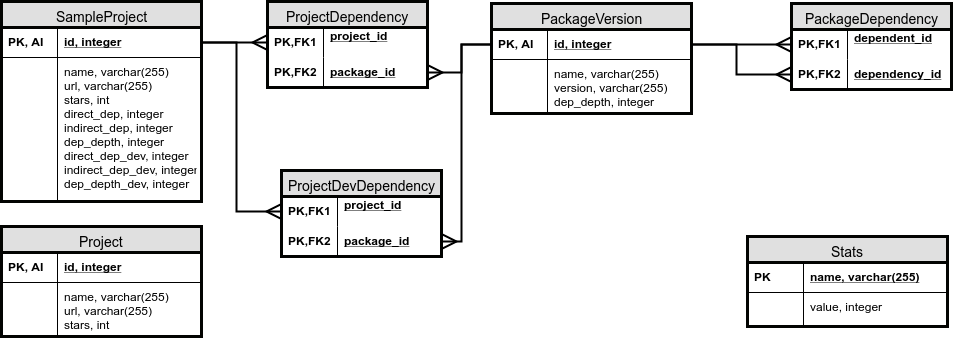
\includegraphics[scale=0.42]{npm_db}
  \caption{Databasen som har använts under undersökningen}
  \label{fig:dependency-db}
\end{figure}

Python-scriptet hämtade och lagrade information om Javascript-projekt med mer än 500 stjärnmarkeringar. En slumpmässig delmängd av dessa valdes därefter ut att ingå i undersökningen. För varje av dessa projekt utfördes sedan en analys av de beroenden som hittats i \texttt{package.json}. Antalet direkta beroenden lästes ut direkt ur \texttt{package.json}. För att undersöka indirekta beroenden användes en rekursiv metod som såg till npm-paketens vidare beroenden. Dessa undersöktes med hjälp av npm-kommandon på formen

\begin{center}
  \texttt{npm view \textit{paket}@\textit{version} dependencies \hyphen\hyphen json}.
\end{center}

Scriptet undersökte även det maximala djupet på dessa kedjor av paketberoenden från projekten. Då det även är av intresse att se hur beroenden påverkar utveckling skrevs scriptet så att det både undersöker \textit{dependencies} och \textit{devDependencies}. För en mer detaljerade beskrivning av programflödet se algoritm \ref{alg:analys} i bilaga \ref{app:algorithm}.

Då det till en början var okänt hur lång tid scriptet skulle behöva för att utföra undersökningen utfördes flera körningar med olika många utvalda projekt. Först valdes 1000 slumpmässiga paket som hade klassats som populära att ingå i undersökningen. Då scriptet kunde köras igenom under rimlig tid utfördes därefter en undersökning på samtliga projekt matchande popularitetskriteriet.

\subsection{Informationsinsamling}
För att få en mer robust förståelse för beroendens roll i Javascript utfördes en informationsinsamling av tidigare arbeten på området. Denna undersökning fokuserades på mer akademiska källor. Sökningar efter relevanta rapporter gjordes genom Google Scholar\footnote{\url{https://scholar.google.se/}} och Linköpings Universitetsbibliotek\footnote{\url{https://www.bibl.liu.se/}}.

Sökord som användes var bland annat ``Javascript'', ``npm'', ``dependencies'' och ``package''. Det var tydligt att ämnet för undersökningen var aktuellt då många av de arbeten som hittades var skrivna nyligen. Flera bra informationskällor hittades genom dessa sökningar. I dessa arbeten refererades även till andra relevanta källor som togs med i denna informationsinsamling.

\subsection{Projekterfarenheter}
I det utförda projektet har Javascript varit det huvudsakliga programmeringsspråket och npm har också använts för pakethantering. Det fanns redan i projektets kravspecifikation att vissa färdiga paket skulle användas. Detta inkluderade både stora ramverk som React och utvecklingsverktyg som ESLint.

Förutom en mängd beroenden som till en början krävdes för att påbörja arbetet tillkom flera under projektets gång. Detta inkluderade både \textit{dependencies} och \textit{devDependencies} i \texttt{package.json}. Under projektet uppkom flera öppna diskussioner om huruvida egna mjukvarukomponenter skulle implementeras eller färdiga paket användas. I dessa situationer övervägdes ofta kvalitet hos komponenterna samt till vilken grad de fyllde just det syfte som var nödvändigt. De främsta kvalitetsattributen som vägdes in var tillförlitlighet, effektivitet och hur enkelt paket kunde integreras. För att få en uppfattning om dessa egenskaper undersöktes artiklar och bloggar om andra utvecklares erfarenheter av att använda de paket som övervägdes. Paket som utvecklades aktivt och användes i många projekt antogs ofta vara av högre kvalitet. I vissa fall utfördes också test av att integrera färdiga komponenter i den existerande koden.

Då projektet består av flera separata applikationer finns i slutprodukten 3 separata kodbaser med varsin \texttt{package.json}-fil. Eftersom dessa filer har befunnit sig under versionshantering under hela projektet erbjuder de en logg över hur projektets beroenden har förändrats. Dessa ändringar tillsammans med de diskussioner och konsekvenser som har omgärdat dessa har givit upphov till en mängd erfarenheter för hur beroenden påverkat projektets utveckling och till viss del även slutproduktens kvalitet.

\section{Resultat}
\label{sec:joel_o-results}
Från de beskrivna metoderna har en mängd resultat sammanställts för att ge svar på frågeställningarna. Analysen av Javascript-projekt har givit en stor mängd kvantitativa resultat. Informationsundersökningen och projekterfarenheter erbjuder resultat av mer kvalitativ typ.

\subsection{Kvantitativa resultat}
\label{sec:joel_o-results-kvant}
Den 6 april 2018 passade 6~743 Javascript-projekt på Github in på tidigare nämnda definition av populära projekt. Av dessa innehöll 5~402, 80.1\% en \texttt{package.json} fil och ansågs därför vara av intresse för undersökningen. Samtliga data som presenteras här är baserade på dessa 5~402 projekt. Totalt hittades 114~249 beroenden varav 991, 0.87\% refererade till paket utanför npm-systemet.

De värden som är av intresse är projekts direkta beroenden, indirekta beroenden samt det maximala djupet på beroendekedjor. Medelvärde ($\bar{x}$), standardavvikelse ($\sigma$) och maxvärde ($x_{max}$) för dessa finns presenterade i tabell \ref{tab:beroende-data}. Minvärdet för samtliga är 0.

\begin{table}[H]
  \centering
  \begin{tabular}{c | c c c | c c c | c c c |}
    \cline{2-10}
    & \multicolumn{3}{c|}{Direkta Beroenden} & \multicolumn{3}{c|}{Indirekta Beroenden} & \multicolumn{3}{c|}{Beroendedjup} \\ \cline{2-10}
    & $\bar{x}$ & $\sigma$ & $x_{max}$ & $\bar{x}$ & $\sigma$ & $x_{max}$ & $\bar{x}$ & $\sigma$ & $x_{max}$ \\ \hline
    \multicolumn{1}{|c|}{\textit{dependencies}} & 6.76 & 12.5 & 153 & 95.02 & 200.21 & 1779 & 4.34 & 4.90 & 24 \\ \hline
    \multicolumn{1}{|c|}{\textit{devDependencies}} & 14.21 & 15.47 & 135 & 466.07 & 384.91 & 2202 & 10.42 & 5.71 & 21 \\
    \hline
  \end{tabular}
  \caption{Medelvärden, standardavvikelser och maxvärden för undersökta värden}
  \label{tab:beroende-data}
\end{table}

\begin{figure*}
    \centering
    \begin{subfigure}[]{0.5\textwidth}
        \centering
        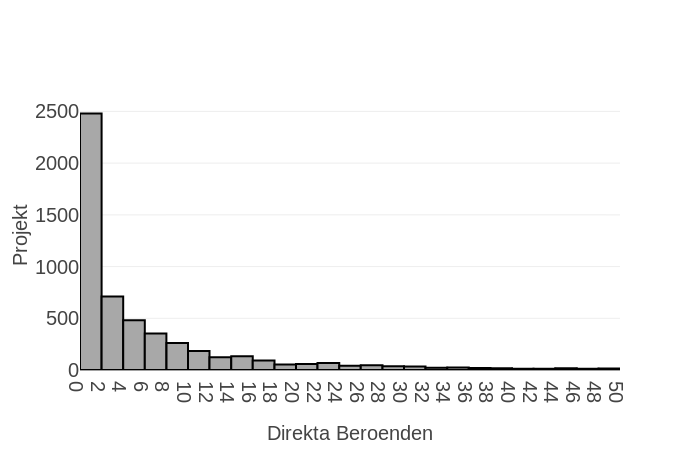
\includegraphics[height=5cm]{direct_dep}
        \caption{\textit{dependencies}}
    \end{subfigure}%
    ~
    \begin{subfigure}[]{0.5\textwidth}
        \centering
        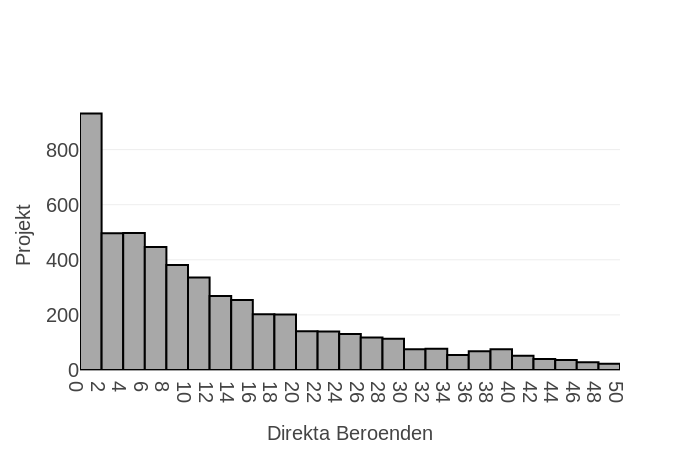
\includegraphics[height=5cm]{direct_dep_dev}
        \caption{\textit{devDependencies}}
    \end{subfigure}
    \caption{Histogram över projekt med maximalt 50 direkta beroenden}
    \label{fig:direct-dep}
\end{figure*}

Histogram över antalet beroenden presenteras i figur \ref{fig:direct-dep}. Av de analyserade projekten hade 1853, 27.50\% inga beroenden. Samma siffra för \textit{devDependencies} är betydligt lägre på endast 696 projekt, 12.90\% med inga beroenden för utveckling. Från histogrammen syns det tydligt att den största gruppen av projekt har inga eller endast några få beroenden. För \textit{dependencies} avtar mängden projekt hastigt för större antal beroenden. \textit{DevDependencies} visar inte en lika snabb nedgång för större antal beroenden.

\begin{figure*}
    \centering
    \begin{subfigure}[]{0.5\textwidth}
        \centering
        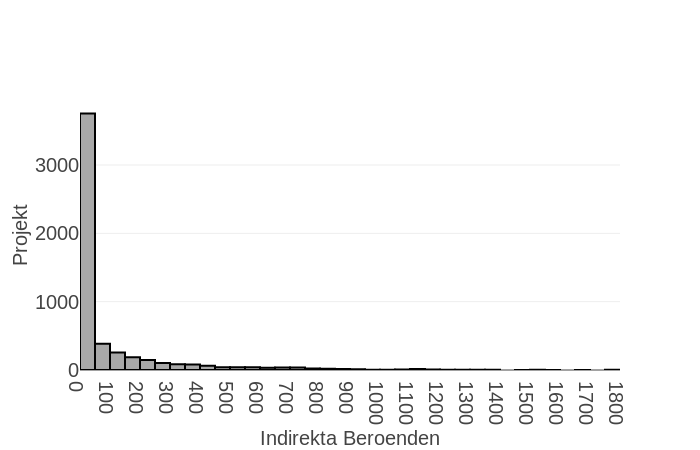
\includegraphics[height=5cm]{indirect_dep}
        \caption{\textit{dependencies}}
    \end{subfigure}%
    ~
    \begin{subfigure}[]{0.5\textwidth}
        \centering
        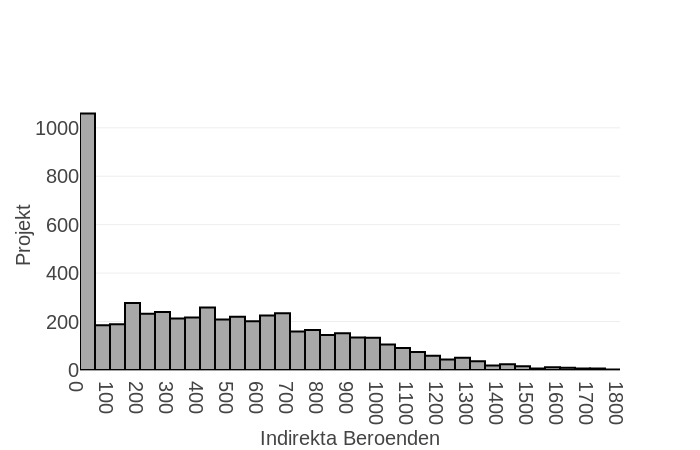
\includegraphics[height=5cm]{indirect_dep_dev}
        \caption{\textit{devDependencies}}
    \end{subfigure}
    \caption{Histogram över projekt med maximalt 1800 indirekta beroenden}
    \label{fig:indirect-dep}
\end{figure*}

En liknande fördelning över \textit{dependencies} syns för indirekta beroenden i figur \ref{fig:indirect-dep}. Här är dock antalet \textit{devDependencies} mycket utspritt. Förutom den stora mängd med inga eller några få indirekta beroenden finns en något jämn fördelning mellan 100-700 beroenden. Detta betyder att det finns en substantiell mängd projekt med flera hundra indirekta beroenden för utveckling.

\begin{figure*}
    \centering
    \begin{subfigure}[]{0.5\textwidth}
        \centering
        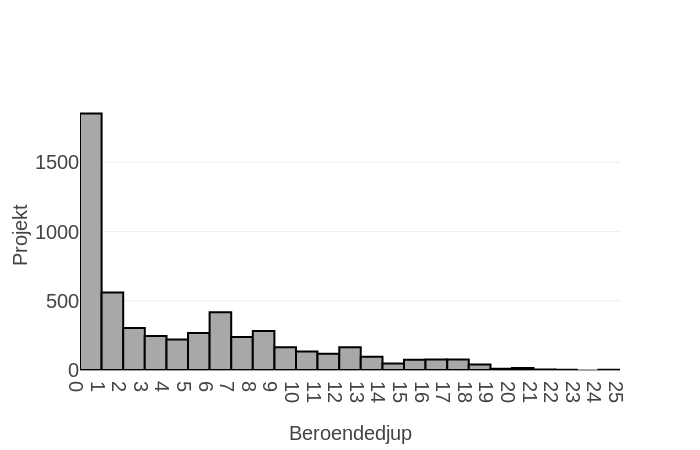
\includegraphics[height=5cm]{dep_depth}
        \caption{\textit{dependencies}}
        \label{fig:dep-depth-dependencies}
    \end{subfigure}%
    ~
    \begin{subfigure}[]{0.5\textwidth}
        \centering
        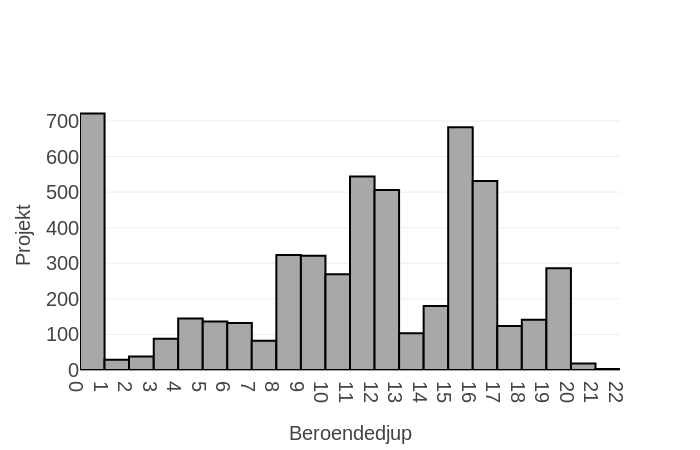
\includegraphics[height=5cm]{dep_depth_dev}
        \caption{\textit{devDependencies}}
        \label{fig:dep-depth-devDependencies}
      \end{subfigure}
    \caption{Histogram över projektens beroendedjup}
    \label{fig:dep-depth}
\end{figure*}

Också djupet av beroenden är mycket större för \textit{devDependencies}, även om det maximala djupet av 24 i tabell \ref{tab:beroende-data} är för \textit{dependencies}. I histogrammet \ref{fig:dep-depth-dependencies} syns en liknande fördelning av djup som för antal beroenden. En dominerande del av projekten saknar beroenden, här dock med en något jämn fördelning av projekt med 2 till 9 nivåer. För \textit{devDependencies} syns dock en spretig uppdelning i figur \ref{fig:dep-depth-devDependencies}. Även om många projekt har 0 beroendenivåer finns här nästan lika stora mängder runt djup 12 och 16. Det är tydligt att det är mycket vanligt att Javascript-projekt har \textit{devDependencies} som sträcker sig många nivåer genom npm-systemet.

\subsection{Påverkan på utvecklingsprocessen}

Färdiga paket har under det genomförda projektet erbjudit många möjligheter. Det stora ramverket React har varit centrala för utvecklingen av användargränssnitt och interaktion. Speldelen av projektet har kunnat förenklats genom användandet av paketet PixiJS. Flera paket har även varit centrala för utvecklingsarbetet. Speciellt paket för testning har erbjudit automatisering som inte hade varit möjlig utan dessa. Det är ej troligt att kodens kvalitet till samma grad hade kunnat garanterats genom projektet utan dessa verktyg.

Att arbeta med färdiga paket tycks även till viss del förändra vad som krävs av utvecklare. När paket adderades till projektet var det viktigaste att dessa integrerades korrekt. Detta krävde kunskap om paketen som användes och om hur de skulle passa in i systemet som utvecklades. Här spelar utvecklarens tidigare vana av paketen samt dokumentation en stor roll. Detta är till viss del skilt från egenskaper som logiskt tänkande och algoritmisk problemlösning som annars associeras med mjukvaruutveckling.

Att i utvecklingsarbete integrera flera färdiga paket har visat sig även skapa en något ökad osäkerhet i felsökning. Det har i det genomförda projektet uppkommit situationer då det inte är klart om buggar beror på den egna koden, kod i importerade paket eller en felaktig integration av paket. Dessa ovissheter ökar med ovetskapen om paketen som arbetas med.

Datan från undersökningen av Javascript-projekt visar att hjälppaket för utvecklingsarbetet används i stor utsträckning. Dessa paket har ofta flera beroenden under sig, vilket leder till ett utvecklingsarbete som vilar på att stora mängder paket fungerar korrekt. S. Scott Henry har studerat en problematisk förändring till paketet \textit{mkdirp} som ofta användes i utvecklingsprocesser.\cite{Henry2017} Denna förändring skapade stora problem för utvecklare som använde den nya versionen, men problemen åtgärdades mycket snabbt. Exemplet visar på hur paket som är centrala för utvecklares arbete är kritiska för utvecklingsprocessen, men också att problem som direkt når utvecklare löses mycket effektivt.

\subsection{Påverkan på säkerhet och tillförlitlighet}
Inkludering av färdiga paket ökar mängden kod i projekt och därmed möjliga problem med säkerhet och tillförlitlighet. Att paket oftast är publicerade som open-source och används i många olika projekt är dock anledningar att tro att denna kod har en hög kvalitet.\cite{coverity-scan2013}

Det finns trots detta flera exempel där säkerhetsproblem har förekommit i npm-paket och genom beroenden påverkat andra paket och projekt. Joseph Hejderup utförde 2015 en undersökning av dessa problem.\cite{Hejderup2017} De vanligaste problemen i npm-paket har visat sig vara känslighet för attacker som \textit{cross site scripting} och \textit{denial of service} (då Javascript används som server-språk). Hejderup identifierade i sin undersökning över 1~500 paket med beroenden till paket med säkerhetsproblem. En grov uppskattning gav att ungefär 1\% av npm-ekosystemet kunde vara i riskzonen för kända säkerhetsproblem.

I tidigare nämnda arbete poängteras också att utvecklare till paket ofta inte visat någon medvetenhet över säkerhetsproblem i beroenden. Detta beror möjligen på att många paket är utdaterade och inte längre underhålls kontinuerligt. Denna observation visar på vikten för utvecklare att ha en stor medvetenhet om hur pass uppdaterade integrerade paket är. För att kunna garantera säkerhet i Javascript är det troligen nödvändigt att till viss del vara insatt i problem och underhåll för de paket som beroenden finns till.

En större kodmängd av jämn kvalitet leder till större chans för buggar och en lägre tillförlitlighet. Vid inkludering av färdiga paket kan dock kod förväntas hålla en hög kvalitet. Erfarenheter från det gångna projektet visar att introducerade problem mycket sällan kommer från buggar i de integrerade paketen. Ofta kommer problemen istället från felaktig integration och användning av paketen.

I de fall fel uppstår på grund av inkludering av färdiga paket (antingen direkt i paketen eller i integrationen) påverkas även systems tillförlitlighet av mängden resurser som finns för reparation av mjukvaran. God dokumentation och större mängder utvecklare med kunskap av arbete med vissa paket gör att problem kan förväntas lösas enklare jämfört med egenproducerad kod. Detta förkortar MTTR och minskar den tid system kan förväntas vara otillgängliga.

\section{Diskussion}
\label{sec:joel_o-discussion}
Detta arbete bör ge en viss insikt i tillståndet för Javascript och npm-ekosystemet. Det erbjuder en ytlig, kvantitativ insikt i beroenden, men ger inga svar på varför utvecklingen har lett till dessa sammankopplingar av mjukvaruprojekt. Här finns definitivt plats för en analys som täcker både teknisk implementation, sociala interaktioner i utvecklargemenskaper och affärsmässiga beslut. Eftersom trender visar att beroenden till färdiga paket i Javascript ökar\cite{Wittern:2016} och liknande ekosystem som npm existerar även för andra programmeringsspråk kommer en ökad förståelse för denna utveckling troligen vara av intresse i framtiden.

Något värt att fundera kring är naturen av populära Javascript-projekt. Det är mycket tänkbart att de flesta av dessa är projekt som i sig består av paket för utvecklare att använda. I många fall är projekten antagligen även npm-paket. Det kan finnas ett värde i att göra en skillnad på olika kategorier av Javascript-projekt. En uppdelning i exempelvis paket, färdiga webbapplikationer och server-applikationer skulle kunna erbjuda intressanta resultat. Det finns dock svårigheter i att göra den uppdelningen så att en kvantitativ analys av samma typ som i detta arbete kan utföras. Kategoriseringen skulle troligen behöva förlita sig på metadata så som beskrivningstexter för projekt.

\subsection{Metod}
\label{subsec:joel_o-discussion-method}
Den metod som har använts för analys av Javascript-projekt anses ge en till stor del korrekt bild av den undersökta datamängden. Då den rena datan tillhandahålls från Github och npm är korrektheten hos denna direkt beroende till att dessa tjänster erbjuder rätt information. Vissa felaktigheter kan dock ha uppstått av förändringar i projekt eller paket under den tid analysen har utförts. Då den fullständiga undersökningen tagit en längre tid kan datan inte sägas representera ett tillstånd vid en specifik tidpunkt. Dessa felaktigheter anses dock vara mycket små i förhållande till storleken på den datamängd som har analyserats.

En stor del av beroendens konsekvenser på utvecklingsprocessen beskrivs baserat på erfarenheter från det utförda projektet. Det finns i detta en viss risk att resultaten blir begränsade till att endast beskriva påverkan på utvecklingsarbete i liknande projekt. Exempelvis har projektets paketanvändning till viss del kretsat kring React och npm-paket som fungerar bra med detta ramverk. Att avgöra till vilken grad erfarenheterna av pakethantering är projektspecifika är komplext. Troligen ger en stor del av de mer generella erfarenheterna en givande bild av påverkan på utvecklingsprocessen. Mer specifika erfarenheter av enskilda paket har dock undvikits då dess värde för att svara på frågeställningarna är högst osäkert.

De källor som har använts i detta arbete är till stor del av akademisk natur i form av rapporter, examensarbeten och böcker. Detta är ett aktivt val, som har tagits med förhoppningen att dessa ska hålla en hög kvalitet och trovärdighet. Examensarbeten hålls möjligen inte till samma standard som publicerade akademiska rapporter, men de som har använts anses vara trovärdiga. För en bedömning av källors trovärdighet har författares tidigare och fortsatta arbete undersökts ytligt. Examensarbeten har till viss del även bedömts baserat på handledares arbete och intressen.

\subsection{Resultat}
\label{subsec:tim-discussion-results}
Resultaten från detta arbete pekar på att mjukvaruutveckling i Javascript baserad runt färdiga paket är en etablerad metod och inget tyder på att denna utveckling avtar. Dessa arbetssätt påverkar definitivt utvecklingsprocesser och den mjukvara som levereras idag. Om detta dras till sin spets är det tänkbart att programmerarens roll kan få vissa förändringar i framtiden.

En förhoppning är att resultaten ska erbjuda viss vägledning för arbete med beroenden i Javascript-projekt. Det ger troligen en god introduktion till hur beroenden hanteras i npm-ekosystemet. Resultaten för frågeställning \ref{joel_o-fs:2} ger någon insikt av vad som kan förväntas i ett projekt med beroenden till färdiga paket. Förhoppningar finns också att resultaten från frågeställning \ref{joel_o-fs:3} ska erbjuda vissa riktlinjer för hur arbete med beroenden bör bedrivas för att maximera säkerhet och tillförlitlighet.

Resultaten från den genomförda undersökningen visar på en skillnad mellan beroenden i form av \textit{dependencies} och \textit{devDependencies}, men ger ingen tydlig förklaring till denna. En vidare analys av detta skulle kunna göras baserat på fallstudier. Baserat på det utförda projektet är det troligt att det höga antalet \textit{devDependencies} har att göra med grupper av utvecklingsverktyg som mycket ofta används tillsammans. En undersökning som grupperar paket på detta sätt skulle kunna erbjuda en bra bild över npm-ekosystemet.

Undersökningen som har utförts berör endast open-source Javascript-projekt. Arbetet bör därför endast anses ge en bild av denna sorts projekt. Det är tänkbart att proprietära projekt besitter andra egenskaper än vad som presenteras här. Resultat för frågeställning \ref{joel_o-fs:2} och \ref{joel_o-fs:3} påverkas dock troligen inte av detta.

\section{Slutsatser}
\label{sec:joel_o-conclusion}
De presenterade resultaten ger tydliga svar på frågeställning \ref{joel_o-fs:1}. Frågeställning \ref{joel_o-fs:2} och \ref{joel_o-fs:3} är något mer öppna och inget resultat kan rimligen ge ett fullständig svar. De resultat som presenterats ger dock en kvalificerad insikt i hur beroenden till färdiga paket påverkar mjukvara.

\subsection*{\ref{joel_o-fs:1} Hur många beroenden till färdiga paket finns i populära open-source Javascript-projekt?}

En undersökning av open-source Javascript-projekt på GitHub med minst 500 stjärnmarkeringar har genomförts. Data om direkta beroenden, indirekta beroenden och beroendedjup har tagits fram och presenteras till fullo i stycke \ref{sec:joel_o-results-kvant}. Dessa Javascript-projekt har i genomsnitt 6.76 direkta beroenden och 95.02 indirekta beroenden. Samma värden för beroenden som krävs för utvecklingsarbete på projekten är 14.21 respektive 466.07. I allmänhet har projekten mycket fler beroenden av typen \textit{devDependencies} än \textit{dependencies}.

\subsection*{\ref{joel_o-fs:2} Hur påverkar beroenden till färdiga paket utvecklingsprocessen för Javascript-projekt?}

Färdiga paket underlättar på många sätt utvecklingsarbetet då komponenter som annars hade behövts byggas från grunden kan importeras in i projekt. Dessa paket kan bland annat vara ramverk för hela system som utvecklaren behöver förhålla sig till. Färdiga paket kan även erbjuda verktyg för att underlätta själva utvecklingsprocessen, men inte direkt påverka slutprodukten. Arbete med färdiga paket ställer till viss del speciella krav på utvecklare. Det har visat sig viktigt att utvecklare kan integrera paketen korrekt i systemet.

\subsection*{\ref{joel_o-fs:3} Hur påverkar beroenden till färdiga paket säkerhet och tillförlitlighet för mjukvara skriven i javascript?}

Genom beroenden kan säkerhetsproblem i ett paket spridas till flera Javascript-projekt och paket. Om projekt förlitar sig på paket som inte aktivt underhålls finns risker att denna sorts säkerhetsproblem förblir okorrigerade. Det tycks vara viktigt att utvecklare har en viss insikt i säkerhet och underhåll för de paket som projekt har beroenden till.

Färdiga pakets påverkan på tillförlitlighet beror till stor del på hur utvecklare integrerar paketen i projekt. Det finns anledningar att förvänta sig att kod i färdiga paket håller en hög kvalitet. Buggar kan dock introduceras om utvecklare på grund av okunskap använder paket felaktigt. Vid fel kan informationsresurser om olika paket underlätta reparation av mjukvarukomponenter och därmed sänka MTTR.

\section{Algoritm för analys av projektberoenden}
\label{app:algorithm}

Algoritm \ref{alg:analys} användes för den analys av Javascript-paket som beskrivs i \ref{subsec:joel_o-method-analys}.

\begin{breakablealgorithm}
\caption{Javascript Project Analysis} \label{alg:analys}
\begin{algorithmic}[1]
  \Function{AnalysePackage}{$package$}
    \If{\Call{InDatabase}{$package$}}
      \State \Return
    \EndIf
    \State
    \State $pkgDeps \gets$ \Call{GetNpmDependencies}{$package$}
    \State \Call{SavePackageDependencies}{$pkgDeps$}
    \State
    \ForAll{$package \in pkgDps$}
      \State \Call{AnalysePackage}{$package$}
    \EndFor
  \EndFunction
  \State
  \Function{AnalyseProjects}{}
    \State $projects \gets $ \Call{GetGitHubProjects}{ }
    \State $sampleProjects \gets n$ random entries from $projects$
    \State
    \State $nonNpmC \gets 0$
    \ForAll {$project \in sampleProjects$}
      \If{\Call{HasPackageJson}{$project$}}
        \State $packageInfo \gets $ \Call{GetPackageJson}{$project$}
        \State $deps \gets $ \textit{dependencies} in $packageInfo$
        \State $devDeps \gets $ \textit{devDependencies} in $packageInfo$
        \State
        \State \Call{SaveProjectDependencies}{$project, deps, devDeps$}
        \State
        \State $directDependencies \gets |deps|$
        \State $directDevDependencies \gets |devDeps|$
        \State
        \If {$directDependencies > 0$}
          \ForAll {$package \in deps$}
            \State\Call{AnalysePackage}{$package$}
          \EndFor
          \State
          \State $depth \gets$ \Call{MaxDepth}{$deps$} $+ 1$
        \Else
          \State $depth \gets 0$
        \EndIf
        \State
        \If{$directDevDependencies > 0$}
          \ForAll {$package \in devDeps$}
            \State \Call{AnalysePackage}{$package$}
          \EndFor
          \State
          \State $devDepth \gets$ \Call{MaxDepth}{$devDeps$} $+ 1$
        \Else
          \State $DevDepth \gets 0$
        \EndIf
        \State
        \State $indirectDependencies \gets$ \Call{countPackages}{$deps$}
        \State $indirectDevDependencies \gets$ \Call{countPackages}{$devDeps$}
        \State \Call{SaveProjectData}{$project, directDependencies, directDevDependencies, depth,$\par
        \hskip\algorithmicindent\hskip\algorithmicindent\hskip\algorithmicindent $devDepth, indirectDependencies, indirectDevDependencies$}
      \Else
        \State $nonNpmC \gets nonNpmC + 1$
      \EndIf
    \EndFor
  \EndFunction
\end{algorithmic}
\end{breakablealgorithm}

Nedan följer förtydliganden av de funktioner som används i algoritm \ref{alg:analys}.

\begin{labeling}{\textbf{SavePackageDependencies}}
  \item [\textbf{InDatabase}] Kontrollera om information om ett paket finns sparad i databasen
  \item [\textbf{GetNpmDependencies}] Hämta beroenden (i detta fall endast \textit{dependencies}) för ett paket från npm
  \item [\textbf{SavePackageDependencies}] Spara ett pakets beroenden i databasen
  \item [\textbf{GetGitHubProjects}] Hämta data för projekt klassade som populära från GitHub
  \item [\textbf{HasPackageJson}] Kontrollera om ett projekt innehåller filen \texttt{package.json} och därmed använder sig av npm som pakethanteringssystem
  \item [\textbf{GetPackageJson}] Hämta data från filen \texttt{package.json} för projektet på GitHub
  \item [\textbf{SaveProjectDependencies}] Spara beroenden från projektet i databasen
  \item [\textbf{MaxDepth}] Hitta det maximala djupet av beroenden från något av de givna paketen
  \item [\textbf{CountPackages}] Räkna antalet paket som genom beroendereferenser kan nås från de givna paketen
  \item [\textbf{SaveProjectData}] Spara kvantitativ information om ett pakets beroenden i databasen
\end{labeling}


\chapter{Undersökning av typning i Javascript av Alexander Wilkens}

\section{Introduktion}
\label{sec:alexander-introduction}
Inom programmering finns en konstant debatt kring olika sorters typning i programmeringsspråk. Det finns dynamiskt typade språk, som till exempel Javascript eller Python, men också strikt typade språk, som Java eller Typescript. Utvecklingsarbetet i de olika språken skiljer sig åt just på grund av den olika typningen, men trots det överlappar deras användningsområden väldigt ofta. Vad är de olika för- och nackdelarna av att använda ett dynamiskt typat språk som Javascript istället för ett strikt typat?

\subsection{Syfte}
\label{subsec:motivation}

Syftet med denna undersökning är att få en bättre bild över hur Javascripts dynamiska typning påverkar utveckling i språket, men också hur språket ställer sig mot alternativ med striktare typning. Arbetet kommer förhoppningsvis ge insikt i varför man skulle välja Javascript över alternativen som finns, eller tvärt om.

\subsection{Frågeställning}
\label{subsec:research-questions}

\begin{enumerate}
\item\label{alexander-fs:1} Hur påverkades utvecklingsarbetet av Javascripts typsystem?

\item\label{alexander-fs:2} Hur påverkades slutprodukten av Javascripts typsystem?

\item\label{alexander-fs:3} När vill man använda ett strikt typat språk istället för Javascript?

\end{enumerate}


\subsection{Avgränsningar}
\label{subsec:delimitations}

Undersökningen kommer fokusera på kvantitativ data från projekt vars primära utvecklingsspråk är Javascript, Javacript med Flow eller Typescript, vilka beskrivs i mer detalj senare under \ref{sec:alexander-theory}. Undersökningen kommer inte innefatta andra dynamiska och strikt typade språk, som Java eller Python, dock kan dessa förekomma i de källor som refereras.

%\nocite{scigen}
%We have included Paper \ref{art:scigen}

%%%%%%%%%%%%%%%%%%%%%%%%%%%%%%%%%%%%%%%%%%%%%%%%%%%%%%%%%%%%%%%%%%%%%%
%%% Intro.tex ends here


%%% Local Variables: 
%%% mode: latex
%%% TeX-master: "demothesis"
%%% End: 

\section{Bakgrund}
\label{sec:alexander-background}

Javascript är idag ett mycket populärt programmeringsspråk som kan köras på en stor majoritet av alla enheter som har tillgång till en webbläsare. Språket har fått en hel del kritik genom åren, där mycket av kritiken fokuserat på språkets sätt att hantera odefinierade variabler, samt hur Javascript generellt är ganska dåligt på att meddela när någonting kan ha gått fel.

Debatten kring för- och nackdelarna med dynamiskt och strikt typade språk är en som varit vid liv länge \cite{old-type-debate}. Denna debatt har förstås följt med då Javascript, ett dynamiskt typat språk, blev det språk som dominerar programmering av webbsidor och webbapplikationer. På senare år har dock alternativ som Flow och Typescript, som beskrivs mer under \ref{sec:alexander-theory}, blivit mer och mer populära. Dessa introducerar strikt typade alternativ till Javascript.

\subsection{Projekterfarenheter}
I projektet som denna rapport tillhör har projektgruppen nästan exklusivt använt sig av Javascript. Detta berodde på projektmedlemmarnas tidigare erfarenheter med språket tillsammans med rekommendationer och önskemål från kunden. Rekommendationerna från kunden var baserade på deras egna erfarenheter med språket och det faktum att majoriteten av deras kodbas var skriven i det. Kunden uttryckte också att användningen av Typescript kunde ses som onödig.
\section{Teori}
\label{sec:alexander-theory}

Detta kapitel beskriver den teori som krävs för att förstå den metod och resultat som presenteras.

\subsection{Typer i Javascript}

Analysen för detta arbete baseras på hur olika typning i språket påverkar koden som skrivs. Det är därför viktigt att ha en tydlig förståelse för vilka typer som finns i Javascript och hur de hanteras. Javascript är ett dynamiskt typat språk vilket i praktiken innebär att utvecklaren inte specificerar vilken typ en variabel har, utan detta bestäms istället vid körtid beroende på vad variabeln blir tilldelad för värde. Motsatsen till detta är statisk typning, då till exempel en kompilator verifierar typen av variabler innan koden körs.

Javascript har totalt sex primitiva datatyper: \textit{String}, \textit{Number}, \textit{Boolean}, och \textit{Symbol}, \textit{null} och \textit{undefined}.\cite{javascript-primitives}

\subsection{Påtvingade typer}

Från sin design som ett dynamiskt typat språk följer att Javascript är väldigt uttrycksfullt.\cite{javascript-type-coersion} Med detta menas att språket väljer att tolka en hel del saker själv istället för att låta användaren specificera det explicit. Detta hänger ihop med Javascripts sätt tvinga typer. Ett snabbt exempel visar hur Javascript själv väljer att konvertera värden beroende på vilken operator som används:

\begin{lstlisting}[language=JavaScript]
var a = 1; // Number
var b = "1"; // String
var c = a + b; // "11"
var c = a - b; // 0
\end{lstlisting}




På översta raden bestämmer sig språket för att använda ``+'' som konkatenering istället för summation och konverterar därför variabeln \texttt{a} till en sträng och lägger sedan ihop \texttt{a} och \texttt{b}. I det andra exempel fungerar ``-'' endast som subtraktion så det enda logiska blir att konvertera b till ett nummer och sedan utföra operationen. Eftersom Javascript inte har något inbyggt sätt att specificera vilken typ en variabel ska ha kan exempel som detta ofta förekomma under utveckling.

Denna typ av uttrycksfullhet ger utvecklare möjlighet att snabbt utveckla applikationer utan att behöva låsa sig till vilken typ variabler och i sin tur olika delar av koden har.


\subsection{Introduktion av Flow och Typescript}

Eventuella problem med påtvingade typer som beskrivs ovan är något som är väldebatterat när det kommer till Javascript. Många anser att språket fungerar utmärkt som det är och utvecklar storskaliga projekt med det. Andra är dock inte lika nöjda med det och flera stora mjukvaruföretag har utvecklat egna verktyg för att lösa de eventuella problem de har med språket.\cite{js-bad} Två av dessa är Facebook och Microsoft som har utvecklat Flow \cite{info-flow} respektive Typescript \cite{typescript}.

\subsubsection{Flow}

Flow är ett verktyg som används för att komplettera Javascript. Det ger utvecklare möjligheten att explicit specificera vilken typ en variabel är eller vad en funktion returnerar. Facebook marknadsför dock att med Flow ska utvecklaren inte behöva explicit specificera vilken typ en variabel behöver vara. Istället ska verktyget vara smart nog att bestämma vilken typ variabeln är och fortfarande markera om eventuella konflikter uppstår. Flow gör också en extra kontroll på nyckelordet \texttt{this} som förekommer ofta i Javascript-utveckling. Ett vanligt problem utvecklare stöter på är att de försöker använda nyckelordet för att hänvisa till den delen av koden där funktionen ligger, men när funktionen som använder nyckelordet anropas så refererar \texttt{this} till något annat. Detta sker vanligtvis i en callback-funktion, alltså en funktion som anropas när en annan funktion är klar, och kan leda till en del frustration om man inte är försiktig. Det som Flow tillför är att verifiera vilken funktion som använder sig av nyckelordet redan vid kompilering och kan alltså bestämma om det kommer orsaka problem vid körtid eller inte. 

\subsubsection{Typescript}

Till skillnad mot Flow så är Typescript inte bara ett verktyg som kan användas i projekt, utan ett helt programmeringsspråk som kompileras till Javascript innan körning. Typescript erbjuder, precis som Flow, en möjlighet för utvecklare att explicit specificera vilken typ en variabel är. Dock erbjuder språket en hel del andra funktioner, som mer utvecklade klasser och gränssnitt, tillsammans med andra funktioner som inte är speciellt intressanta för detta arbete.
Någonting som både Flow och senare versioner av Typescript har gemensamt är hur variabler som antingen är \textit{null} eller \textit{undefined} hanteras. I vanlig Javascript ges generellt ingen feedback om man försöker göra operationer med variabler som är odefinierade, vilket kan anses som en svaghet i språket. I både Flow och Typescript kan man däremot få kompilatorn att ge ett fel vid sådana operationer, om inte utvecklaren explicit specificerar att dessa är okej.


\section{Metod}
\label{sec:alexander-method}

För att försöka svara på frågeställningarna har information från tidigare publicerade källor och undersökningar analyserats och sammanställts. Information från tidigare forskning har också kompletterats med erfarenheter från det projekt som gruppen utfört. 

\subsection{Information från tidigare forskning}

Då de erfarenheter gruppen upplevt inom detta område under projektets gång har varit begränsade så har ytterligare forskning och undersökningar om fler och större projekt använts. Mycket av forskning har hittats med hjälp av sökfunktioner på Google Scholar och biblioteket vid Linköpings universitet. De primära söktermerna som användes var en blandning av \textit{Javascript}, \textit{Typescript} och \textit{typing} vilket gav en stor mängd resultat. Urvalet av resultat som källa till denna rapport gjordes genom att läsa eventuella sammanfattningar till relevanta sökresultat. Resultaten som innehöll direkta undersökningar mellan Javascript och Typescript ansågs vara mest relevanta och undersöktes sedan vidare. Trots det undersöktes även vissa resultat som inte hade denna direkta undersökning i hopp om att ge en bredare kunskapsgrund till denna rapports undersökning. Den kvantitativa data som presenteras kommer främst från publicerade konferenshandlingar.

\subsection{Projektgruppens erfarenheter}
Trots att de erfarenheter som gruppen upplevt under projektets gång varit begränsade har det ändå varit viktigt att fånga på grund av deras direkta påverkan på den produkt som utvecklats. För att få med personliga erfarenheter har projektgruppen frågats i efterhand hur de kände att typsystemet som finns i Javascript har påverkat deras utvecklingsprocess och produkten. Frågorna kring detta ställdes något informellt i gruppens Slack, där de som kände att de hade unika erfarenheter besvarade frågan. Eventuella buggar och andra problem som orsakats av typsystemet ligger också till viss del kvar i versionshanteringssystemet som gruppen använder. Utöver dessa mer direkta metoder har också generella återkommande problem och frågor kring typsystemet noterats.

\subsection{Kritik av källor}
För att resultat som presenteras ska anses vara trovärdigt och tillförlitligt kommer viss kritik av källor och egna undersökningar föras fram. Denna finns under kapitel \ref{sec:alexander-discussion}. Kritiken kommer innefatta validiteten hos de källor och undersökningar som använts, tillsammans med en presentation av för- och nackdelar av resultatet från gruppens erfarenheter. 
\section{Resultat}
\label{sec:alexander-results}

Under denna rubrik framförs de resultat som samtliga undersökningar producerat. Resultaten omfattar hur buggar kan hanteras av typsystem, hur ett typsystem hjälper utvecklingsmiljöer och utvecklare samt projektgruppens resultat med typsystemet som finns i Javascript. Dessa resultat diskuteras vidare i nästkommande kapitel.

\subsection{Detektion av buggar i olika typsystem}
För att kommentera på detektionen av buggar i olika typsystem presenteras resultat från \cite{type-or-not-proceed}. Gao et al. undersöker flera stora open-source-projekt skrivna i Javascript.  Undersökning går ut på att bestämma en undre approximation på hur stor del av historiska buggar kunde ha detekterats genom att introducera ett strikt typsystem. Typsystemen som använts i undersökningen är Flow och Typescript som beskrevs tidigare under \ref{sec:alexander-theory}. En fullständig beskrivning av metoden kan ses här\cite{type-case-study}. Metoden går kort sagt ut på att hitta en buggfix, plocka ut den ändrade delen av koden innan den blev ändrad och introducera explicita typer där det är möjligt. När detta är gjort analyseras koden av respektive kompilator där författarna kollar om typsystemet ger en indikation att något fel. Undersökningen innefattade endast publika buggar, alltså buggar som blivit introducerade i projektets versionshaneringsystem. Resultaten av undersökningen visar att båda typsystemen lyckades hitta 15\% av de undersökta buggarna. 

\subsection{Integration i utvecklingsmiljö och kodkomplettering}
Resultaten för denna del kommer från \cite{Fischer:2015:EIE:2816707.2816720}. Fischer et al. undersöker hur typsystemet i ett språk påverkar utvecklingsmiljöns möjligheter att visa hjälpsam information till användaren. De undersökte specifikt skillnaden mellan Javascript och Typescript i utvecklingsmiljön MS Visual Studio. I undersökningen fick deltagarna försöka sätta sig in en redan existerande kodbas, skriven i både Javascript och Typescript, och försöka implementera en viss funktionalitet. Den fullständiga metoden för undersökningen finns tillgänglig i referensen. Undersökningen innefattade Javascript och Typescript, både med och utan kodkomplettering igång. Resultaten visar på att utvecklingsarbetet gjort i Typescript var betydligt mycket snabbare i alla fall som testats. Skillnaderna med kodkomplettering visade resultat som var betydligt mer varierande. Trots det anser författaren att kodkomplettering ger en något marginell förbättring i utvecklingstid.

\subsection{Projektgruppens resultat}

Under projektets gång har gruppen stött på en hel del buggar som orsakats av Javascripts typsystem. Majoriteten av dessa buggar berodde på bristande indikation att variabler var odefinierade, då många operationer fungerar utan problem ändå. Ett specifikt exempel med en förklaring kan ses i figur \ref{fig:buggy-code-explained}. Denna kod skulle se till att kontrollapplikationen skickade information till servern med ett visst tidsintervall. Eftersom den använda variabeln inte var definierad ledde detta till en svårhittad bugg och en något misslyckad demo då systemet blev överbelastat eftersom för mycket data skickades.

\begin{figure*}[h]
    \begin{lstlisting}[language=JavaScript]
        var sendTime = 1000/this.options.tickrate; // this.options.tickrate was undefined -> sendTime === NaN
        setInterval(this.tick, sendTime); // this.tick is called as often as possible
    \end{lstlisting}
    \caption{Kod som orsakat problem}
    \label{fig:buggy-code-explained}
\end{figure*}

\section{Diskussion}
\label{sec:alexander-discussion}

I detta kapitel kommer både metoden och resultatet som tagits upp innan att diskuteras. Eftersom ingen egen kvantitativ undersökning gjorts, förutom de erfarenheter gruppen stött på, kommer metoden och resultatet från forskningen som använts också analyseras och värderas.  Något värt att nämna om båda de undersökningarna som studerats är att båda baserats på existerande kodbaser. Det är alltså svårt att dra slutsatser kring utveckling av nya projekt, precis som det gruppen utfört. Frågeställningen är dock något baserad på generellt utvecklingsarbete inom projekt med Javascript, vilket betyder att nystartade projekt inte nödvändigtvis är lika relevanta. Något som framkommer i både [ref1] och [ref2] är att författarna menar att nyttan av ett typat system ökar med projektets storlek. 


\subsection{Metod}
\label{subsec:alexander-discussion-method}

Metoden för att presentera resultaten till denna rapport har främst bestått av att sammanställa information från tidigare publicerad forskning. Som det nämndes i början av metoden påbörjades en egen undersökning kring stora open-source-projekt på Github. Tanken bakom denna undersökning var att försöka bestämma kvaliteten av ett projekt på ett kvantitativt sätt och jämföra Javascript och Typescript. Ett beslut om att inte fortsätta med undersökning togs dock när ingen rimlig storhet för kvalitet av projekt kunde bestämmas.

Generellt tycker jag att metoden med att basera resultaten på tidigare forskning fungerade väldigt bra. För det första var det väldigt enkelt att hitta relevanta publicering via bibliotekets hemsida och Google Scholar. Jag lyckades hitta texter som var mycket välskrivna och hade en riklig mängd med källor att vidare studera.

Metoden för att fånga gruppens egna erfarenheter kring typning i Javascript kan absolut förbättras. För denna undersökning blev det mer en informell insamling av erfarenheter under projektets gång, och en mer formell avslutande fråga. För att förbättra insamling borde grupp tillfrågats att notera varje gång de stötte på någon märkvärdigt med typsystemet. Detta hade lett till fler användbara exempel att redovisa i resultatet.

\subsection{Resultat}
\label{subsec:alexander-discussion-results}

Resultaten som presenterades från de kvantitativa undersökningarna ger en mycket tydlig bild hur Javascript står mot sina typade alternativ. Båda undersökningarnas resultat pekar mot att de dynamiskt typade alternativen påverkar utvecklingsarbetet på ett positivt sätt. Från den första undersökningen ser man tydligt hur typsystemet kan hitta en relativt stor del av de publika buggar som undersöktes. Något som är värt att poängtera, som författarna av undersökningen nämner återkommande, är att den undersökning som gjorts ger en undre approximation av hur många buggar som kan hittas. Eftersom endast publika buggar undersökts, alltså buggar som blivit versionshanterade, finns ingen statistik alls kring de privata buggar utvecklarna troligtvis stött på. Författarna menar alltså att effektiviteten av typsystemet blir underskattad.

Resultatet som den andra undersökningen påvisade kompletterar resultatet från den första undersökningen.  Den första undersökningen presenterade inte något om hur utvecklingstid och andra faktorer påverkades av ett strikt typat språk. Den andra undersökningen presenterar dock att utvecklingstiden i Typescript är bättre än den i Javascript, med eller utan kodkomplettering. Dessa resultat tillsammans pekar mot att utvecklingsarbete i Typescript är effektivare än utveckling i Javascript. 

Som tidigare nämnts är den forskning som använts baserad på redan existerande kodbaser. Den andra undersökningen använde sig av en kodbas på 1400 rader kod, vilket anses som en undre gräns för resultaten i denna undersökning. Erfarenheter från mindre kodbaser kan hämtas direkt från det projekt som gruppen utfört. Detta gäller dock endast början av utvecklingsprocessen för gruppen, då projektet överskridit gränsen av 1400 rader kod (4100 på UI-applikationen\cite{current-ui-commit}).

Något ingen av undersökningarna tar upp är tiden lagd på aktiviteter kring koden som inte är utveckling, till exempel granskning av skriven kod. Om man använder ett strikt typsystem för utveckling kan personen som granskar koden förhoppningsvis lägga mindre fokus på att korrekt information skickas runt i systemet och mer fokus på generell design och kodstruktur. Därmed har typsystemet också nytta utanför kodskrivningen.

Slutligen bör de erfarenheter projektgruppen haft diskuteras. Flera av medlemmarna har liknande problem som det som presenterades under resultatet. Det har också uttryckts att det vore hjälpsamt att veta vad för typ att data som ska in och ut ur funktioner, istället för att behöva lägga tid på tolkning av kontexten. Detta stämmer bra med resultatet från den andra undersökningen, och visar återigen att utvecklare värderar typning för att snabbt sätta sig in i koden. 

\pagebreak
\section{Slutsatser}
\label{sec:alexander-conclusion}

Resultatet och diskussionen som framförts hjälper till att svara på de frågeställningar som först presenterades.  Frågorna i frågeställningen är något öppna, vilket leder till ett svar som naturligt blir något öppna.

\begin{enumerate}
    \item \textbf{Vad hade skilt sig i utvecklingsprocessen om utvecklingsarbetet hade skett med ett strikt typat språk?}

    Troligtvis hade den största skillnaden varit mindre tid lagt på buggar som orsakats av typsystemet. Trots att ingen statistik förts känns det som att majoriteten av de buggar projektgruppen råkat ut för var direkt kopplade till typsystemet. Störst nytta hade gruppen nog haft av en koll för odefinierade variabler. Om kodprocessen inte blivit avbruten av den här typen av buggar hade mer tid lagts på andra delar.

    \item \textbf{Hur hade valet av ett strikt typat påverkat slutprodukten?}

    Denna fråga går hand i hand med fråga 1. Om mindre tid lagts på undersökning av buggar kunde mer tid lagts på kvaliteten av produkten, eller utveckling av fler funktioner. Något som också är intressant är överlämning av koden till kund. Kunden har visat stort intresse i att vidareutveckla de projektgruppen skapat, och därför hade ett strikt typat språk potentiellt hjälpt kunden att snabbare sätta sig in den existerande kodbasen.

    \item \textbf{När vill man använda ett strikt typat språk istället för Javascript?}
    
    Svaret på denna fråga baseras direkt på de resultat som tagits fram. Vill man utveckla en kodbas snabbare och med färre buggar ska man använda sin av ett strikt typat alternativ istället för Javascript. Eftersom mycket pekar på att det är enklare att sätta sig i en strikt typad kodbas är ett strikt typat språk också att rekommendera om det förväntas att fler ska sätta sig in i kodbasen.
\end{enumerate}

\chapter{Plattformsoberoende appar och batterianvändning av Joel Almqvist}

\section{Introduktion}
\label{sec:joel_a-introduction}
Denna del ska introducera varför denna rapport skrivs och vad den försöker uppnå.

\subsection{Bakgrund}
Spelet som utvecklades under detta projekt skrevs som en Progressive Web App (PWA) i Javascript för att göra det plattformsoberoende.  Detta är en väldigt positiv egenskap och betyder att appen enbart behöver skrivas i ett språk, men det betyder också att appen körs i en webläsare vars primära funktion är att visa hemsidor, inte att spela spel. 


\subsection{Syfte}
Det som ska utredas är hur resursanvändningen av minne, processor och mängden data skickat genom internet skiljer sig mellan mellan olika typer av appar. Med hjälp av detta ska det utredas ifall en applikation skriven i Javascript drar mer batterietid än en applikation skriven i ett annat språk.

\subsection{Frågeställning}
\label{subsec:joel_a-research-questions}

\begin{enumerate}
\item Hur många klockcykler använder vår applikation jämfört med andra typer av applikationer?

\item Hur mycket minne använder vår applikation jämfört med andra typer av applikationer?

\item Hur mycket data skickar vår app jämfört med andra typer av applikationer?

\item Hur mycket batteritid drar en applikation skriven i javascript jämfört med en applikation skriven i ett annat språk.

\end{enumerate}

\subsection{Avgränsingar}
\label{subsec:joel_a-delimitations}

Denna undersökning är en del av ett annat separat projekt och har därav en begränsad tidsbudget så produkten som utvecklades i projektet jämförs enbart med tre andra typer av appar. Detta är få applikationer för att kunna dra absoluta slutsatser gällande javascript och webläsares energianvändning, men kan fungera som en indikator.\\\\
Det tre kategorierna som produkten testas mot kommer enbart att representeras av en applikation, vilket kan skapa fel då applikationen som ska representera sin kategori kan vara en avvikare i hur den använder mobilens resurser.


\section{Bakgrund}
\label{sec:joel_a-background}

Här så ska information om batteritid och miljöpåverkan tas upp, och sen som kontrast till det även nämna kortfattat att platformsoberoende betyder att man inte behöver byta hårdvara lika ofta, vilket då är bra för miljön. Alltså blir det som en avvägning mellan de två vilken som prioriteras.


\section{Teori}
\label{sec:joel_a-theory}

Greensoft-modellen är ett verktyg för att utvärdera och minska miljöpåverkan av utvecklingsprocessen. Den innehåller processer och teorier för att både utvärdera och förebygga negativ miljöpåverkan. I denna rapport så används framförallt koncepten om hur miljöpåverkan kan utvärderas. Först delas mjukvarans livslängd in i fyra perioder: utvecklingsfasen, distributionsfasen, användningsfasen och deaktiveringsfasen. Sedan så delas effekter på miljön in i tre nivåer, nivå ett är direkta effekter ifrån mjukvaran eller dess utvecklingsprocess. Nivå ett innefattar då saker såsom strömmen som utvecklarnas datorer använder eller bensinen som förbränns vid transport till jobbet. Nivå ett effekter kan också gälla användarna av produkten, såsom strömmen de använder eller miljöpåverkan att framställa hårdvara som köps för att köra programmet. Nivå två effekter sker till följd av nivå ett effekter, de kan vara effekter såsom att hårdvaran vars primära syfte är att köra programet också kör andra program. Strömmen som dessa andra program sen använder sig av är en nivå två effekt. Det är svårare att hitta nivå två effekter jämför med nivå ett effekter, och ännå svårare att hitta nivå tre effekter. En nivå tre effekt uppstår till följd av en nivå två effekt. Ifall vi återanvänder exemplet ovan så kanske de andra programmen vi kör på hårdvaran ökar strömanvändningen till en sån mängd att elbolaget måste importera omiljövänlig el ifrån utlandet. Oftast så är dessa nivå tre effekter väldigt storskaliga och samhällspåverkande. Enligt Greensoft-modellen så får vi först en korrekt bild av mjukvarans miljöpåverkan efter att ha analyserat alla dessa nivåer och perioder. 
\section{Metod}
\label{sec:joel_a-method}

Metoden för sammanställa gruppens miljöpåverkan är tvådelad. Den första delen går ut på att uppskatta hur mycket elektricitet teamet använde sig av under utvecklingen. Detta kombineras sedan med en uppskattning på hur mycket utsläpp som genererats vid framställandet av denna mängd elektricitet. Den andra delen går ut på att  sammanställa en uppskattning av teamets användning av molntjänster. Detta för att sedan slå ihop denna siffra med en approximation av hur mycket utsläpp varje användning av molntjänsten generar.

\subsection{Utvecklingsprocessens koldioxidutsläpps}
För att få en uppskattning av hur mycket elektricitet teamet använde sig så gjordes flera förenklingar och antaganden. Dessa är i sig framförallt baserade på förstahandserfarenhet av hur teamets arbetsprocess såg ut. Med hjälp av dessa antaganden och förenklingar kunde en uppskattning av hur mycket tid teamet arbetade med sina datorer fås. Detta kombinerades sedan med information om hur mycket elektricitet en av teamets datorer drog för att då få en grov uppskattning av hur mycket elektricitet teamet använt sig av. Sedan så framställdes en approximation av hur mycket utsläpp framställning av denna elektricitet generade. Detta gjordes genom att ta storskalig statistik gällande energiproduktionen i hela Sverige och jämföra den mot koldioxidutsläppen energiproduktionen generade.

\subsection{Approximera arbete utfört på molntjänster}
\label{joel_a-method-cloud-nr}
De molntjänster som undersökts i denna rapport är de två molntjänster som gruppen använt flitigast, Git kombinerat med Github och Google Drive. Dessa tjänster erbjuder en historik över hur tjänsten har använts och med hjälp av denna kan en konkret siffra på hur ofta teamet förändrat deras databas tas fram. Sedan kombinerades denna siffra med en uppskattning av hur mycket koldioxid som släppts ut per operation. Då kan en approximerad siffra för hur mycket koldioxid teamet använt sig av till följd av tjänsterna ges. 

Sammanställningen av historiken gjordes genom att mäta hur många gånger en ’’push’’ gjorts mot Githubs servrar, detta gavs med hjälp av kommandot ”git reflog show origin/master”. Detta kommando ger ut alla lyckade förändringar av grenen ’’origin/master’’. Eftersom gruppen arbetade med ’’pull-requests’’ så kunde inte master-grenen förändras lokalt utan detta kunde enbart ske genom Githubs servrar. Detta betyder alltså att varje förändring av master-grenen gjorts mot en molntjänst och genom denna metodik kan användningen av Githubs servrar approximeras. 

För den andra molntjänsten teamet använde, Google Drive, kunde all historik fås som en sträng. Denna historik var detaljerad och innehöll varje förändring som varje teammedlem gjort på alla filer i den gemensamma mappen. För att kunna hantera en sådan stor sträng så användes en textredigerare med funktionalitet för sökningar av reguljära uttryck. Först så söktes namnet på operationen, vilket gav den totala mängden en operation uppkommit i historiken. Sedan så söktes ett reguljärt uttryck med operationens namn samt antal personer som utfört operationen. Detta eftersom i historiken på Google Drive så skrivs det ihop ifall flera personer förändrat samma objekt, det kan se ut på följande sätt: ’’Du och 4 andra har redigerat ett objekt’’. Genom att multiplicera med antal personer som utfört en operation så kunde sedan en siffra fås för hur många gånger en operation utförts.

\subsection{Utsläpp per utfört arbete på molntjänster}
\label{joel_a-method-cloud-eq}
För att få en uppskattning av hur mycket utsläpp som genereras vid användning av molntjänsterna så har en uppskattningsmodell baserat på data ifrån Google gjorts. Grunden är baserad på ett  uttalande där de påstod att en sökning motsvarar utsläpp av 0.2 gram koldioxid~\cite{google-blog}. Denna siffra är dock en approximation och det faktiska utsläppet varierar beroende på flera faktorer. Bland annat så skriver Google själva att tid på dygnet och belastning påverkar hur effektiva servrarna är~\cite{google-warehouse}. Genom detta så påverkas naturligtvis även hur mycket utsläpp en sökning generar då mer effektiva servrar använder mindre elektricitet och därav generar mindre utsläpp. Denna rapport undersöker dock förändringar på objekt sparade i moln, inte sökningar på Googles plattform. För en sökning så behöver ingen förändringar skrivas ner utan det räcker i teorin med enbart READ systemcalls för att hämta datan. Processen att modifiera ett objekt kräver skrivningar till själva databasen, som i nästan alla molntjänster är utspridd på flera maskiner. Utöver detta så tar en WRITE systemcall i sig väsentligt mer tid och arbete än en READ systemcall. Baserat på detta så antas det att en operation som modifierar ett objekt generar dubbelt så mycket utsläpp som en Google-sökning. Men innan teamet modifierar ett objekt så hämtas det ned och undersöks, vare sig objekt är en Git-gren eller ett dokument på Google Drive. För att hantera detta så läggs kostnaden av ytterligare en läsning på för alla operationer som modiferar objekt. Sammantaget blir alltså att varje operation som modifierar ett objekt antas genera utsläpp på $0.2 * 2 + 0.2 = 0.6 \text{ gram \ce{CO2} }$

\section{Resultat}
\label{sec:joel_a-results}
I denna del ska alla effekter på miljön eliciteras. 
\subsection{Nivå ett effekter}
Nivå ett effekter i Greensoft modellen är de effekter som direkt följer av utvecklingen eller användningen av produkten. Den första fasen i Greensoft modellen är utvecklingsfasen och i den kan följande effekter på miljön hittas:
\begin{itemize}
	\item Strömanvändning för utvecklarnas datorer
	\item Övrig strömanvändning av utvecklarna
	\item Transport till arbetsplats
	\item Utvecklarnas internetanvändning
\end{itemize}

Projektet att skapa produkten ingick i en större universitetskurs som tog 3200 arbetstimmar för hela gruppen, uppskattningsvis kan åtminstone hälften av denna dit sägas ha lagts på produkten. Gruppen bestod av åtta personer som utvecklade produkten på en laptop. All utvecklingstid gjordes dock inte vid en dator, visa moment såsom skapandet av arkitekturen och gruppmöten så användes ingen dator. Dessutom så skedde delar av utveckling med flera gruppmedlemmar vid samma dator. För att få in detta i uppskattningen kan vi säga att 90\% av utvecklingstiden skedde med en laptop. Så totalt blir strömanvändningen 1600 * 8 * 0.9x, där x står för den genomsnittliga strömanvändningen för en laptop. Eftersom en laptops strömanvändning beror på så många faktorer är det svårt att få en korrekt uppskattning av hur mycket ström som används. En ungefär värde på x kan fås genom observationen att en av medlemmarnas laptop kunde användas i ungefär fyra timmar innan den behövde laddas. Denna laptop är av modell ''Lenovo ideapad Y700'' och har enligt tillverkaren \cite{lenovo} ett batteri med 60 watt timmar. En urladdning på av detta på fyra timmar ger oss en timmes användning av 15 watt, vilket x kan approximeras till. Då får vi följande approximering för strömanvändning av datorerna gruppen använde sig av under utecklingsprocessen: $$1600 * 8 * 0.9 * 15 = 17.28kW$$

Utvecklarnas övriga strömanvändninge kommer framförallt ifrån strömanvändning i rummet där utvecklingen sker, saker såsom belysning, ventilation, uppvärmning, vatten och kaffemaskinen. Uppvärmningen av rummet kan ignoreras i detta fall då alla rum gruppen arbetade i skulle varit uppvärmda oavsett ifall de befann sig där eller inte. I stort sett all utveckling skedde i arbetsrum på Linköpings Universitet som är uppvärmda oavsett ifall de används och kontoret på Cybercom som också skulle vara uppvärmt oavsett gruppens närvaro. I energimyndighetens rapport ifrån 2007\cite{emynd} så använder det genomsnittliga svenska kontoret $23.0kWh/m^2$ för belysning och $2.6kWh/m^2$ för ventilation. En approximering av storleken på rummen gruppen arbetade i är 12 kvadratmeter, vilket ger oss en ungefärlig strömanvändning på: $$1600 * 25.6 * 12 = 491.52kW$$

De resterande nivå ett effekterna är inte nödvändigtvis försumbara, men de är svårare att bestämma konkreta siffror. Utvecklarnas transport till arbetsplatsen skedde framförallt genom gång eller cykel och är försumbar, men kategorin internetanvändning inte är det. I utvecklingen av produkten användes molntjänster såsom Githubs automatiska tester, Google drive och ett stort antal hemsidor. Användning av detta kräver både elektricitet från utvecklarnas datorer vilket syns i approximationen, men servrarna som ''hostar'' sidorna och deras strömanvändning  finns inte med i den. Strömanvändningen av alla routrar som skickar paketen till och från utvecklarna finns inte heller med i någon approximation.

\subsection{Nivå två och tre effekter}
Nivå två effekter är effekter på miljön som uppkommer tillföljd av nivå ett effekterna eller tillfölja av användning av själva produkten. Vid skrivandetsstund har inte produkten använts av kunden än, så några nivå två eller tre effekter har inte ännu uppkommit utan de är rent spekulativa. En potentiell nivå två effekt skulle kunna vara att produkten blir populär på mässor och får personer att använda sin mobil för att spela spelet. Detta är syftet med produkten, men ur ett miljömässigt perspektiv är det en negativ konsekvens eftersom det kräver både ström och bredband. På grund av produktenssnäva användningsområde och få nivå ett effekter finns det inte heller många nivå två effekter att finna. Nivå tre effekter är samhälliga förändringar som sker ur nivå två effekter. Produkten gruppen har skapat lär ha väldigt marginell påverkan på samhället i helhet, men man kan kan se den som en del av en större förändring. En förändring som kan ske ifall produkten är framgångsrik är att flera företag börjar använda sig av spel på sina mässor för att locka personer till deras presentationer. Det skulle betyda att många fler spel behöver utvecklas samt att ström och bandbredsanvändningen på mässor skulle gå upp, vilket inte är förenligt med hållbar utveckling. De andra nivå tre effekterna som produkten kan leda till är att den hjälper till att popularisera IoT, vilket är en del av dess syfte. Detta kan ses som positivt eller negativt och beror helt på hållbar utvecklingen inom den branschen är. 


\begin{figure*}[h]
	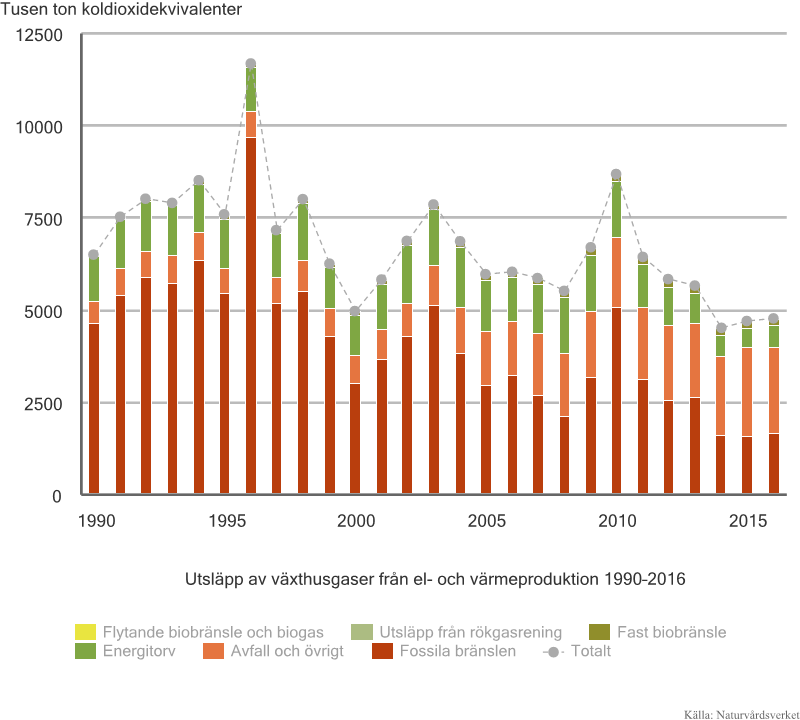
\includegraphics[scale=0.7]{naturvard-co2}
	\caption{Statistik ifrån naturvårdsverket}
	\label{natuvard-co2}
\end{figure*}


\subsection{Miljöpåverkan av utvecklingsprocessen}
Enligt \ref{natuvard-co2} så skapade Sveriges el och värmeproduktion ett CO2 utsläpp på $4781*10^6$ gram år 2016. Kombinerat med att Sveriges energi produktion detta år var 152 TWh enligt Energimyndighetens pressmeddelande\cite{elprod2016}, så får vi att varje kWh i genomsnitt skapade ett utsläpp på: $4781*10^9 / (152 * 10^{12}) \approx 31.45 * 10^{-3}$ gram CO2 per kWh. Ifrån tidigare approximerades gruppens kWh till $17.28 + 491.52 = 508.8$ vilket ger oss ett CO2 utsläpp på: $$31.45 * 10^{-3} * 508.8 \approx 16 \text{ gram CO2}$$


\section{Diskussion}
\label{sec:joel_a-discussion}

\subsection{Utvecklingsprocessens miljöpåverkan}
Gruppens approximerade utsläpp på 24.8 gram C02 är grov approximering och missar utsläpp ifrån flera faktorer såsom strömmen kaffemaskinen använde och strömmen molntjänsterna använde. Så uppskattningen är sannolikt en underdrift, men trots det så är ett koldioxid utsläpp under 25 gram högst marginelt med tanke på omfattningen av utvecklingsprocessen. De mest sannolika faktorerna för det låga värmen är antagligen det låga CO2 utsläppet av energi producerat ifrån vatten och kärnkraft som representerar runt 90\% av sveriges eltillverkning (TODO källa). Den andra viktiga faktorn är hur småskalig utvecklingen av produkten var, med enbart åtta personer och utan stor utrustning såsom serverhallar så används helt enkelt inte en mängd elektricitet som är relevant ur ett storskaligt miljöperspektiv. Nivå ett effekterna verkar alltså inte ha haft någon större påverkan på hållbar utveckling.


\subsection{Produktens miljöpåverkan}
Produkten har ännu inte använts vid skrivandet av denna rapport så den har inte haft någon miljöpåverkan förutom dess utvecklingsprocess som beskrevs ovan. Men de nivå två effekterna som den kan tänka sig ha, såsom att den uppmuntrar fler företag att skapa ett spel för sina presentationer på mässor, verkar inte vara något att oroa sig över då den låga påverkan gruppens utvecklingsprocess haft på miljön. Dock är det värt att notera att ifall en sådan mjukvara utvecklas på en plats där elektriciteten framställs på ett mer omiljövänligt sätt så kan denna process vara påtagligt värre för miljön. Detta är dock väldigt spekulativt och det är osannolikt att ett studentarbete i praktiken skulle skapa stora vågeffekter i hur mjukvara utvecklas. Troligtvis så kommer inga nivå två eller tre effekter att skapas utifrån produkten gruppen sammanställt.

\section{Slutsatser}
\label{sec:joel_a-conclusion}

*Vad kunde gjorts annorlunda vid utvecklingen?


*Var det ett rimligt beslut att ignorera miljöfaktorn i utvecklingen?


\chapter{Lieths del}

\section{Introduktion}
\label{sec:Lieth-introduction}

Kommunikation och information expanderar snabbare än någonsin idag. Som ett resultat, detta lägger stor press på dagens mjukvaruutveckling. 
Detta innebär att för ett mjukvaruutvecklingsprojekt att nå sina uppsatta mål måste utvecklingsprocessen optimeras så långt som möjligt [8]. 
En av dem mest tillämpade arbetsmetodik för sådan optimering är agil systemutvecklingsmetodiken. Agil systemutveckling är av de mest populära 
arbetsmetodiker bland små lika väl som stora mjukvaruprojekt. Agil systemutveckling har sett en stor intresseökning under dem senast åren [6]. 
På dess enklaste form agility definieras som förmågan att skapa och anpassa sig till förändring för att uppnå en slutprodukt, tjänst eller mål av 
ett projekt . Denna rapport kommer handla om tillämpning av en specifik form agil mjukvaruutvecklingsmetodik, nämligen Scrum. 
\\
\\ Scrum är agil mjukvaruutveckling ramverk som syftar till att hjälpa utvecklingsteamen att effektiviseras. Scrum är en av de mest tillämpade agil 
arbetsmetodiker. Den förser ett smidigt arbetssätt som syftar till att förbättra produktivitet i ett utvecklingsprojekt och effektivisera utvecklingsprocessen [7].

\subsection{Syfte \& Mål}
\label{subsec:Lieth-aim}
Syftet med denna rapporten är att utforska hur kan agil arbetsmetodik såsom Scrum bidra till att effektivisera teamsamarbete och eventuellt hjälpa teamet att 
uppnå de uppsatta målen och vad kan användas för göra framsteg i processen.


subsection{Frågeställning}
\label{subsec:Lieth-research-questions}
För att göra denna undersökninen krävs några fundementala frågor som behöver besvaras, dessa presenteras nedan:

\begin{enumerate}
	\item Vilka delar av Scrum bör vara med i vår Scrum version som kan bidra till att effektivisera vårt teamsamarbete 
	och eventuellt skapa bättre värde för vår kund?
	\item Hur börScrum planeras på sådant sätt att det skapar värde för kunden samtidigt som kursens lärandemålen uppnås? 
	
	
	\item Finns det fler verktyg, t.ex. Trello eller Github som kan användas till att göra vår  Scrum-version bättre på att skapa värde till kunden? 
	
\end{enumerate}

\subsection{Avgränsingar}
\label{subsec:Lieth-delimitations}
Resultaten som presenteras i detta papper är baserat på som läser programmen civilingenjör i datateknik samt civilingenjör i mjukvarateknik och förutser att
ingen av gruppmedlemmerna har tidigare haft något kurs eller erfarenhet inom agil mjukvaruutveckling. Dessutom, var studien begränsad av tidsbudget på 
400 timmar per person där fler obligatirska kursmoment var en del av.



\section{Bakgrund}
\label{sec:Lieth-background}
Många företag idag använder, håller på att bygga, eller planerar att bygga någon form av molntjänst. Detta innebär att antalet fysiska objekt som är eller 
kommer bli uppkopplade till internet, för att jobba mot ett gemensamt mål, ökar. Cybercom Sweden är ett IT-konsultbolag som hjälper andra företag att 
digitaliseras samt erbjuder tekniska lösningar. När vi, grupp ett, blev utvalda att utföra vårt kandidatprojekt hos Cybercom Sweden, visste vi vad som 
behöver göras. Men det som vi var osäkra på är hur vi skulle dela arbetet sådant att  alla medlemmar i teamet kan jobba på ett produktivt och effektivt 
sätt. Därför bestämde vi att jobb agilt. Redan under första dagarna i bestämde vi som grupp att använda Scrum som agil arbetsmetodik och Trello som 
hjälpverktyg för att hålla koll på vad vi har att utför, vad som utförs just nu, och vad som har utförts. Som utvecklingsledare jag tog på mig att undersöka 
sätten som hjälper oss som grupp att uppnå vår uppsatta mål. 

\section{Teori}
\label{sec:Lieth-Teori}
Agila metoder, såsom Scrum, har sett en märkbar tillväxt i popularitet inom mjukvaruutveckling kontext som karakteriseras av höga ostadighet[6]. I ett Scrum 
tillvägagångssätt team deltagare jobbar ihop för att föra projektet framåt genom att använda s.k Scrum verktyg som t.ex Scrum board, Scrum möte, burndown 
charts[7]. Detta möjliggöra för teamet att vara medvetna om senaste ändringar i kraven och om-prioriterar om det sådant behövs[7]. 

Eftersom Scrum metodiken är väldigt flexibel och kan ändras sådant att den passar varje grupps behov vi bestämde oss att har endast följande delar av scrum:

\begin{enumerate}
	\item Sprintplanering

	\item Scrum board  i form av Trello board
	
	\item Scrum möten i form av veckomöte online kommunikation via Slack
	
	\item Veckorapporter och burndown charts
	
\end{enumerate}

\section{Metod}
\label{sec:Lieth-Metod}
Detta avsnitt går i detaljer om hur vår Scrum version är uppbyggd och vad som förväntas av varje del.

\subsection{Sprintplannering}
\label{subsec:Lieth-Sprintplannering}
Varje sprint är 2 veckor lång. under varje sprint så jobbade teamet mot en del problem. Detta gjorde det lättare 
för teamet att jobba effektivare, då stora problem är delade i små delproblem som gör det lättare att tackla problemen 
samt att berätta vad  har gjort vid veckomöten. Vid slutet av varje sprint gruppen höll ett möte för att skapa en 
statusrapport på vad som har utförts under sprinten och ifall den sprintents uppsatta målen är mötta eller inte.


\subsection{Scrum Board}
\label{subsec:Lieth-Scrum Board}
Scrum board är gjordes i form av Trello aktiviteter. Detta möjliggjorde spårning av målen samt underlättade för gruppen att ha 
koll på vad som finns kvar att utföra, vad som utförs, och vad som har utförts. inför start av varje sprint, teamet höll ett möte 
för att planera vad som behöver göras under kommande sprint, vilka skulle göra vad, och hur lång tid varje aktivitet skulle ta. 
Aktiviteterna skrevs i form Trello aktiviteter och las enligt dess status, dvs att utföra, under utförande, utfördes osv.

\subsection{Scrum Möten}
\label{subsec:Lieth-Scrum Möten}
Inför varje av varje sprint hölls ett Scrum möte. under de möten diskuterades vad som skulle utföras, hur det skulle utföras och 
vad vi har lärt oss från tidigare sprinten. De möten var väldigt viktiga för att veta exakt vart teamet befann oss i vår plan av att 
skapa ett värde för kunden. Dessutom, diskuterade teamet risker och hur de borde hanteras.  
\\
\\Vid slutet av varje sprint hölls ett annat möte. Under detta diskuterade teamet vad som har gått bra, vad som måste förbättras 
och hur skulle vi kunna använda vår erfarenheter från tidigare sprint för att skapa bättre värde för kunden i varande sprinten. 

\subsection{Veckorapporter}
\label{subsec:Lieth-Veckorapporter}
Vid början av varje vecka ett veckomöte hölls. Veckorapporter bestod av tidrapportering som gjordes löpande under projektets 
gång, burndown charts, och statusuppdatering om olika projekt relaterade aktiviteter. Under de möten diskuterade teammedlemmar 
vad har gjorts under förra veckan, vad ska göras nästa vecka och vilka risker finns det. En veckorapport skrevs vid mötestillfällen. 
Burndown charts gjorde det lättare att veta hur mycket jobb har lagts på vad samt hur många timmar har varje medlem i teamet 
kvar att göra. 

\input{individuall/Lieth/Lieth-Resultat}
\input{individuall/Lieth/Lieth-Diskussion}
\input{individuall/Lieth/Lieth-Slutsats}



\printbibliography

\end{document}

%%%%%%%%%%%%%%%%%%%%%%%%%%%%%%%%%%%%%%%%%%%%%%%%%%%%%%%%%%%%%%%%%%%%%%
%%% demothesis.tex ends here
